

%% bare_jrnl_compsoc.tex
%% V1.4a
%% 2014/09/17
%% by Michael Shell
%% See:
%% http://www.michaelshell.org/
%% for current contact information.
%%
%% This is a skeleton file demonstrating the use of IEEEtran.cls
%% (requires IEEEtran.cls version 1.8a or later) with an IEEE
%% Computer Society journal paper.
%%
%% Support sites:
%% http://www.michaelshell.org/tex/ieeetran/
%% http://www.ctan.org/tex-archive/macros/latex/contrib/IEEEtran/
%% and
%% http://www.ieee.org/

%%*************************************************************************
%% Legal Notice:
%% This code is offered as-is without any warranty either expressed or
%% implied; without even the implied warranty of MERCHANTABILITY or
%% FITNESS FOR A PARTICULAR PURPOSE! 
%% User assumes all risk.
%% In no event shall IEEE or any contributor to this code be liable for
%% any damages or losses, including, but not limited to, incidental,
%% consequential, or any other damages, resulting from the use or misuse
%% of any information contained here.
%%
%% All comments are the opinions of their respective authors and are not
%% necessarily endorsed by the IEEE.
%%
%% This work is distributed under the LaTeX Project Public License (LPPL)
%% ( http://www.latex-project.org/ ) version 1.3, and may be freely used,
%% distributed and modified. A copy of the LPPL, version 1.3, is included
%% in the base LaTeX documentation of all distributions of LaTeX released
%% 2003/12/01 or later.
%% Retain all contribution notices and credits.
%% ** Modified files should be clearly indicated as such, including  **
%% ** renaming them and changing author support contact information. **
%%
%% File list of work: IEEEtran.cls, IEEEtran_HOWTO.pdf, bare_adv.tex,
%%                    bare_conf.tex, bare_jrnl.tex, bare_conf_compsoc.tex,
%%                    bare_jrnl_compsoc.tex, bare_jrnl_transmag.tex
%%*************************************************************************


% *** Authors should verify (and, if needed, correct) their LaTeX system  ***
% *** with the testflow diagnostic prior to trusting their LaTeX platform ***
% *** with production work. IEEE's font choices and paper sizes can       ***
% *** trigger bugs that do not appear when using other class files.       ***                          ***
% The testflow support page is at:
% http://www.michaelshell.org/tex/testflow/


\documentclass[10pt,journal,compsoc]{IEEEtran}
%
% If IEEEtran.cls has not been installed into the LaTeX system files,
% manually specify the path to it like:
% \documentclass[10pt,journal,compsoc]{../sty/IEEEtran}



\usepackage{calc}


\usepackage{url}
%\usepackage{algorithm, algorithmic}
\usepackage{amsmath}
\usepackage{epsfig}
\usepackage{graphicx}
\usepackage{subfig}

%\graphicspath{{eps/}}
\usepackage{amsbsy}
\usepackage{amssymb}
\usepackage{verbatim}
\usepackage{multirow}
%\usepackage{cite}

\usepackage[linesnumbered,ruled,vlined]{algorithm2e}
\usepackage{enumitem}
\usepackage{balance}
\usepackage{lscape}
\usepackage{float}
\usepackage{longtable}
\usepackage{array}
\usepackage{framed}
\usepackage{epstopdf}
%\usepackage{times}
\usepackage{comment}
\usepackage{pifont}
\usepackage{color}

\usepackage[labelfont=bf]{caption}
% Adjust whitespace above and below captions
\addtolength{\abovecaptionskip}{-4pt}
\addtolength{\belowcaptionskip}{-8pt}

% Some very useful LaTeX packages include:
% (uncomment the ones you want to load)


% *** MISC UTILITY PACKAGES ***
%
%\usepackage{ifpdf}
% Heiko Oberdiek's ifpdf.sty is very useful if you need conditional
% compilation based on whether the output is pdf or dvi.
% usage:
% \ifpdf
%   % pdf code
% \else
%   % dvi code
% \fi
% The latest version of ifpdf.sty can be obtained from:
% http://www.ctan.org/tex-archive/macros/latex/contrib/oberdiek/
% Also, note that IEEEtran.cls V1.7 and later provides a builtin
% \ifCLASSINFOpdf conditional that works the same way.
% When switching from latex to pdflatex and vice-versa, the compiler may
% have to be run twice to clear warning/error messages.






% *** CITATION PACKAGES ***
%
\ifCLASSOPTIONcompsoc
  % IEEE Computer Society needs nocompress option
  % requires cite.sty v4.0 or later (November 2003)
  \usepackage[nocompress]{cite}
\else
  % normal IEEE
  \usepackage{cite}
\fi
% cite.sty was written by Donald Arseneau
% V1.6 and later of IEEEtran pre-defines the format of the cite.sty package
% \cite{} output to follow that of IEEE. Loading the cite package will
% result in citation numbers being automatically sorted and properly
% "compressed/ranged". e.g., [1], [9], [2], [7], [5], [6] without using
% cite.sty will become [1], [2], [5]--[7], [9] using cite.sty. cite.sty's
% \cite will automatically add leading space, if needed. Use cite.sty's
% noadjust option (cite.sty V3.8 and later) if you want to turn this off
% such as if a citation ever needs to be enclosed in parenthesis.
% cite.sty is already installed on most LaTeX systems. Be sure and use
% version 5.0 (2009-03-20) and later if using hyperref.sty.
% The latest version can be obtained at:
% http://www.ctan.org/tex-archive/macros/latex/contrib/cite/
% The documentation is contained in the cite.sty file itself.
%
% Note that some packages require special options to format as the Computer
% Society requires. In particular, Computer Society  papers do not use
% compressed citation ranges as is done in typical IEEE papers
% (e.g., [1]-[4]). Instead, they list every citation separately in order
% (e.g., [1], [2], [3], [4]). To get the latter we need to load the cite
% package with the nocompress option which is supported by cite.sty v4.0
% and later. Note also the use of a CLASSOPTION conditional provided by
% IEEEtran.cls V1.7 and later.





% *** GRAPHICS RELATED PACKAGES ***
%
\ifCLASSINFOpdf
  % \usepackage[pdftex]{graphicx}
  % declare the path(s) where your graphic files are
  % \graphicspath{{../pdf/}{../jpeg/}}
  % and their extensions so you won't have to specify these with
  % every instance of \includegraphics
  % \DeclareGraphicsExtensions{.pdf,.jpeg,.png}
\else
  % or other class option (dvipsone, dvipdf, if not using dvips). graphicx
  % will default to the driver specified in the system graphics.cfg if no
  % driver is specified.
  % \usepackage[dvips]{graphicx}
  % declare the path(s) where your graphic files are
  % \graphicspath{{../eps/}}
  % and their extensions so you won't have to specify these with
  % every instance of \includegraphics
  % \DeclareGraphicsExtensions{.eps}
\fi
% graphicx was written by David Carlisle and Sebastian Rahtz. It is
% required if you want graphics, photos, etc. graphicx.sty is already
% installed on most LaTeX systems. The latest version and documentation
% can be obtained at: 
% http://www.ctan.org/tex-archive/macros/latex/required/graphics/
% Another good source of documentation is "Using Imported Graphics in
% LaTeX2e" by Keith Reckdahl which can be found at:
% http://www.ctan.org/tex-archive/info/epslatex/
%
% latex, and pdflatex in dvi mode, support graphics in encapsulated
% postscript (.eps) format. pdflatex in pdf mode supports graphics
% in .pdf, .jpeg, .png and .mps (metapost) formats. Users should ensure
% that all non-photo figures use a vector format (.eps, .pdf, .mps) and
% not a bitmapped formats (.jpeg, .png). IEEE frowns on bitmapped formats
% which can result in "jaggedy"/blurry rendering of lines and letters as
% well as large increases in file sizes.
%
% You can find documentation about the pdfTeX application at:
% http://www.tug.org/applications/pdftex






% *** MATH PACKAGES ***
%
%\usepackage[cmex10]{amsmath}
% A popular package from the American Mathematical Society that provides
% many useful and powerful commands for dealing with mathematics. If using
% it, be sure to load this package with the cmex10 option to ensure that
% only type 1 fonts will utilized at all point sizes. Without this option,
% it is possible that some math symbols, particularly those within
% footnotes, will be rendered in bitmap form which will result in a
% document that can not be IEEE Xplore compliant!
%
% Also, note that the amsmath package sets \interdisplaylinepenalty to 10000
% thus preventing page breaks from occurring within multiline equations. Use:
%\interdisplaylinepenalty=2500
% after loading amsmath to restore such page breaks as IEEEtran.cls normally
% does. amsmath.sty is already installed on most LaTeX systems. The latest
% version and documentation can be obtained at:
% http://www.ctan.org/tex-archive/macros/latex/required/amslatex/math/





% *** SPECIALIZED LIST PACKAGES ***
%
%\usepackage{algorithmic}
% algorithmic.sty was written by Peter Williams and Rogerio Brito.
% This package provides an algorithmic environment fo describing algorithms.
% You can use the algorithmic environment in-text or within a figure
% environment to provide for a floating algorithm. Do NOT use the algorithm
% floating environment provided by algorithm.sty (by the same authors) or
% algorithm2e.sty (by Christophe Fiorio) as IEEE does not use dedicated
% algorithm float types and packages that provide these will not provide
% correct IEEE style captions. The latest version and documentation of
% algorithmic.sty can be obtained at:
% http://www.ctan.org/tex-archive/macros/latex/contrib/algorithms/
% There is also a support site at:
% http://algorithms.berlios.de/index.html
% Also of interest may be the (relatively newer and more customizable)
% algorithmicx.sty package by Szasz Janos:
% http://www.ctan.org/tex-archive/macros/latex/contrib/algorithmicx/




% *** ALIGNMENT PACKAGES ***
%
%\usepackage{array}
% Frank Mittelbach's and David Carlisle's array.sty patches and improves
% the standard LaTeX2e array and tabular environments to provide better
% appearance and additional user controls. As the default LaTeX2e table
% generation code is lacking to the point of almost being broken with
% respect to the quality of the end results, all users are strongly
% advised to use an enhanced (at the very least that provided by array.sty)
% set of table tools. array.sty is already installed on most systems. The
% latest version and documentation can be obtained at:
% http://www.ctan.org/tex-archive/macros/latex/required/tools/


% IEEEtran contains the IEEEeqnarray family of commands that can be used to
% generate multiline equations as well as matrices, tables, etc., of high
% quality.




% *** SUBFIGURE PACKAGES ***
%\ifCLASSOPTIONcompsoc
%  \usepackage[caption=false,font=footnotesize,labelfont=sf,textfont=sf]{subfig}
%\else
%  \usepackage[caption=false,font=footnotesize]{subfig}
%\fi
% subfig.sty, written by Steven Douglas Cochran, is the modern replacement
% for subfigure.sty, the latter of which is no longer maintained and is
% incompatible with some LaTeX packages including fixltx2e. However,
% subfig.sty requires and automatically loads Axel Sommerfeldt's caption.sty
% which will override IEEEtran.cls' handling of captions and this will result
% in non-IEEE style figure/table captions. To prevent this problem, be sure
% and invoke subfig.sty's "caption=false" package option (available since
% subfig.sty version 1.3, 2005/06/28) as this is will preserve IEEEtran.cls
% handling of captions.
% Note that the Computer Society format requires a sans serif font rather
% than the serif font used in traditional IEEE formatting and thus the need
% to invoke different subfig.sty package options depending on whether
% compsoc mode has been enabled.
%
% The latest version and documentation of subfig.sty can be obtained at:
% http://www.ctan.org/tex-archive/macros/latex/contrib/subfig/




% *** FLOAT PACKAGES ***
%
%\usepackage{fixltx2e}
% fixltx2e, the successor to the earlier fix2col.sty, was written by
% Frank Mittelbach and David Carlisle. This package corrects a few problems
% in the LaTeX2e kernel, the most notable of which is that in current
% LaTeX2e releases, the ordering of single and double column floats is not
% guaranteed to be preserved. Thus, an unpatched LaTeX2e can allow a
% single column figure to be placed prior to an earlier double column
% figure. The latest version and documentation can be found at:
% http://www.ctan.org/tex-archive/macros/latex/base/


%\usepackage{stfloats}
% stfloats.sty was written by Sigitas Tolusis. This package gives LaTeX2e
% the ability to do double column floats at the bottom of the page as well
% as the top. (e.g., "\begin{figure*}[!b]" is not normally possible in
% LaTeX2e). It also provides a command:
%\fnbelowfloat
% to enable the placement of footnotes below bottom floats (the standard
% LaTeX2e kernel puts them above bottom floats). This is an invasive package
% which rewrites many portions of the LaTeX2e float routines. It may not work
% with other packages that modify the LaTeX2e float routines. The latest
% version and documentation can be obtained at:
% http://www.ctan.org/tex-archive/macros/latex/contrib/sttools/
% Do not use the stfloats baselinefloat ability as IEEE does not allow
% \baselineskip to stretch. Authors submitting work to the IEEE should note
% that IEEE rarely uses double column equations and that authors should try
% to avoid such use. Do not be tempted to use the cuted.sty or midfloat.sty
% packages (also by Sigitas Tolusis) as IEEE does not format its papers in
% such ways.
% Do not attempt to use stfloats with fixltx2e as they are incompatible.
% Instead, use Morten Hogholm'a dblfloatfix which combines the features
% of both fixltx2e and stfloats:
%
% \usepackage{dblfloatfix}
% The latest version can be found at:
% http://www.ctan.org/tex-archive/macros/latex/contrib/dblfloatfix/




%\ifCLASSOPTIONcaptionsoff
%  \usepackage[nomarkers]{endfloat}
% \let\MYoriglatexcaption\caption
% \renewcommand{\caption}[2][\relax]{\MYoriglatexcaption[#2]{#2}}
%\fi
% endfloat.sty was written by James Darrell McCauley, Jeff Goldberg and 
% Axel Sommerfeldt. This package may be useful when used in conjunction with 
% IEEEtran.cls'  captionsoff option. Some IEEE journals/societies require that
% submissions have lists of figures/tables at the end of the paper and that
% figures/tables without any captions are placed on a page by themselves at
% the end of the document. If needed, the draftcls IEEEtran class option or
% \CLASSINPUTbaselinestretch interface can be used to increase the line
% spacing as well. Be sure and use the nomarkers option of endfloat to
% prevent endfloat from "marking" where the figures would have been placed
% in the text. The two hack lines of code above are a slight modification of
% that suggested by in the endfloat docs (section 8.4.1) to ensure that
% the full captions always appear in the list of figures/tables - even if
% the user used the short optional argument of \caption[]{}.
% IEEE papers do not typically make use of \caption[]'s optional argument,
% so this should not be an issue. A similar trick can be used to disable
% captions of packages such as subfig.sty that lack options to turn off
% the subcaptions:
% For subfig.sty:
% \let\MYorigsubfloat\subfloat
% \renewcommand{\subfloat}[2][\relax]{\MYorigsubfloat[]{#2}}
% However, the above trick will not work if both optional arguments of
% the \subfloat command are used. Furthermore, there needs to be a
% description of each subfigure *somewhere* and endfloat does not add
% subfigure captions to its list of figures. Thus, the best approach is to
% avoid the use of subfigure captions (many IEEE journals avoid them anyway)
% and instead reference/explain all the subfigures within the main caption.
% The latest version of endfloat.sty and its documentation can obtained at:
% http://www.ctan.org/tex-archive/macros/latex/contrib/endfloat/
%
% The IEEEtran \ifCLASSOPTIONcaptionsoff conditional can also be used
% later in the document, say, to conditionally put the References on a 
% page by themselves.




% *** PDF, URL AND HYPERLINK PACKAGES ***
%
%\usepackage{url}
% url.sty was written by Donald Arseneau. It provides better support for
% handling and breaking URLs. url.sty is already installed on most LaTeX
% systems. The latest version and documentation can be obtained at:
% http://www.ctan.org/tex-archive/macros/latex/contrib/url/
% Basically, \url{my_url_here}.





% *** Do not adjust lengths that control margins, column widths, etc. ***
% *** Do not use packages that alter fonts (such as pslatex).         ***
% There should be no need to do such things with IEEEtran.cls V1.6 and later.
% (Unless specifically asked to do so by the journal or conference you plan
% to submit to, of course. )


% correct bad hyphenation here
\hyphenation{op-tical net-works semi-conduc-tor}


\begin{document}
%
% paper title
% Titles are generally capitalized except for words such as a, an, and, as,
% at, but, by, for, in, nor, of, on, or, the, to and up, which are usually
% not capitalized unless they are the first or last word of the title.
% Linebreaks \\ can be used within to get better formatting as desired.
% Do not put math or special symbols in the title.
%\title{Bare Demo of IEEEtran.cls\\ for Computer Society Journals}
\title{In-Storage Computing for Hadoop MapReduce Framework}
%
%
% author names and IEEE memberships
% note positions of commas and nonbreaking spaces ( ~ ) LaTeX will not break
% a structure at a ~ so this keeps an author's name from being broken across
% two lines.
% use \thanks{} to gain access to the first footnote area
% a separate \thanks must be used for each paragraph as LaTeX2e's \thanks
% was not built to handle multiple paragraphs
%
%
%\IEEEcompsocitemizethanks is a special \thanks that produces the bulleted
% lists the Computer Society journals use for "first footnote" author
% affiliations. Use \IEEEcompsocthanksitem which works much like \item
% for each affiliation group. When not in compsoc mode,
% \IEEEcompsocitemizethanks becomes like \thanks and
% \IEEEcompsocthanksitem becomes a line break with idention. This
% facilitates dual compilation, although admittedly the differences in the
% desired content of \author between the different types of papers makes a
% one-size-fits-all approach a daunting prospect. For instance, compsoc 
% journal papers have the author affiliations above the "Manuscript
% received ..."  text while in non-compsoc journals this is reversed. Sigh.

%\author{Michael~Shell,~\IEEEmembership{Member,~IEEE,}
%        John~Doe,~\IEEEmembership{Fellow,~OSA,}
%        and~Jane~Doe,~\IEEEmembership{Life~Fellow,~IEEE}% <-this % stops a space
				
				
\author{Dongchul~Park,~\IEEEmembership{Member,~IEEE,}
        Kwanghyun~Park,~\IEEEmembership{Member,~IEEE,}
        Yang-Suk~Kee,~\IEEEmembership{Member,~IEEE,}				
        and~Jignesh~M.~Patel,~\IEEEmembership{Fellow,~IEEE}% <-this % stops a space				
				
				
				
%\IEEEcompsocitemizethanks{\IEEEcompsocthanksitem M. Shell is with the Department
%of Electrical and Computer Engineering, Georgia Institute of Technology, Atlanta,
%GA, 30332.\protect\\
% note need leading \protect in front of \\ to get a newline within \thanks as
% \\ is fragile and will error, could use \hfil\break instead.
%E-mail: see http://www.michaelshell.org/contact.html
%\IEEEcompsocthanksitem J. Doe and J. Doe are with Anonymous University.}% <-this % stops an unwanted space
%\thanks{Manuscript received April 19, 2005; revised September 17, 2014.}}



\IEEEcompsocitemizethanks{\IEEEcompsocthanksitem Dongchul Park and Yang-Suk Kee are with the System Architecture Lab. (SAL) of Samsung Semiconductor Inc., San Jose, CA 95134. E-mail: \{dongchul.p1, yangseok.ki\}@ssi.samsung.com\protect\\
% note need leading \protect in front of \\ to get a newline within \thanks as
% \\ is fragile and will error, could use \hfil\break instead.

\IEEEcompsocthanksitem Kwanghyun Park and Jignesh M. Patel are with the Department of Computer Science, University of Wisconsin--Madison, Madision, WI 85123. E-mail: kpark, j.patel@cs.wisc.edu}% <-this % stops a space
\thanks{Manuscript received April 19, 2005; revised September 17, 2014.}}








% note the % following the last \IEEEmembership and also \thanks - 
% these prevent an unwanted space from occurring between the last author name
% and the end of the author line. i.e., if you had this:
% 
% \author{....lastname \thanks{...} \thanks{...} }
%                     ^------------^------------^----Do not want these spaces!
%
% a space would be appended to the last name and could cause every name on that
% line to be shifted left slightly. This is one of those "LaTeX things". For
% instance, "\textbf{A} \textbf{B}" will typeset as "A B" not "AB". To get
% "AB" then you have to do: "\textbf{A}\textbf{B}"
% \thanks is no different in this regard, so shield the last } of each \thanks
% that ends a line with a % and do not let a space in before the next \thanks.
% Spaces after \IEEEmembership other than the last one are OK (and needed) as
% you are supposed to have spaces between the names. For what it is worth,
% this is a minor point as most people would not even notice if the said evil
% space somehow managed to creep in.



% The paper headers
%\markboth{Journal of \LaTeX\ Class Files,~Vol.~13, No.~9, September~2014}%
%{Shell \MakeLowercase{\textit{et al.}}: Bare Demo of IEEEtran.cls for Computer Society Journals}


\markboth{IEEE Transactions on Computers, February~2015}%
{Park \MakeLowercase{\textit{et al.}}: In-Storage Computing for Hadoop MapReduce Framework}


% The only time the second header will appear is for the odd numbered pages
% after the title page when using the twoside option.
% 
% *** Note that you probably will NOT want to include the author's ***
% *** name in the headers of peer review papers.                   ***
% You can use \ifCLASSOPTIONpeerreview for conditional compilation here if
% you desire.



% The publisher's ID mark at the bottom of the page is less important with
% Computer Society journal papers as those publications place the marks
% outside of the main text columns and, therefore, unlike regular IEEE
% journals, the available text space is not reduced by their presence.
% If you want to put a publisher's ID mark on the page you can do it like
% this:
%\IEEEpubid{0000--0000/00\$00.00~\copyright~2014 IEEE}
% or like this to get the Computer Society new two part style.
%\IEEEpubid{\makebox[\columnwidth]{\hfill 0000--0000/00/\$00.00~\copyright~2014 IEEE}%
%\hspace{\columnsep}\makebox[\columnwidth]{Published by the IEEE Computer Society\hfill}}
% Remember, if you use this you must call \IEEEpubidadjcol in the second
% column for its text to clear the IEEEpubid mark (Computer Society jorunal
% papers don't need this extra clearance.)



% use for special paper notices
%\IEEEspecialpapernotice{(Invited Paper)}



% for Computer Society papers, we must declare the abstract and index terms
% PRIOR to the title within the \IEEEtitleabstractindextext IEEEtran
% command as these need to go into the title area created by \maketitle.
% As a general rule, do not put math, special symbols or citations
% in the abstract or keywords.
\IEEEtitleabstractindextext{%
\begin{abstract}
Solid State Drives (SSDs) have been developed for the replacement of conventional magnetic Hard Disk Drives (HDDs) as a faster storage device. Their high computational capabilities, however, enable SSDs to become a computing node, not just another faster storage device, which is called In-Storage Computing (ISC). Hadoop MapReduce framework nowadays became a de facto standard for big data processing. 
This paper explores the challenges and opportunities of In-Storage Computing for Hadoop MapReduce framework. 
For this, we co-design a Hadoop MapReduce system and an ISC device by implementing the Mapper inside real SSD firmware and offloading Map tasks from a host MapReduce system to the SSDs. Then, we make extensive experiments in real Hadoop clusters. 
Our experiment results demonstrate that our ISC Hadoop MapReduce system achieves a remarkable performance gain (2$\times$ faster) as well as significant energy saving (9.3$\times$ lower). 
\end{abstract}

% Note that keywords are not normally used for peerreview papers.
\begin{IEEEkeywords}
In-Storage Computing, Storage Intelligence, In-Situ Processing, Near data processing, Smart SSD, Hadoop, MapReduce, Big Data.
\end{IEEEkeywords}}


% make the title area
\maketitle


% To allow for easy dual compilation without having to reenter the
% abstract/keywords data, the \IEEEtitleabstractindextext text will
% not be used in maketitle, but will appear (i.e., to be "transported")
% here as \IEEEdisplaynontitleabstractindextext when the compsoc 
% or transmag modes are not selected <OR> if conference mode is selected 
% - because all conference papers position the abstract like regular
% papers do.
\IEEEdisplaynontitleabstractindextext
% \IEEEdisplaynontitleabstractindextext has no effect when using
% compsoc or transmag under a non-conference mode.



% For peer review papers, you can put extra information on the cover
% page as needed:
% \ifCLASSOPTIONpeerreview
% \begin{center} \bfseries EDICS Category: 3-BBND \end{center}
% \fi
%
% For peerreview papers, this IEEEtran command inserts a page break and
% creates the second title. It will be ignored for other modes.
\IEEEpeerreviewmaketitle







\section{Introduction}\label{sec:introduction}

\IEEEPARstart{D}{ue} to the superior characteristics of Solid State Drives (SSDs) to the rotational Hard Disk Drives (HDDs), SSDs have been increasingly adopted even in enterprise systems as well as in personal/mobile systems~\cite{BPLRU:FAST:2008,CFTL:SIGMETRICS:2010,GORDON:ASPLOS:2009}. Originally, SSDs have been developed for the purpose of replacing the traditional HDDs as a faster storage device since, for instance, modern SSDs are over 100 times faster than HDDs in accessing data. Moreover, they consume over 10 times less energy than HDDs~\cite{Samsung:WhitePaper:2014}. Thus, most of the recent research studies have focused primarily on how to make use of SSDs as yet-another-faster HDDs.


However, high computational capabilities of the modern SSDs had people start to rethink of SSDs as, not just a faster storage device, but another type of a computing node, so-called In-Storage Computing (for short, ISC). Unlike a traditional CPU-centric computing philosophy--''moving data closer to codes'', this ISC model suggests a totally different computing paradigm--''moving codes closer to data'' thereby offloading key functions from a host system to a device, which significantly changes a data flow for computation~\cite{NearDataProcessing:Micro:2014}. This data flow change enables the ISC system to achieve not only a faster performance but also a marvelous energy saving, which results in the notable savings of Total Cost of Ownership (TCO) in the long run. This ISC computing paradigm is newly spotlighted in the big data era these days.


Hadoop MapReduce is a software framework for the distributed processing of large data sets on clusters of commodity hardware, and MapReduce framework nowadays became a de facto standard for big data processing~\cite{MapReduce:Tutorial}. In the MapReduce framework, computation is divided into two functions: Map and Reduce. Mapper takes a set of data and converts it into another set of data (i.e., intermediate data), where individual elements are composed of key/value pairs. The Reducer takes the outputs from Mappers as input and combines those intermediate data into a smaller set of key/value tuples~\cite{MapReduce:OSDI:2004}.
The Hadoop MapReduce system tries to collocate the data in a local computing node to take advantage of data locality, which is at the heart of MapReduce and is the reason for its good performance~\cite{TomWhite:HadoopDefinitiveGuide:2012}. This Hadoop policy--''putting computation near the data'' aligns well with the aforementioned recent computing paradigm shift, which was also early advocated by Jim Gray~\cite{JimGray:MSRTR:2003}.


This work explores the challenges and opportunities of In-Storage Computing for the Hadoop MapReduce framework. We offload Mapper into the ISC device (i.e., SSD) by implementing Map features inside real SSD firmware and integrate our ISC Hadoop framework into the existing Hadoop MapReduce system framework. We set up Hadoop clusters and run a Hadoop MapReduce application on the clusters to verify our holistic ISC Hadoop framework. Our experiment results show that the ISC Hadoop system achieves a remarkable performance gain (2$\times$ faster) and significantly reduces energy consumption (more than 9$\times$ lower). 

The system co-design of our ISC Hadoop MapReduce causes several interesting and very challenging issues as follows.

\textbf{Discrepancy in data representation}: For data access, Hadoop in the host uses file systems such as Hadoop Distributed File System (HDFS) and a local file system such as EXT3/4. However, an ISC device cannot rely on any file system information and, instead, uses different data representation such as a Logical Block Address (LBA). Therefore, a host Hadoop system should be able to collaborate with ISC devices by employing LBA information, not using any file systems.
%To address this issue, we develop a software component that is in charge of converting a file name into LBA range information lists.

%\textbf{Discrepancy in Data Representation}: For data access, Hadoop in the host uses file systems such as Hadoop Distributed File System (HDFS) and a local file system such as EXT3/4. However, an ISC device cannot rely on any file system information and, instead, uses different data representation such as Logical Block Address (LBA). To address this issue, we develop a software component that is in charge of converting a file name into LBA range information lists.


\textbf{Discrepancy in system interfaces}: System interfaces between the Hadoop framework in the host system and an ISC device can be different. That is, a host Hadoop framework uses Java programming language, while our ISC framework inside an SSD device can adopt a different language like C/C++. As a result, the host Hadoop system cannot directly communicate with ISC devices. %To resolve this issue, we develop another interface layer between them by adopting Java Native Interface (JNI). The overhead of this extra interface layer is almost ignorable (less than 100 ms).


%\textbf{Discrepancy in System Interfaces}: System interfaces between Hadoop framework in the host system and ISC device can be different. That is, a Hadoop framework in the host uses Java programming language, while our SSD firmware for ISC processing adopts C/C++ language. As a result, the host Hadoop system cannot directly communicate with ISC devices. To resolve this issue, we develop another interface layer between them by adopting Java Native Interface (JNI). The overhead of this extra interface layer is almost ignorable (less than 100 ms).


\textbf{Data split}: Hadoop Distributed File System (HDFS) splits large data into a unit of 64MB (i.e., input split) by default~\cite{TomWhite:HadoopDefinitiveGuide:2012}. This file split process gives rise to a serious data split issue in the ISC model. As an example, HDFS may split the word 'Hadoop' into 'Ha' and 'doop' during the aforementioned input split process. In fact, this does not causes any issue in a typical Hadoop system because HDFS in the host Hadoop system loads large data in the main memory and processes them in a streaming data access manner. On the other hand, our ISC Hadoop MapReduce framework basically does not move data from devices to the host memory. Thus, it inherently cannot avoid this data split issue in the Hadoop MapReduce framework. %, we need to come up with a different mechanism. For this issue, our ISC Hadoop system consults a host and separately processes data split parts (this will be described in more detail in the design section).

%\textbf{Data Split}: Hadoop Distributed File System (HDFS) splits large data into a unit of 64MB by default~\cite{TomWhite:HadoopDefinitiveGuide:2012}. This file split process gives rise to a serious data split issue. As an example, HDFS may split the word 'Hadoop' into 'Ha' in one file of 64MB (i.e., last part of the file) and 'doop' in another file of 64MB (i.e., starting part of another file). In fact, this does not causes any issue in a typical Hadoop system because HDFS in the host Hadoop system loads large data in the main memory and processes it in a streaming data access manner. However, since ISC Hadoop MapReduce framework basically does not move data from devices to the host memory, we need to come up with a different mechanism. For this issue, our ISC Hadoop system consults a host and separately processes data split parts (this will be described in more detail in the design section).


\textbf{Feature offloading}: We move only Mapper, not both, from a host to an ISC device. Unlike a Map task that does not have a dependency among other tasks, a Reduce task collects the output results of other Map tasks in its shuffle phase. However, since our ISC device cannot directly communicate with other ISC devices, a host system should be in charge of collecting the intermediate data from each Mapper and, moreover, redistribute the collected data to each ISC device for the Reduce execution. This incurs unnecessary redundant data movement and the ISC devices can be overwhelmed due to the limited resources.

%\textbf{Feature Offloading}: Out of key features of Hadoop MapReduce framework, we move only Mapper, not both, from a host to an ISC device. Unlike a Map task that does not have a dependency among other tasks, a Reduce task collects the output results of other Map tasks in its shuffle phase. However, our ISC device cannot directly communicate other ISC devices, a host system should be in charge of collecting the intermediate data from each Mapper. Moreover, the host should redistribute the collected data to each ISC device for the Reduce execution. This incurs unnecessary data movement and the ISC devices can be overwhelmed due to the limited resources.



%The Reduce task is subdivided into three major phases such as copy, sort, and reduce. Unlike a Map task, the Reduce task generally does not significantly lessen the data size of its output result after Reduce processing. This is not favorable to ISC framework~\cite{SmartSSD:SIGMOD:2013}. Moreover, the sort phase may require tremendous Write operations to store intermediate results, which has a critical impact on the life endurance of NAND flash memory~\cite{SSDDesignTradeOff:ATC:2008,IPL:SIGMOD:2007,HotData:MSST:2011}. 

\textbf{A fully distributed mode on a single node}: Hadoop basically does not support a fully distributed mode on a single node (i.e., multiple instances of datanode on a single machine). Only one instance of datanode can be configured in a pseudo distributed mode. However, it can provide a very useful and efficient way by simulating the fully distributed Hadoop clusters with only a single machine. We did a workaround for this mode and all our initial studies are done with this mode. 


%\textbf{Fully Distributed Mode on a Single Node}: Basically it is impossible to run Hadoop in fully distributed mode on a single node (i.e., multiple instances of datanode on a single machine). Only one instance of datanode can be configured in pseudo distributed mode. However, the fully distributed mode in a single node enables to simulate fully distributed mode in Hadoop clusters, which is very helpful for both development and research purpose. We did a workaround for this mode (this will be described in the design section).

We address all these challenges in the design section (Section~\ref{sec:design}) in more detail. The main contributions of this work are as follows:

%\textcolor{red}{We can remove solution of each challenges for curiosity of readers and for space savings}


\begin{itemize}
  \item \emph{\textbf{Real SSD implementation}}: We implemented ISC features (i.e., Mapper) inside real SSD firmware. All experiments represent a real device and system performance.
  \item \emph{\textbf{Hadoop system integration}}: We integrated our ISC Hadoop framework with the existing Hadoop MapReduce framework to seamlessly support the existing Hadoop features.
	%We integrated our ISC Hadoop framework with the existing Hadoop MapReduce framework to verify our proposed ISC system and to study a holistic system performance.
  %\item Experiments in Hadoop clusters: to the best of our knowledge, our ISC Hadoop system is the first ISC Hadoop MapReduce framework working in Hadoop clusters with real SSD implementation.
	\item \emph{\textbf{Exploration of challenging issues}}: The ISC model for Hadoop MapReduce framework causes the aforementioned challenging issues. We judiciously tackled those issues in our proposed ISC Hadoop framework.
\end{itemize}


%The remainder of this paper is organized as follows. Section II describes existing FTL schemes. Section III explains the design and operations of the CFTL scheme. Section IV provides performance evaluation. Finally, Section V concludes the discussion.



The rest of this paper is organized as follows.
Section~\ref{sec:background} provides an overview of In-Storage Computing and its architecture as well as a Hadoop MapReduce framework.
Section~\ref{sec:design} presents our proposed ISC Hadoop MapReduce framework, and explains our system design and challenges.
Section~\ref{sec:experiments} shows our extensive experiment results and provides analyses to demonstrate the performance gain of our ISC Hadoop system. Section~\ref{sec:relatedWork} discusses related studies of this work, and Section~\ref{sec:conclusion} concludes our work.





\section{Background}\label{sec:background}

This section describes the background of SSD-based In-Storage Computing (Section~\ref{sec:ISC_background}) and a Hadoop MapReduce framework (Section~\ref{sec:searchEngineArch}).

\subsection{In-Storage Computing (ISC)}\label{sec:ISC_background}
In-Storage Computing is a new computing paradigm, where a storage device play a major role in data processing as a computing node. Unlike the traditional CPU-centric computing model, nowadays non-CPU components such as storage devices or Graphical Processing Unit (GPU) can make a big contribution to data computation by using their computing capabilities~\cite{ActivFlash:FAST:2013,CUDA:Tutorial:2012,SmartSSD:SIGMOD:2013}, so-called '\emph{rebellion of peripherals against CPU}'.


\begin{figure}[htbp]
  \centering
  \begin{tabular}{ccc}
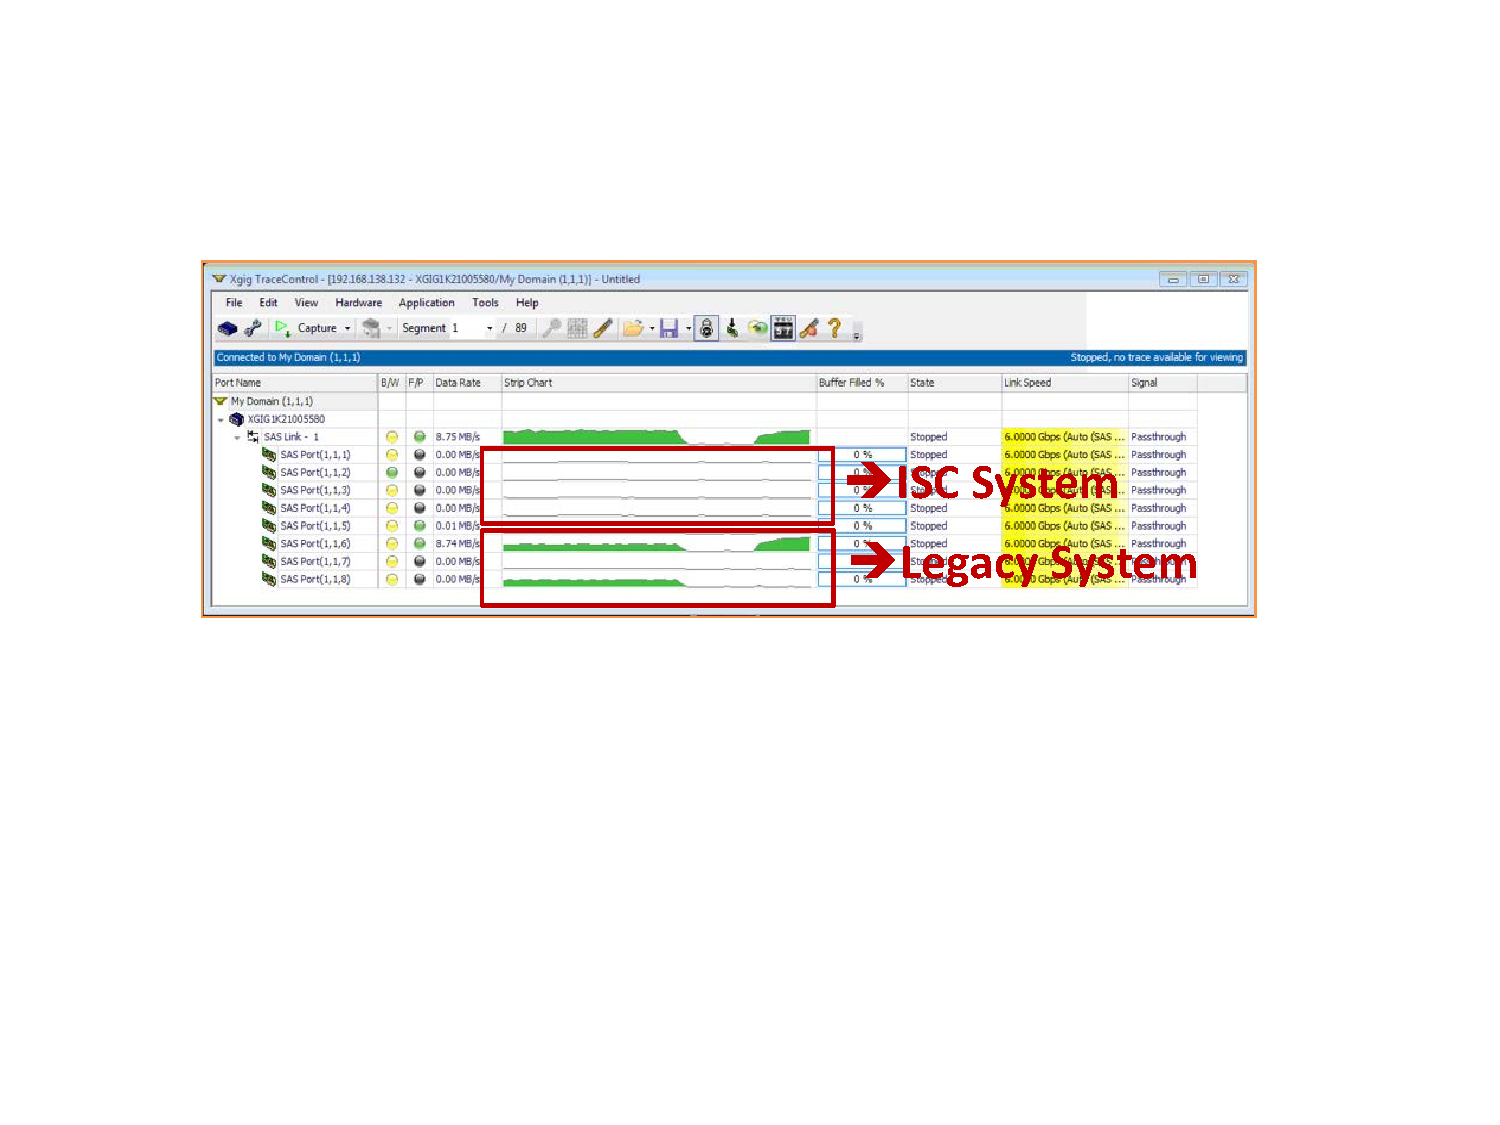
\includegraphics[width=0.99\columnwidth]{figures/Bus_Analyzer.pdf}
\end{tabular}
  \caption{The amount of data transfer from a device to a host. The upper most green bar corresponds to the total amount of data for both systems.}
  \label{fig:Bus_Alanyzer}
 \end{figure}


Figure~\ref{fig:Bus_Alanyzer} shows the amount of data transferring from a device (SSD) to a host system and we captured this with our 12Gbps SAS/SATA bus analyzer~\cite{BusAnalyzer:JDSU:techspec}. For this study, we set up two Hadoop systems (i.e., our proposed ISC Hadoop system and typical Hadoop system with SSDs) and connect them to the bus analyzer. Then, we run the same Hadoop application with identical data on both Hadoop systems at the same time. As shown in the figure, both exhibit a huge difference between our ISC model (upper rectangle) and the traditional CPU-centric computing model (lower rectangle). This clearly presents that the ISC system does not (or very rarely) transfer data to the host system for computation, while the legacy CPU-centric system keeps loading all the data to the host system (that is, host DRAM). All the main benefits of the ISC system originate from this factor.


Even though the main idea of ISC has been already proposed and implemented in the context of Hard Disk Drives (HDDs), it was not successfully adopted because of the still very limited computational capabilities of HDDs~\cite{Keeton1998,ActiveDisks:ASPLOS:1998}. However, the modern SSDs have been equipped with even stronger computing resources such as multi-core CPUs and DRAM so that people start to rethink of SSDs as another type of a computing unit, not just as a faster HDDs. 

SSDs typically provides a lot higher internal bandwidth (about 5$\times$ higher) than host I/O interface (SATA or SAS) bandwidth~\cite{SmartSSD:SIGMOD:2013,Minerva:De:2013}. The SSDs adopted for our ISC Hadoop system offers about 3.2GB/s of the aggregated internal bandwidth, while 750MB/s of host I/O interface bandwidth\footnote{\small Both are theoretical bandwidths and based on Samsung 6Gb SAS Enterprise SSD (400GB SLC).}. Thus, moving data from devices to a host results in a significant waste of the high internal bandwidth. 
In addition, the low I/O latency inside SSDs is another noticeable factor. A regular I/O operation is affected heavily by the entire OS stack which introduces extra overheads (e.g., context switching, interrupt, file system overhead, etc). However, the internal I/O latency in SSDs can avoid those OS software overheads. These factors implies that \emph{I/O intensive applications can significantly benefit from the ISC model} because, unlike CPU-centric computing system, ISC systems can make the best use of the high internal bandwidth and low internal I/O latency. 

SSDs, in general, are equipped with low power processors not only to save energy consumption but also to lower manufacturing costs. This factor results in an ambivalent value of ISC computing model. That is, the low power processor such as ARM processors can help ISC applications save energy consumption. On the other hand, it implies \emph{CPU computation intensive applications are not favorable to our current ISC computing model}.


\begin{figure}[htbp]
  \centering
  \begin{tabular}{ccc}
 %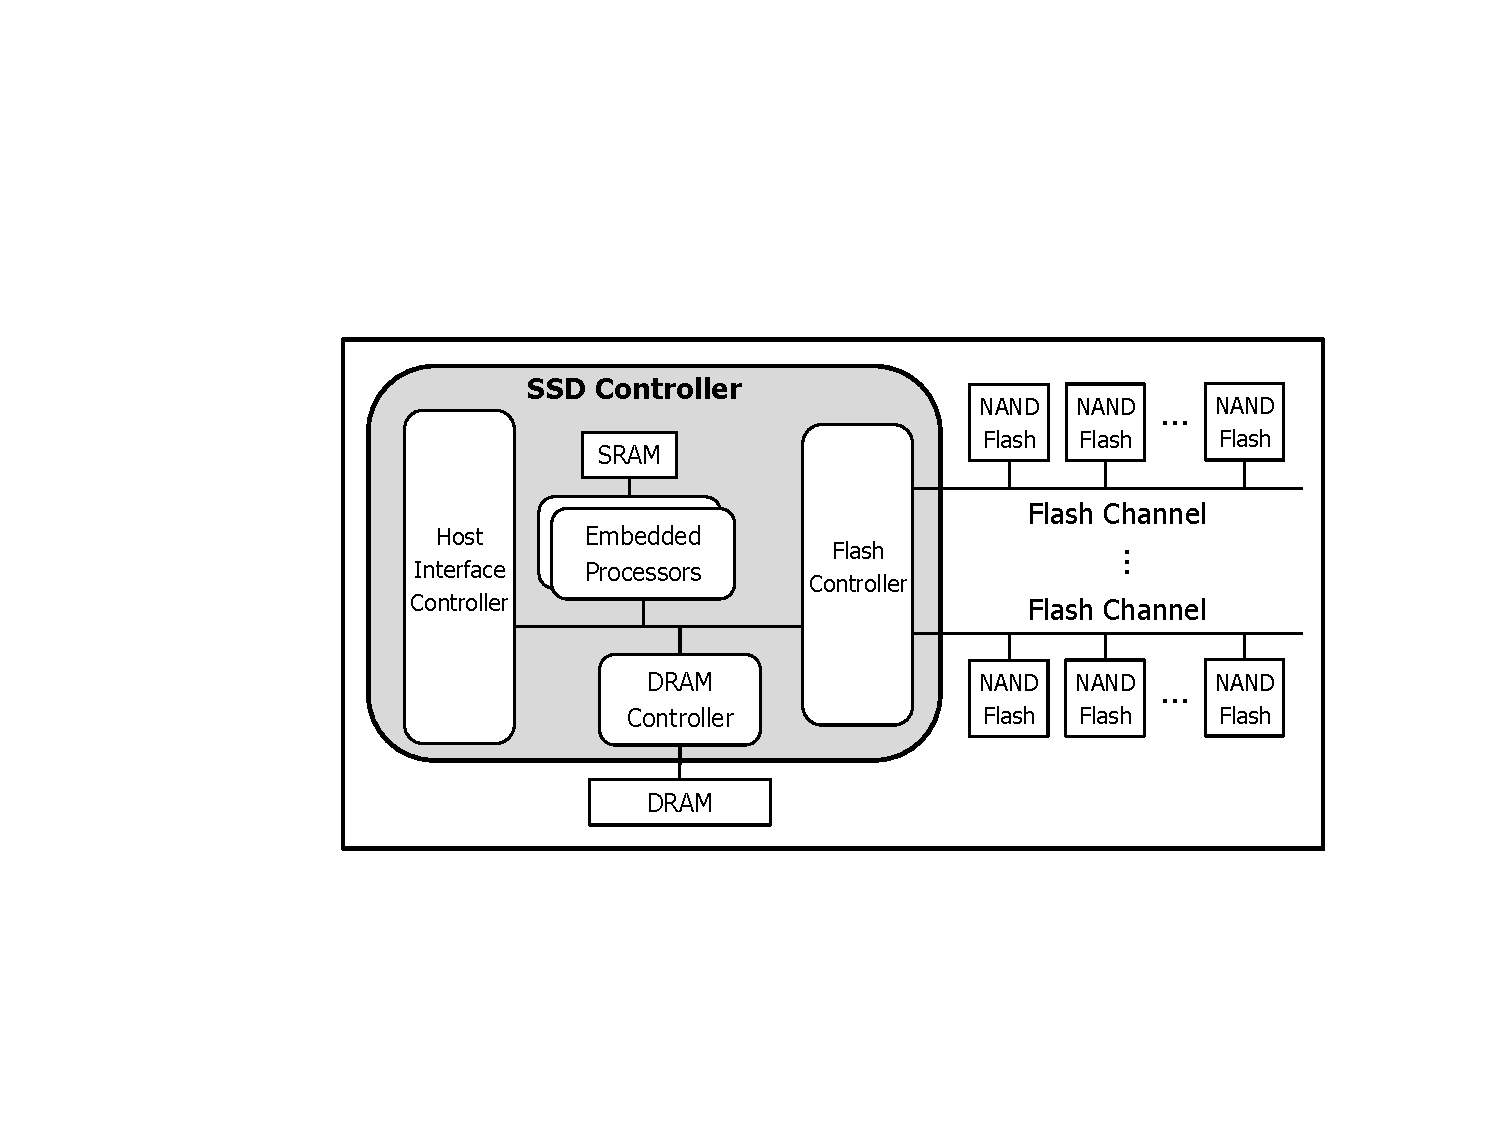
\includegraphics[width=0.95\columnwidth]{figures/SSDInternals.pdf}
 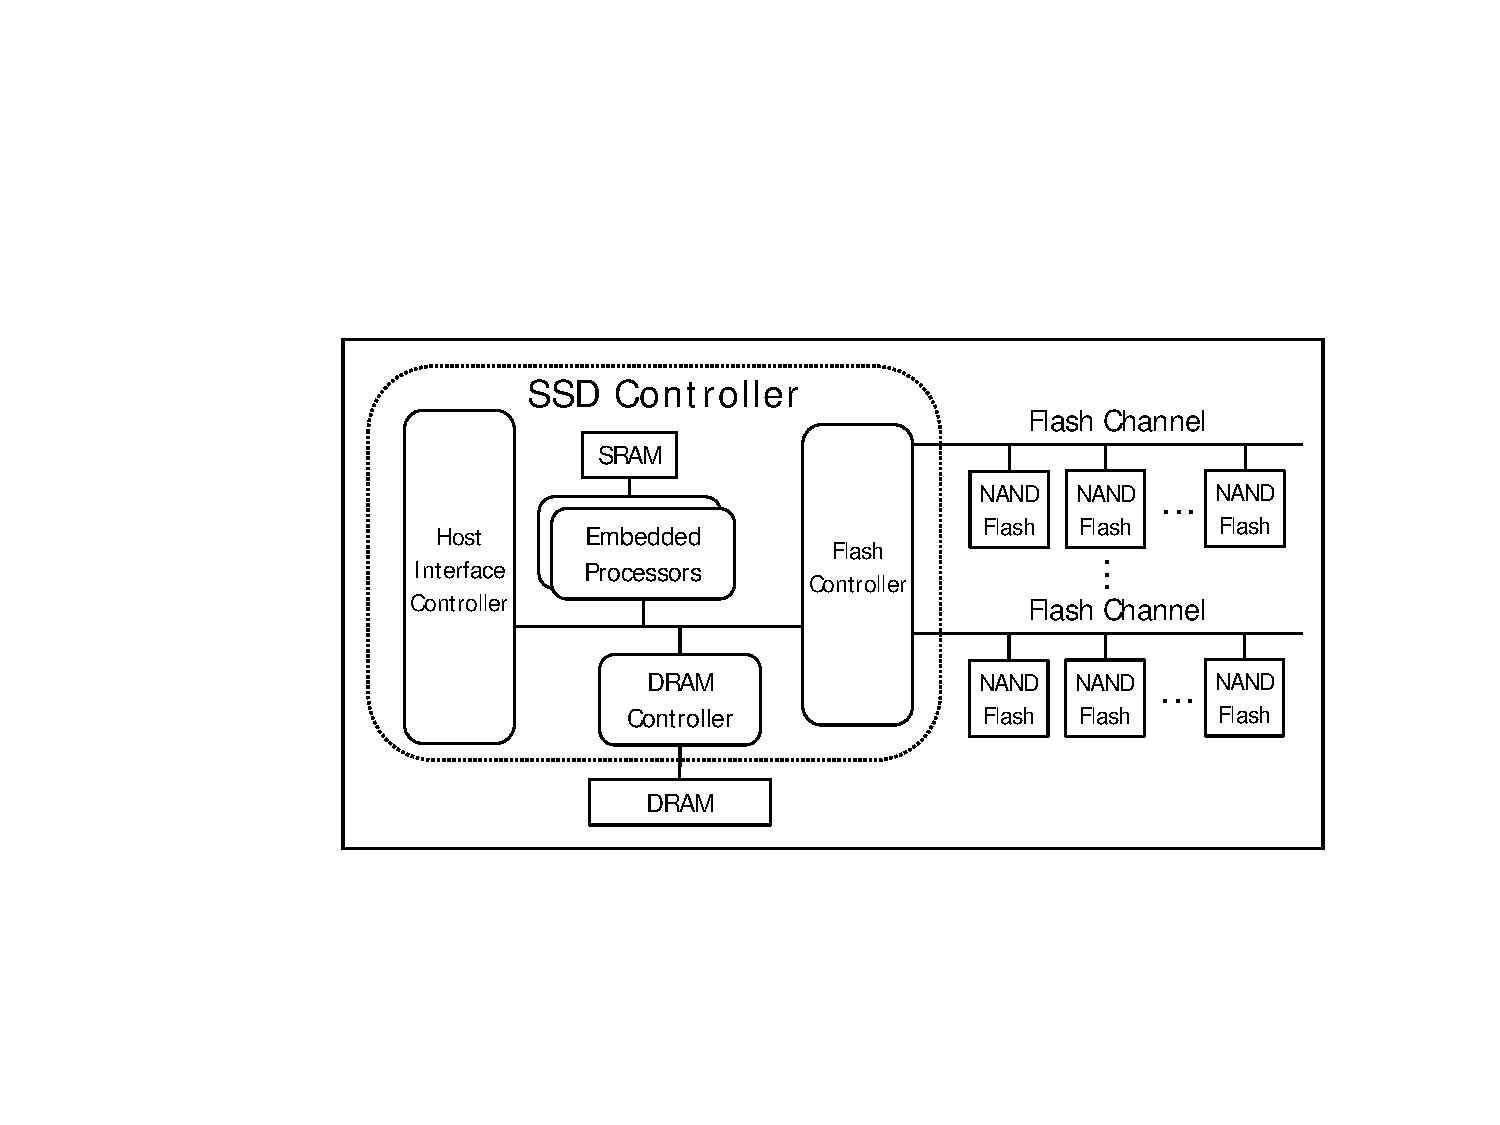
\includegraphics[width=0.99\columnwidth]{figures/ISC_HW_architecture.pdf}
\end{tabular}
  \caption{ISC hardware architecture}
  \label{fig:SSDInternals}
 \end{figure}


\subsubsection{ISC Hardware Architecture}\label{sec:SSDhw}
Figure~\ref{fig:SSDInternals} represents the hardware architecture of the modern SSD. The hardware architecture of our ISC SSD device is identical to regular SSDs.
%SSDs typically provides a lot higher internal bandwidth (about 5$\times$ higher) than host I/O interface (SATA or SAS) bandwidth~\cite{SmartSSD:SIGMOD:2013}. The SSDs adopted for ISC Hadoop framework offers about 3.2GB/s of the aggregated internal bandwidth, while 750MB/s of host I/O interface bandwidth\footnote{\small Both are theoretical bandwidths and based on Samsung 6Gb SAS Enterprise SSD (400GB SLC).}. This implies that moving data from devices to a host results in a significant waste of the high internal bandwidth. Unlike CPU-centric computing system, ISC systems can make the best use of this high internal bandwidth. 

An SSD is largely composed of NAND flash memory array, SSD controller, and (device) DRAM. The SSD controller is subdivided into four main subcomponents: host interface controller, embedded processors, DRAM controller, and flash controller.
The host interface controller processes commands from interfaces (typically SAS/SATA or PCIe) and distributes them to the embedded processors. Commands come from a user through the host I/O interface and the common interfaces are implemented by the host interface controller.
The embedded processors receive the commands and pass them to the flash controller. More importantly, they run SSD firmware codes for computation and execute Flash Translation Layer (FTL) for logical-to-physical address mapping~\cite{JSA:FTL:2009,CFTL:MASCOTS:2011}. Typically, the processor is a low-powered 32-bit processor such as an ARM processor. Each processor can have a tightly coupled memory (i.e., SRAM) to store performance-critical data or codes. Each processor can access DRAM through the DRAM controller. The flash controller controls data transfer between flash memory and DRAM.

%For data transfer between flash memory and DRAM, the Flash Controller, also called Flash Memory Controller (FMC), is adopted. The FMC runs Error Correction Code (ECC) and supports Direct Memory Access (DMA) functionality.

%The NAND flash memory package (also called chip) is persistent storage media and each package consists of one or more dies. The die is the smallest unit that can independently execute commands or report status. Each die contains one or more planes (usually one or two). Identical or concurrent operations can take place on each plane, although with some restrictions. Each plane subdivides into a number of blocks which are the smallest erase unit, and finally each block is composed of many pages (typically 64 or 128 pages)which are the smallest read/write unit.
The NAND flash memory package is the persistent storage media and each package is subdivided further into smaller units that can independently execute commands or report status.
An SSD is also equipped with a large size of DRAM for buffering data or storing metadata of the address mapping. All the flash channels share access to the DRAM. Thus, data transfer from the flash channels to the DRAM needs to be serialized~\cite{SmartSSD:SIGMOD:2013}.


%The Smart SSD ecosystem consists of both hardware (Section~\ref{sec:SSDhw}) and software components (Section~\ref{sec:softArch}) to execute user-defined programs.





\subsubsection{ISC Software Architecture}\label{sec:softArch}

%Smart SSDs, unlike the traditional CPU-centric computing systems, enable ISC devices to play a major role in computation by offloading key functions of host systems into ISC devices. Since its hardware architecture is identical to the aforementioned modern SSDs shown in Figure~\ref{fig:SSDInternals}, this section describes our Smart SSD software architecture and key components as ISC devices.

This section describes the system architecture and software key components for our ISC ecosystem including host system and storage device. Figure~\ref{fig:SmartSSD_arch} represents our ISC software architecture composed of two main components: \emph{ISC firmware} inside the SSD and \emph{ISC host program} in the host system. The ISC host program communicates with the ISC firmware through ISC Application Programming Interfaces (APIs).




\begin{figure}[tbp]
%\vspace{-5mm}
	\centering
		%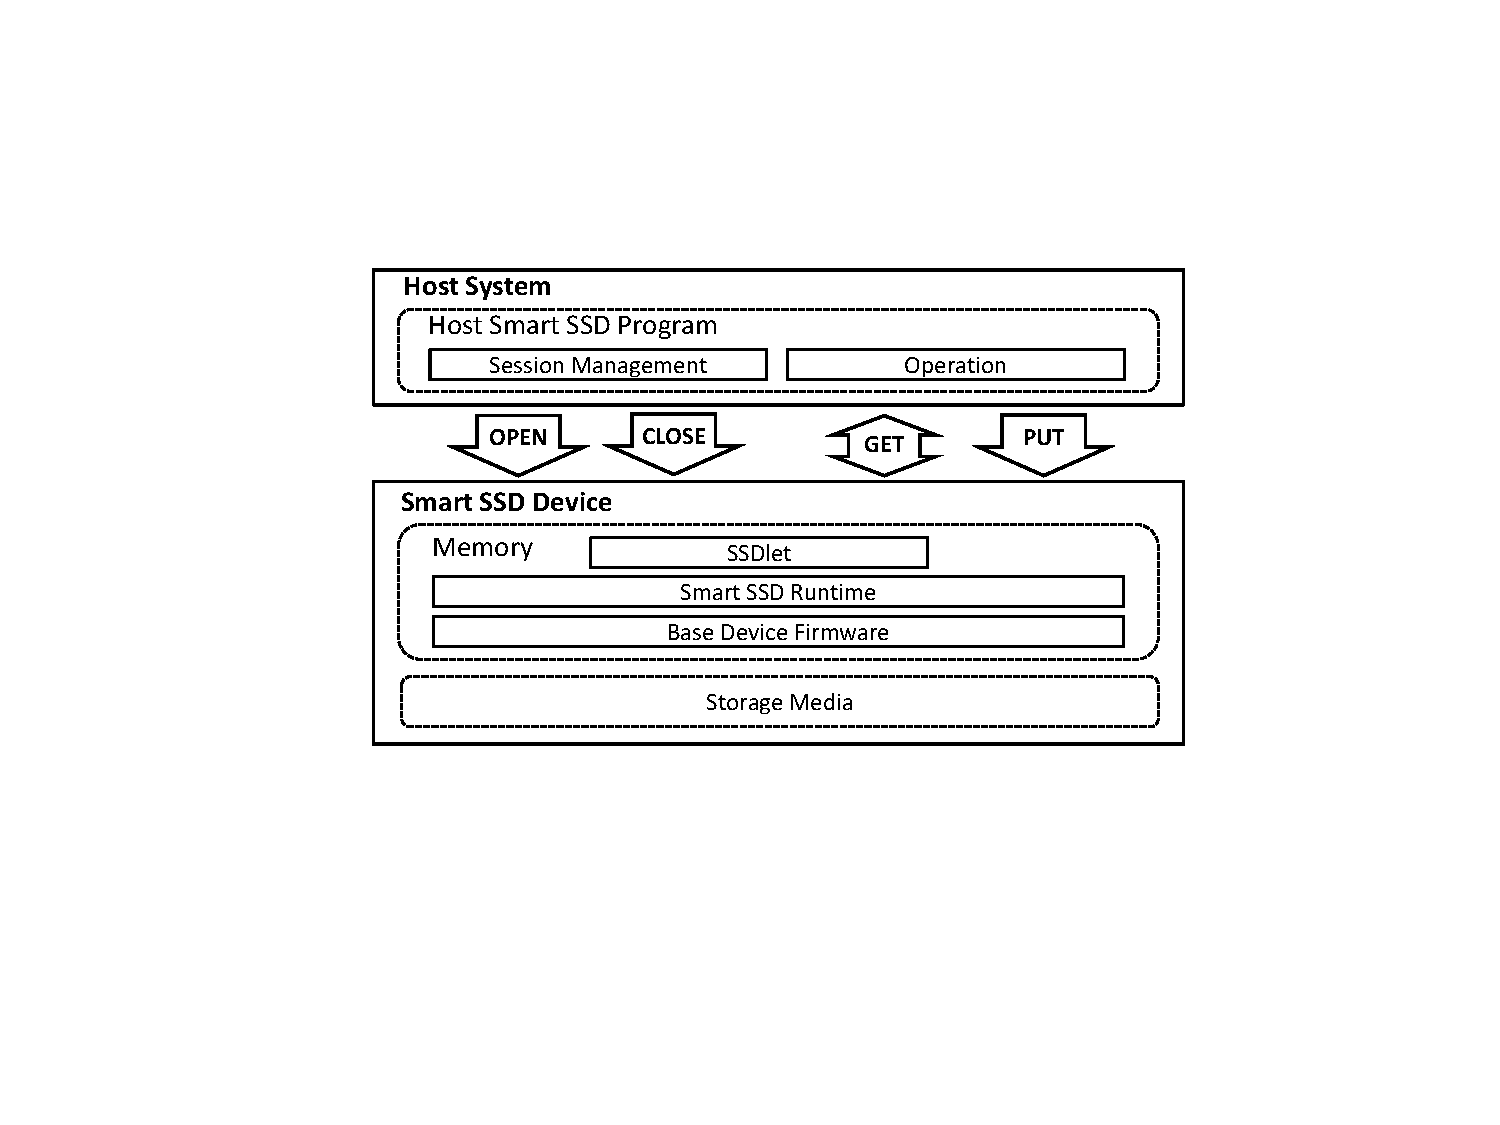
\includegraphics[width=0.95\columnwidth]{figures/SmartSSD_Architecture.pdf}
		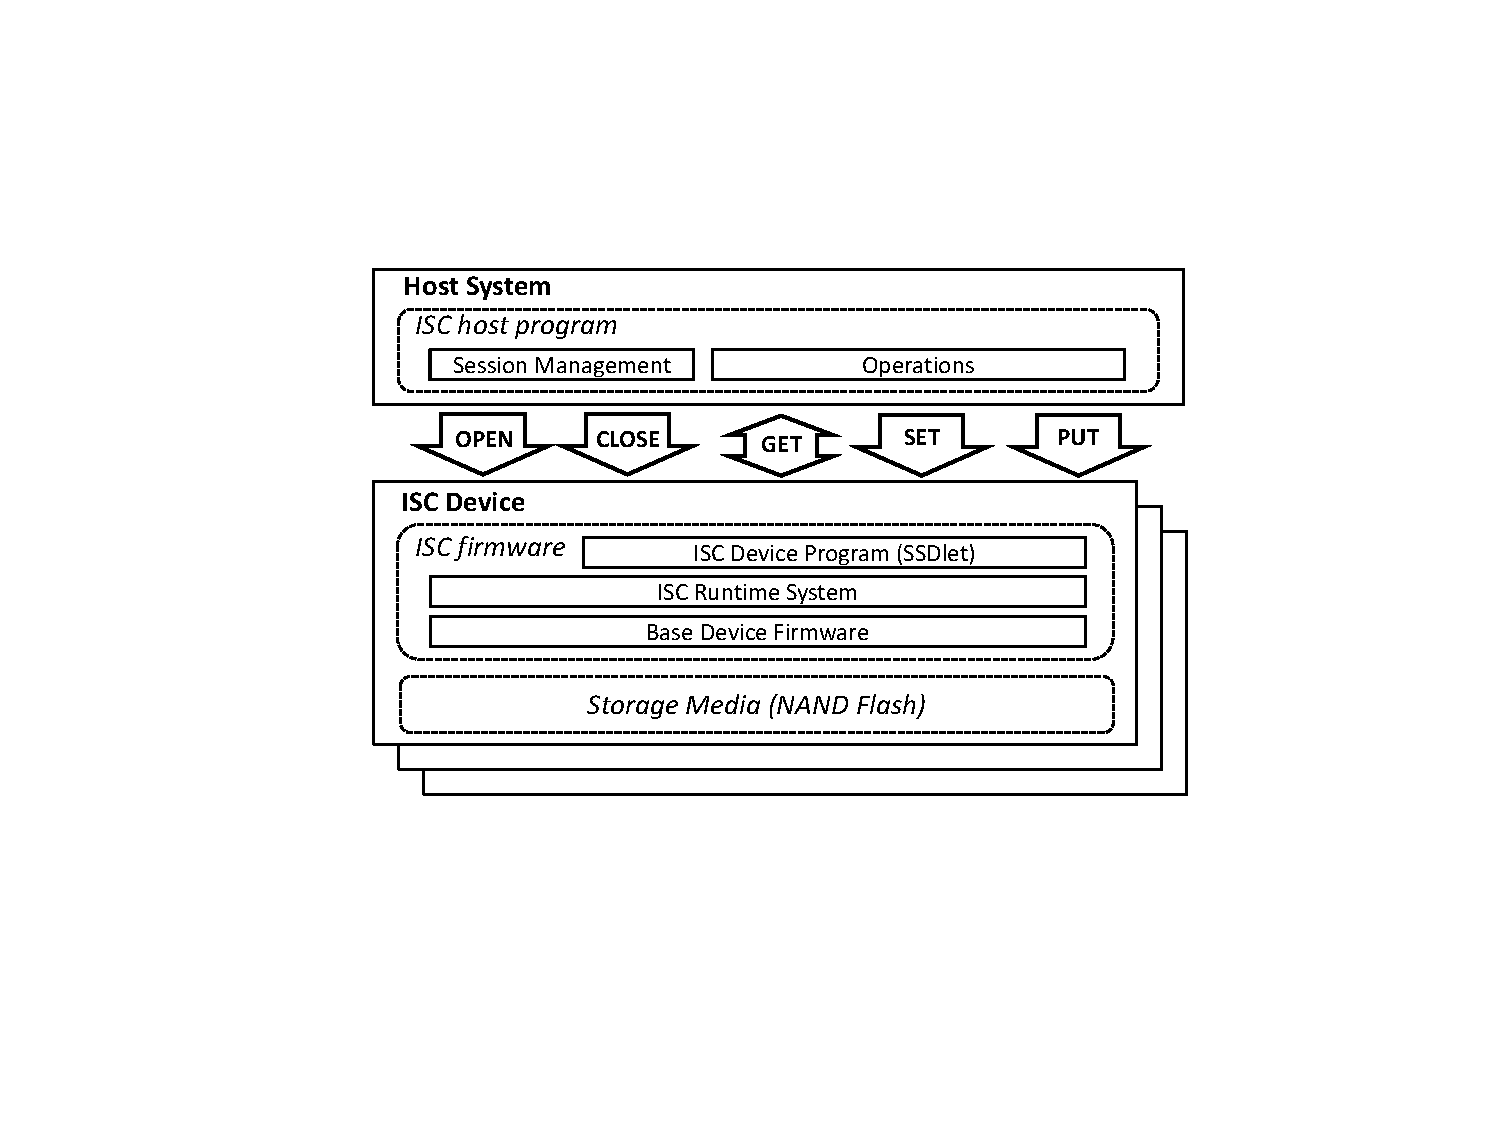
\includegraphics[width=0.99\columnwidth]{figures/ISC_SW_architecture.pdf}		
	\caption{ISC software architecture}
	\label{fig:SmartSSD_arch}
\end{figure}

%As illustrated in Figure~\ref{fig:SmartSSD_arch}, our Smart SSD consists of several key software components and it communicates with a Smart SSD host program via Smart SSD application programming models (APIs).

Since both a host system and an ISC storage device cooperatively compute data, we need to define two types of interactions (i.e., ISC host interface and ISC device interface) among a host, a device, and an ISC application. The ISC host interface is in charge of communication between the host and ISC devices to control ISP operations. The ISC device interface is on how the ISC runtime system in the storage device internally interacts with an ISC application in response to external inputs. A host ISC program implements the host interface logic, while a device ISC program (i.e., SSDlet) implements the device interface logic. We implement our ISC applications by using the ISC APIs.

The ISC firmware is subdivided into three sub-components: SSDlet, ISC runtime, and base device firmware.
An SSDlet is an ISC device program inside the SSD. It implements application logic and responds to the ISC host program. The SSDlet is executed in an event-driven manner by the ISC runtime system. An ISC runtime system connects the ISC device program with a base device firmware, and implements the library of ISC APIs. In addition, a base device firmware also implements normal I/O operations (read and write) of a storage device.

After the SSDlet is installed in the ISC device, a host system runs the ISC host program to interact with the SSDlet in the devices. This ISC host program consists largely of two components: a session management component and an operation component. The session component manages the lifetime of a session for ISC device applications so that the ISC host program can launch an SSDlet by opening a session to the ISC device. To support this session management, our ISC programming model provides two APIs, namely, OPEN and CLOSE. OPEN starts a session and CLOSE terminates a session. Once OPEN starts a session, the runtime resources such as memory and threads are assigned to run the SSDlet and a unique session ID is returned to the ISC host program. %This session ID must be associated to interact with the SSDlet afterwards. 
When CLOSE terminates the established session, it releases all the assigned resources and closes SSDlet associated with the session ID.

Once a session is established by OPEN, the operation component helps the ISC host program interact with SSDlet in an ISC device with GET, SET and PUT APIs. This GET operation is used to check the status of SSDlet and receive output results from the SSDlet if the results are ready. This GET API implements the polling mechanism of the SAS/SATA interface because, unlike PCIe, such traditional block devices cannot initiate a request to a host such as interrupts. 

Aside from the existing OPEN, GET, and CLOSE APIs, \emph{we implemented two more APIs: SET and PUT}. The SET operation delivers the new ISC metadata information (e.g., starting LBA, data length, etc.) from a host to an ISC device within a session. This SET API is very useful to process multiple non-contiguous data within one session. Without the SET API, we had to re-open another session after closing the previous session, which causes an extra overhead. PUT is also newly implemented to internally write data to the NAND flash media without help of a local file system. This API is useful to store the intermediate data during ISC processing.


\subsection{Hadoop MapReduce Framework}\label{sec:searchEngineArch}

\begin{figure}[htbp]
  \centering
  \begin{tabular}{ccc}
 %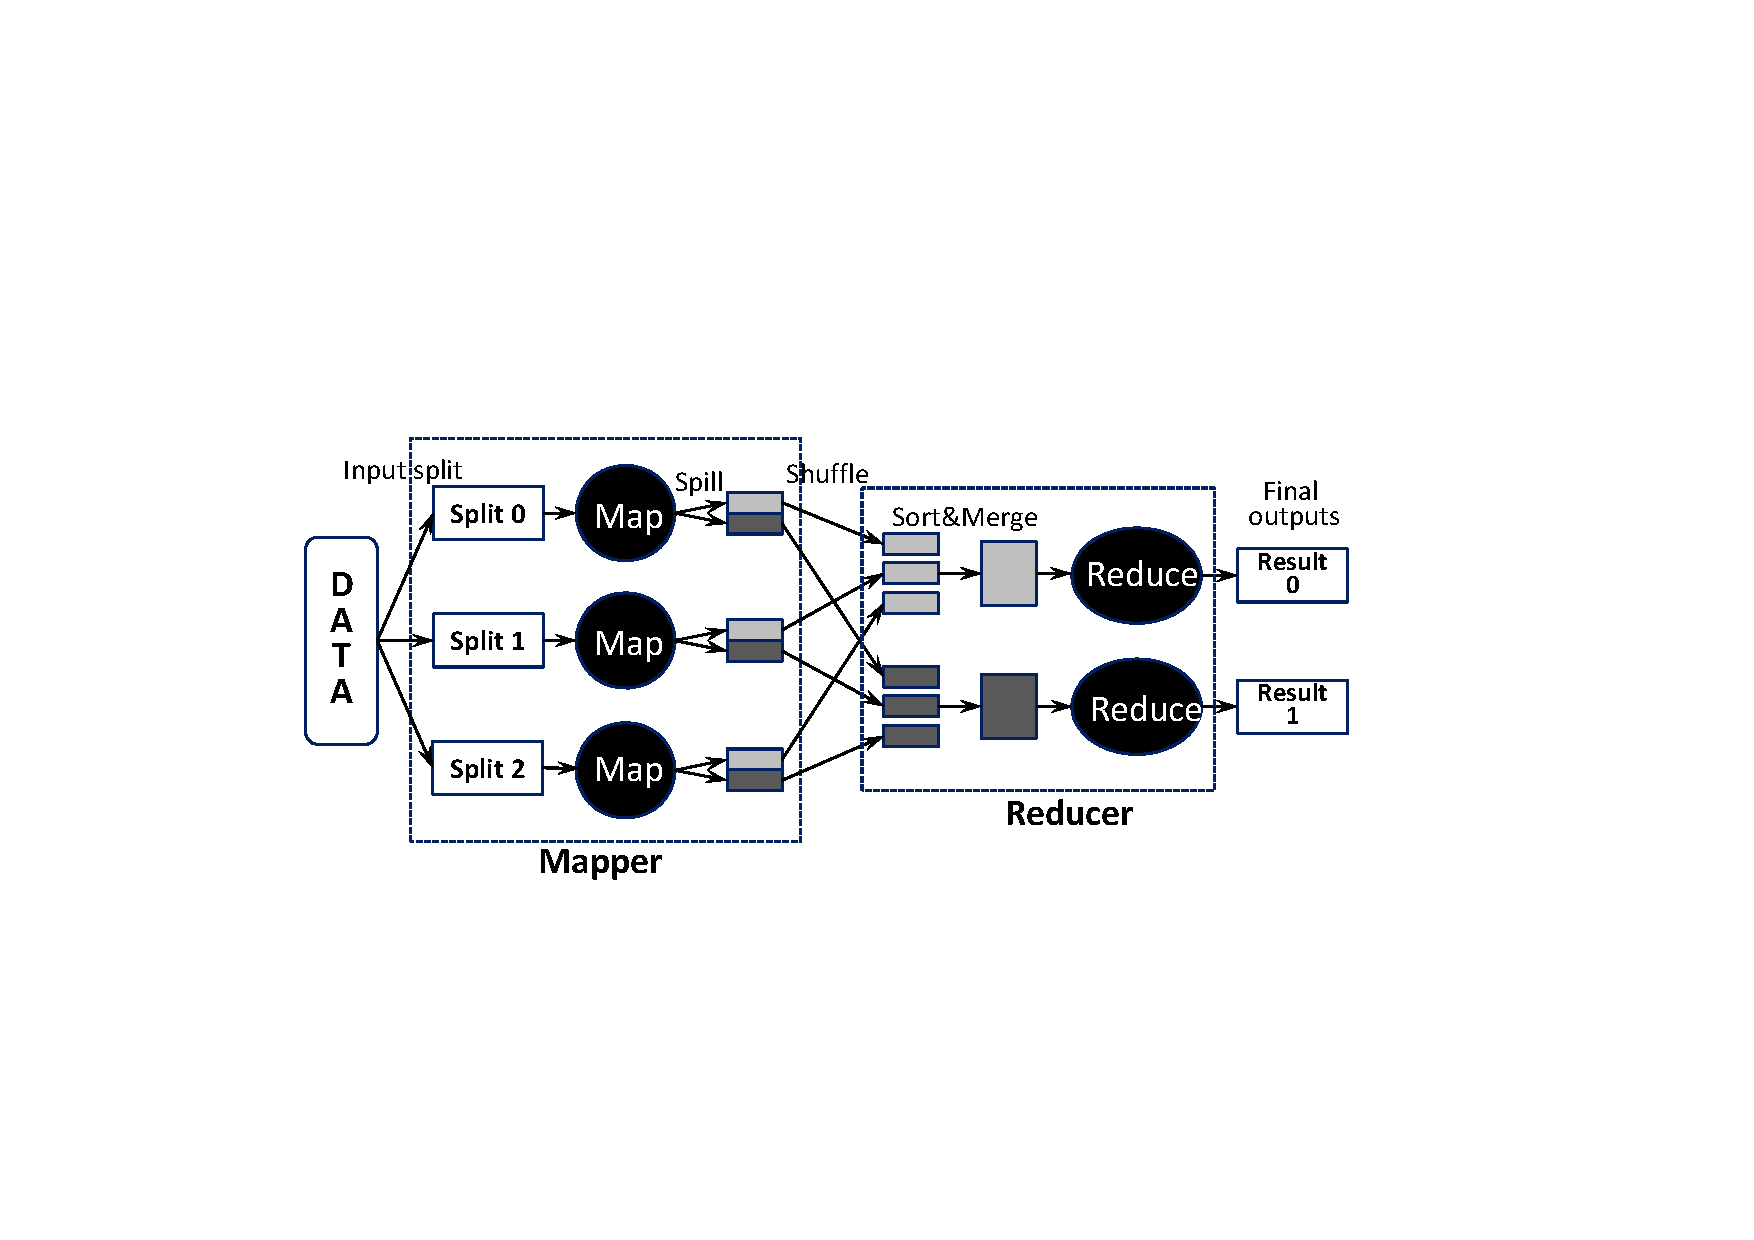
\includegraphics[width=0.99\columnwidth]{figures/HadoopMR_mono1.pdf}
 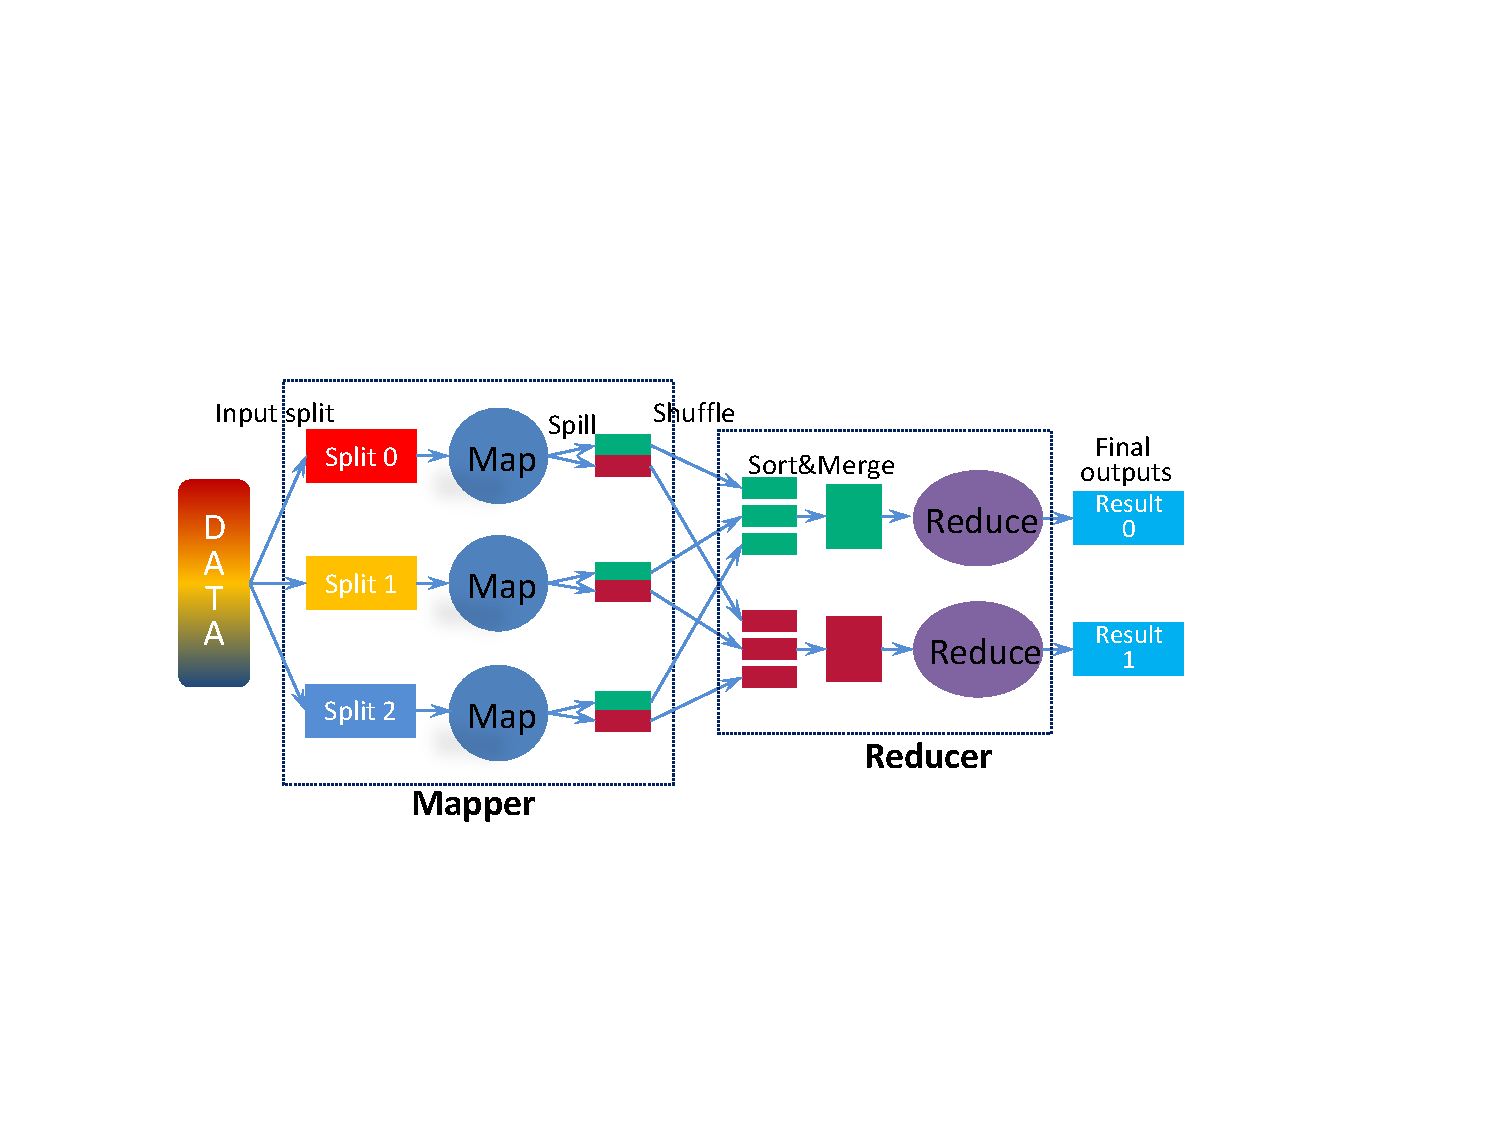
\includegraphics[width=0.99\columnwidth]{figures/HadoopMR.pdf}
\end{tabular}
  \caption{Hadoop MapReduce Framework}
  \label{fig:HadoopMR}
 \end{figure}



Hadoop is an open source implementation of the original MapReduce parallel programming model and system designed by Google~\cite{MapReduce:OSDI:2004}. MapReduce is a software framework for distributed processing of large data sets on commodity clusters~\cite{HadoopMapReduce:ACM:2010}. The Hadoop MapReduce framework leverages a distributed file system called the Hadoop Distributed File System (HDFS) which is an open source implementation of Google Distributed File System (GFS)~\cite{GFS:SOSP:2003}. The main design of the HDFS is heavily optimized for manipulating very large files with streaming data access patterns (i.e., write-once, read-many patterns). A MapReduce job consists of both Map and Reduce tasks, and one complete MapReduce job is subdivided largely into three phases: Map, Shuffle, and Reduce phase.

As illustrated in Figure~\ref{fig:HadoopMR}, at the beginning of a Hadoop MapReduce processing, Hadoop splits large input data into a set of data chunk of a predefined size (by default 64MB). Each split data is fed to each Map task which is executed in parallel on many physical machines. The Map tasks apply the Map function to its own input split data and generate a set of output data (i.e., intermediate key-value pairs). If a user implemented an optional combine function, Map tasks apply this combine function to each key-value pair list at this moment. Now, each Map task partitions the intermediate data (key-value pairs) into the number of Reduce groups. 
We offload this Map function into the ISC device.

Once all Map tasks are successfully completed, Hadoop MapReduce framework transfers the Map outputs to the Reducers as inputs, which is known as the Shuffle. Each Reduce task requests one intermediate data file from each Map task and starts to merge them on the basis of the intermediate key. Someone think of this Shuffle phase simply as a part of Reduce phase and they call it a 'copy' step in the Reduce phase.

After all Reduce tasks copy their own intermediate data, they start to sort and merge them first. Then they apply a Reduce function to the sorted data and emit the final output for each Reducer. Reduce tasks write their final outputs to a file with Hadoop Distributed File System (HDFS).






%\textcolor{red}{Need more description on namenode, datanode, job tracker and task tracker.}

%\textcolor{red}{For general search engines, many other techniques, e.g., caching, early termination. These works are orthogonal to us. We can also benefit from that.}


%
\section{Smart SSD Architecture}\label{sec:ssdArch}

%In-storage computing (ISC, for short) is a new computing paradigm and has recently attracted notable attention. Unlike the traditional CPU-centric computing systems, it enables ISC devices to play a major role in computation by offloading key functions of host systems into ISC devices. This paradigm reflects well a recent computing trend toward~\textit{'insurrection of peripheral devices'}. This section describes our Smart SSD architecture and key components as ISC devices.

%SSD In-Storage Computing (ISC) is a new computing paradigm and has recently attracted notable attention. Unlike the traditional CPU-centric computing systems, it enables ISC devices to play a major role in computation by offloading key functions of host systems into ISC devices. This paradigm reflects a recent computing trend toward \emph{near-data processing}~\cite{Balasubramonian14}. This section describes our Smart SSD architecture and key components as ISC devices.

Smart SSDs, unlike the traditional CPU-centric computing systems, enable ISC devices to play a major role in computation by offloading key functions of host systems into ISC devices. Since its hardware architecture is identical to the aforementioned modern SSDs shown in Figure~\ref{fig:SSDInternals}, this section describes our Smart SSD software architecture and key components as ISC devices.



\begin{figure}[htbp]
%\vspace{-5mm}
	\centering
		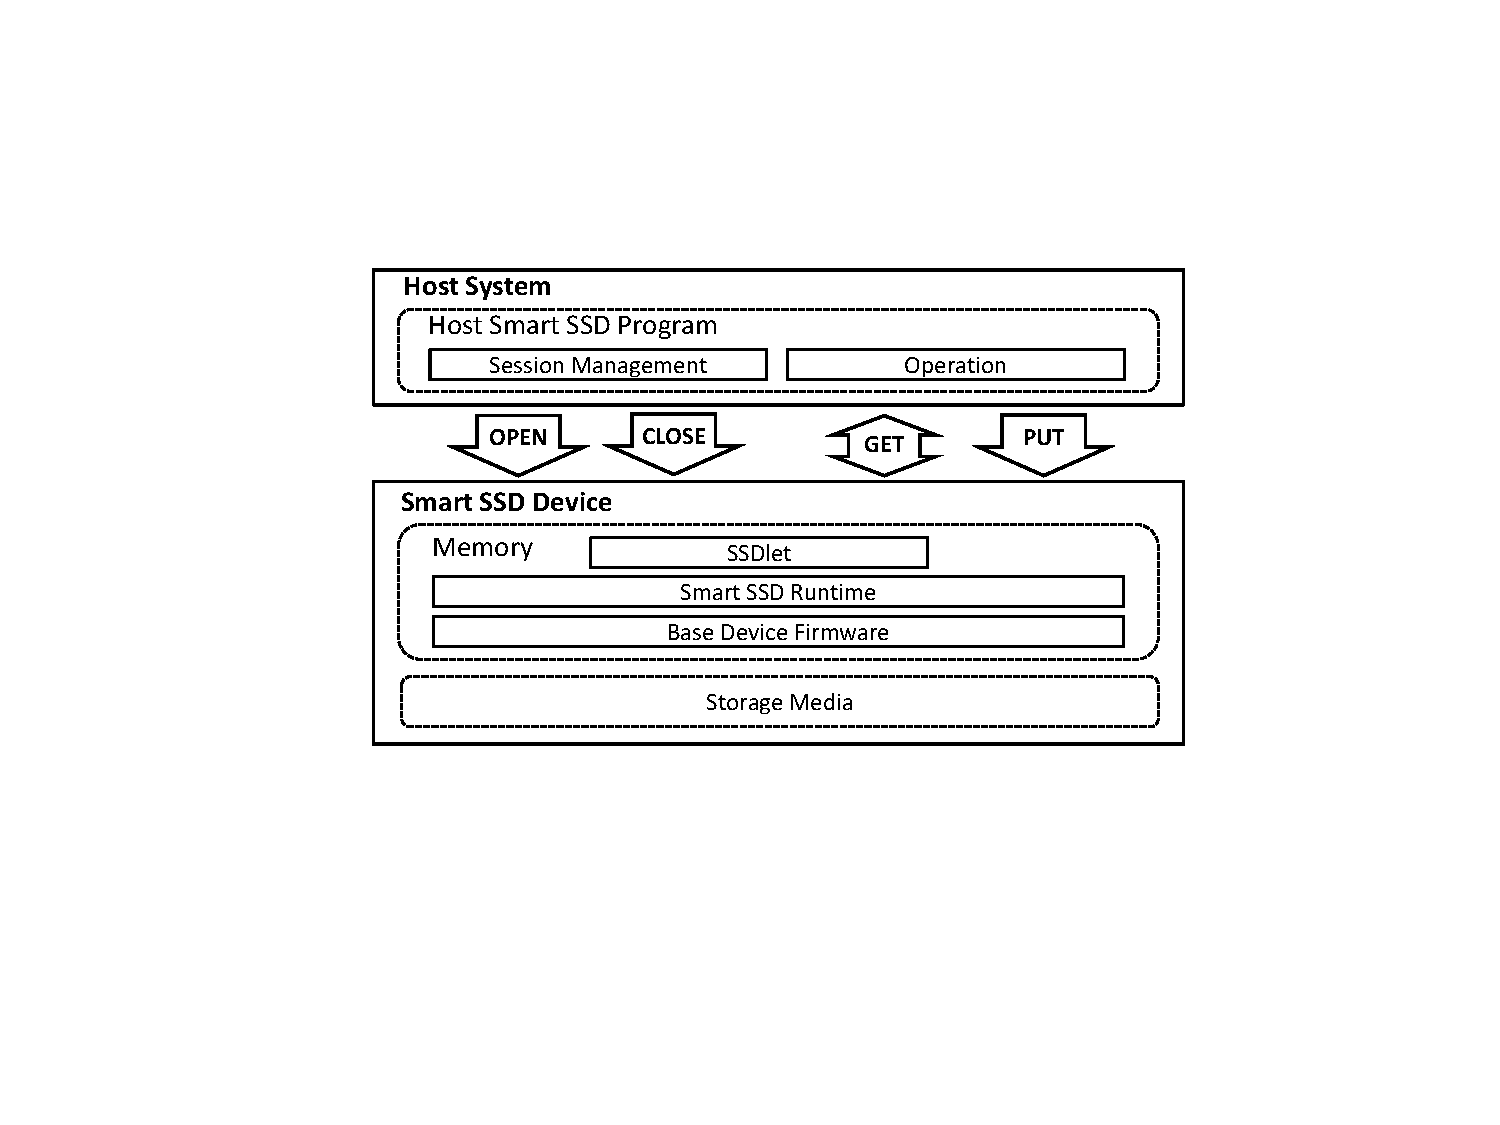
\includegraphics[width=0.9\columnwidth]{figures/SmartSSD_Architecture.pdf}
	\caption{\small Smart SSD Architecture}
	\label{fig:SmartSSD_arch}
\end{figure}

As illustrated in Figure~\ref{fig:SmartSSD_arch}, our Smart SSD consists of several key software components and it communicates with a Smart SSD host program via Smart SSD application programming models (APIs).


An SSDlet is a Smart SSD program in an ISC device. It implements application logic and responds to a Smart SSD host program. The SSDlet is executed in an event-driven manner by the Smart SSD runtime system. A Smart SSD runtime system connects the device Smart SSD program with a base device firmware, and implements the library of Smart SSD APIs. In addition, a base device firmware also implements normal I/O operations (read and write) of a storage device.

After an SSDlet is installed in the Smart SSD device, a host system runs the Smart SSD host program to interact with the SSDlet in the devices. This host program consists largely of two sections: a session management component and an operation component. The session component manages the lifetime of a session for Smart SSD applications so that the host Smart SSD program can launch an SSDlet by opening a session to the Smart SSD device. To support this session management, Smart SSD provides two APIs, namely, OPEN and CLOSE. Intuitively, OPEN starts a session and CLOSE terminates the existing session. Once OPEN starts a session, runtime resources such as memory and threads are assigned to run the SSDlet and a unique session ID is returned to the host Smart SSD program. Afterward, this session ID must be associated to interact the SSDlet. When CLOSE terminates the established session, it releases all the assigned resources and closes SSDlet associated with the session ID.

Once a session is established by OPEN, the operation component helps the host Smart SSD program interact with SSDlet in a Smart SSD device with GET and PUT APIs. This GET operation is used to check the status of SSDlet and receive output results from the SSDlet if the results are ready. This GET API implements the polling mechanism of the SAS/SATA interface because, unlike PCIe, such traditional block devices cannot initiate a request to a host such as interrupts. PUT is used to internally write data to the Smart SSD device without help from local file systems.





\section{ISC Hadoop MapReduce}\label{sec:design}
This section describes the system co-design of our In-Storage Computing model and Hadoop MapReduce framework.


%\textcolor{red}{1. architecture, 2. execution time analysis (mapper, shuffle, reduce, etc), why offload mapper, biggest portion, 3. flow chart explanation. Challenge added: mapping HDFS to a local file. 4. ISC is not always good solution. io intensive is the best app. cpu intensive is not good. 5. one node, multi real cluster. 6 multinodes Pseudo distributed mode, 7. data transfer comparision in bus anlyzer, 7. fully distributed mode on a single machine}




\begin{figure}[htbp]
%\vspace{-5mm}
	\centering
		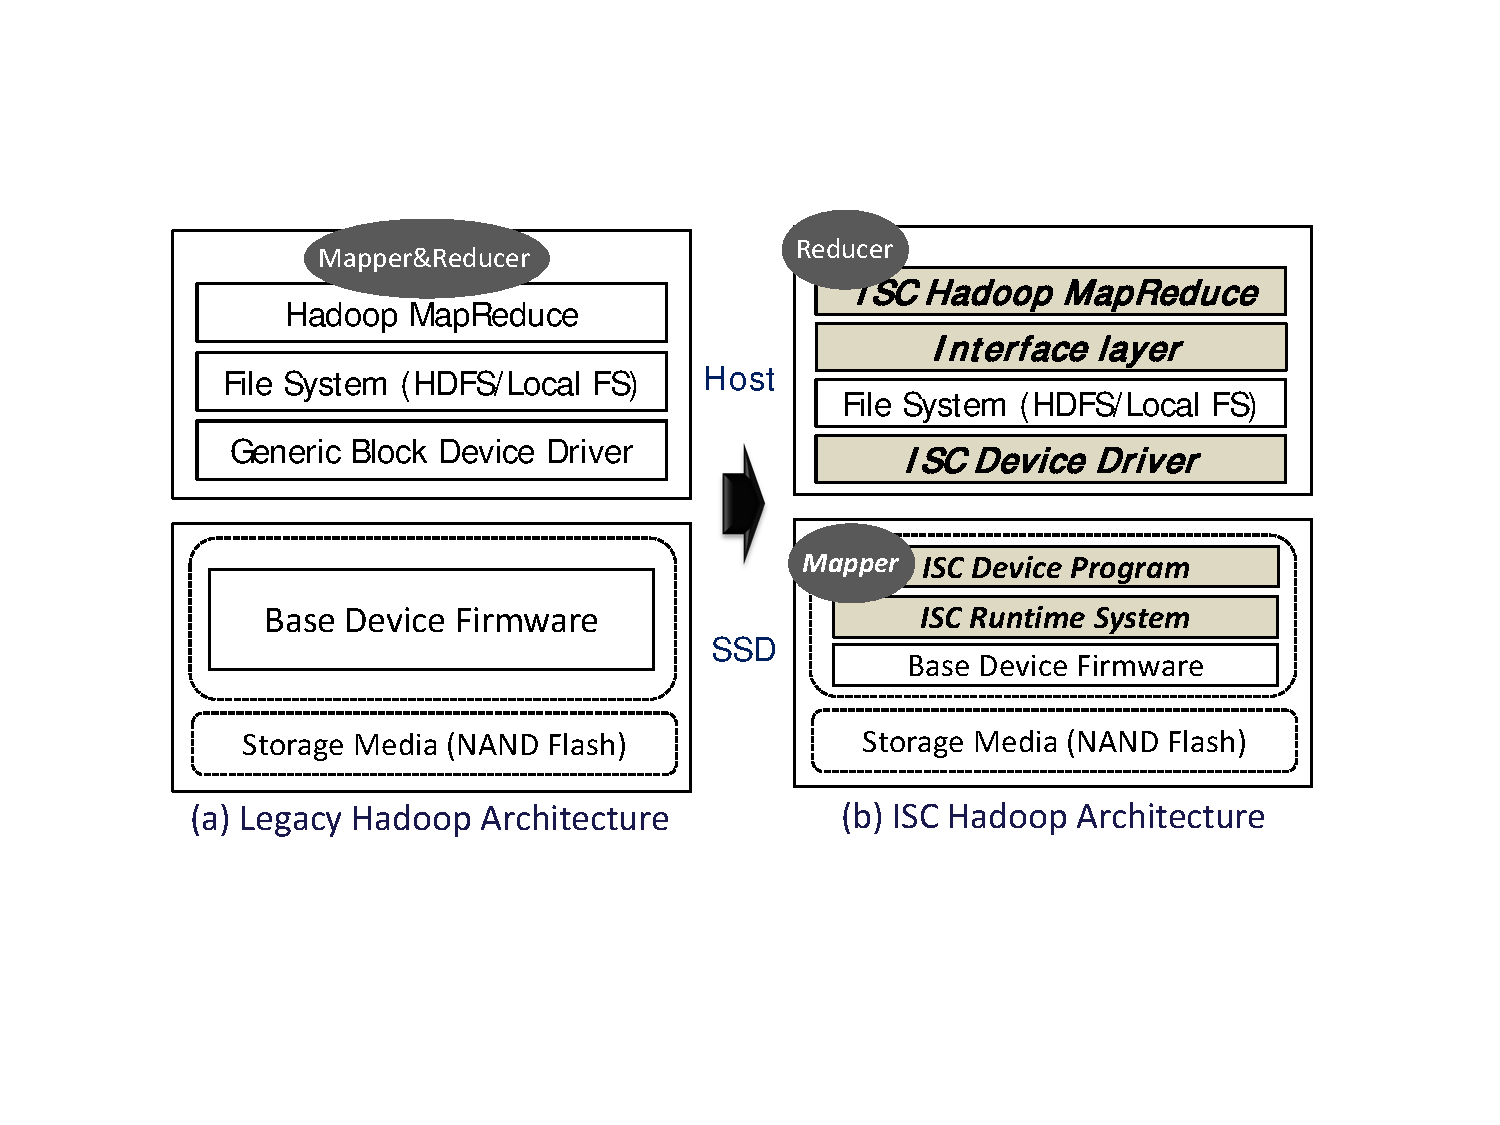
\includegraphics[width=1.0\columnwidth]{figures/ISC_Hadoop_architecture3.pdf}
	\caption{ISC Hadoop MapReduce architecture}
	\label{fig:ISC_Hadoop_arch}
\end{figure}


\subsection{System Architecture}\label{sec:designSpace}
Figure~\ref{fig:ISC_Hadoop_arch} shows an overall system architecture of our ISC Hadoop MapReduce framework. As explained, we offload the Mapper into an ISC device and implement the Mapper feature inside the real SSD firmware. Thus, a host Hadoop MapReduce system must be revised to collaborate with our ISC device thereby disabling Mapper features in the host system and implementing them inside SSD firmware (i.e., ISC device program). To support ISC functions, we also need to develop ISC engines (i.e., ISC Runtime System) on top of the existing base device firmware. The interface layer plays a role of an agent in communication between the host Hadoop MapReduce system and our ISC MapReduce system. We suggest this software component to resolve two major design issues: discrepancy in system interfaces and discrepancy in data representation between the host and the ISC devices (these issues will be addressed in the subsection~\ref{subsubsec:data_represent} and~\ref{subsubsec:system_interface} in detail.).
Alongside of a generic SCSI block device driver, we implement a special SCSI command to trigger ISC features inside the SSD (ISC Device Driver). We do not touch both HDFS and a local file system. So, our ISC Hadoop MapReduce system seamless supports all existing Hadoop features.   
%Moreover, to integrate our ISC Hadoop MapReduce model to the existing Hadoop MapReduce framework, we change Hadoop MapReduce components accordingly in the host for an ISC computing model, and develop an ISC device driver for the communication between the host system and our ISC device.

We first explore our work on a single Hadoop machine to verify our idea and concept, and then extend our design to Hadoop clusters of multiple nodes.


\begin{figure}[htbp]
%\vspace{-5mm}
	\centering
		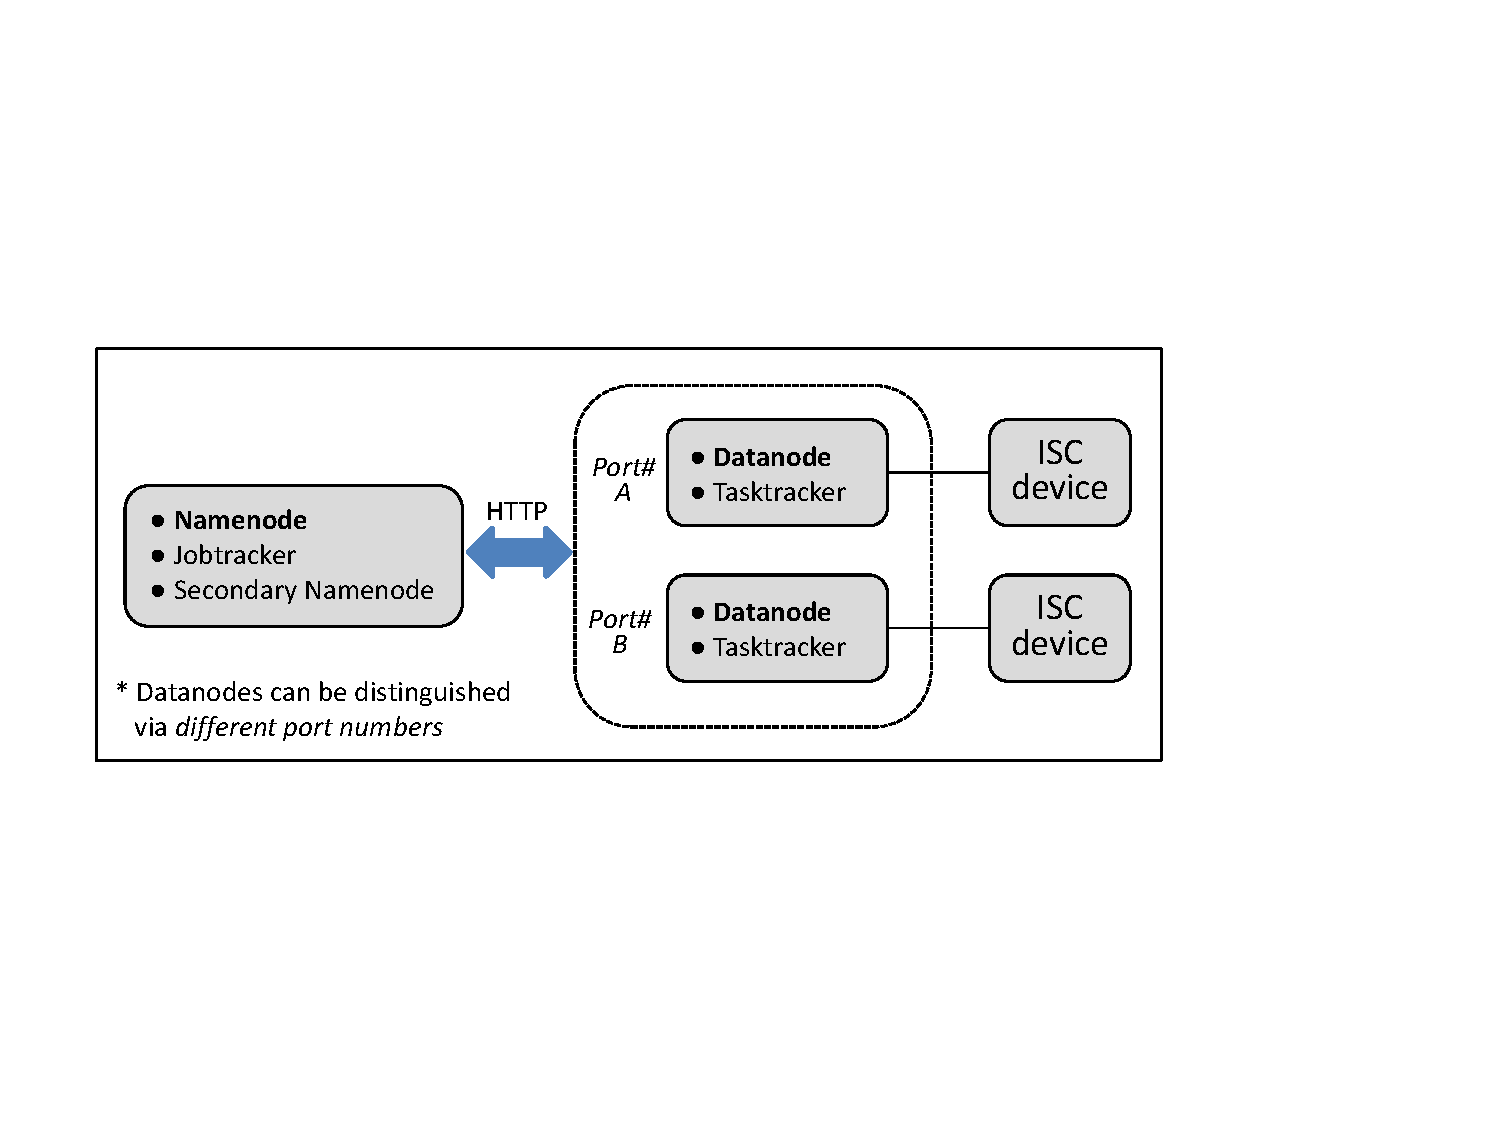
\includegraphics[width=1.0\columnwidth]{figures/Single_node_architecture.pdf}
	\caption{ISC Hadoop configuration on a single node: a fully distributed mode on a single machine}
	\label{fig:ISC_single_node_config}
\end{figure}

\subsubsection{A Single Node}\label{subsubsec:singlenode}
There are typically three ways to install and configure Hadoop: a local (standalone) mode, a pseudo distributed mode, and a fully distributed mode. In the standalone mode, all Hadoop components (i.e., namenode, jobtracker, datanode, tasktracker, secondary namenode) run in a single Java process (i.e., JVM instance) and this mode does not use HDFS. In the pseudo distributed mode, Hadoop runs all the components as separate Java processes and uses HDFS. This serves as a simulation for fully distributed Hadoop clusters but it runs \emph{a single instance of datanode on a single machine} only. The fully distributed mode runs on clusters of multiple machines with a master (plays namenode and job tracker. Optionally secondary namenode) and slaves (plays datanodes and tasktrackers) concept~\cite{MapReduce:Tutorial}. 

As described, basically it is impossible to run Hadoop in a fully distributed mode on a local machine (i.e., \emph{multiple instances of datanode on a single machine}). We, however, install and configure Hadoop in the fully distributed mode on a single node with a workaround, which is very efficient to initially verify our proposed ISC Hadoop MapReduce framework. Figure~\ref{fig:ISC_single_node_config} illustrates this Hadoop configuration on a single node. We configure separate Hadoop configuration files for each datanode instance. For HTTP communication with the namenode, we assign different port numbers for each datanode instance, wherein each datanode connects with our ISC device. Thus, each datanode can be distinguished via different port numbers for communication with the datanode\footnote{\small This configuration is based on Hadoop 0.20.205 and we found the assignment of virtual IPs to each datanode instance did not work for this workaround in this Hadoop version.}. This workaround mode represents the fully distributed Hadoop clusters on a single node.
 % and we found this performed very well (all the experiments of this configuration will be described in our experiment section in detail).



\subsubsection{Clusters: Multiple Nodes}\label{sec:multinodes}
The aforementioned single node configuration represents well the main features of the distributed Hadoop clusters on a local machine. Based on this observation, we extend our ISC Hadoop MapReduce framework to real Hadoop clusters. We set up the clusters of 5 nodes and separate a namenode from other datanodes (i.e., 1 namenode and 4 datanodes) to completely eliminate its performance overheads from the datanode. We initially start our study with one datanode and gradually increase the number of datanode to four on our clusters. Since we found meaningful and predictable performance results (that is, almost linear performance increase), we did not set up the bigger Hadoop clusters (please refer to our experiment results).


\begin{figure}[htbp]
%\vspace{-5mm}
	\centering
		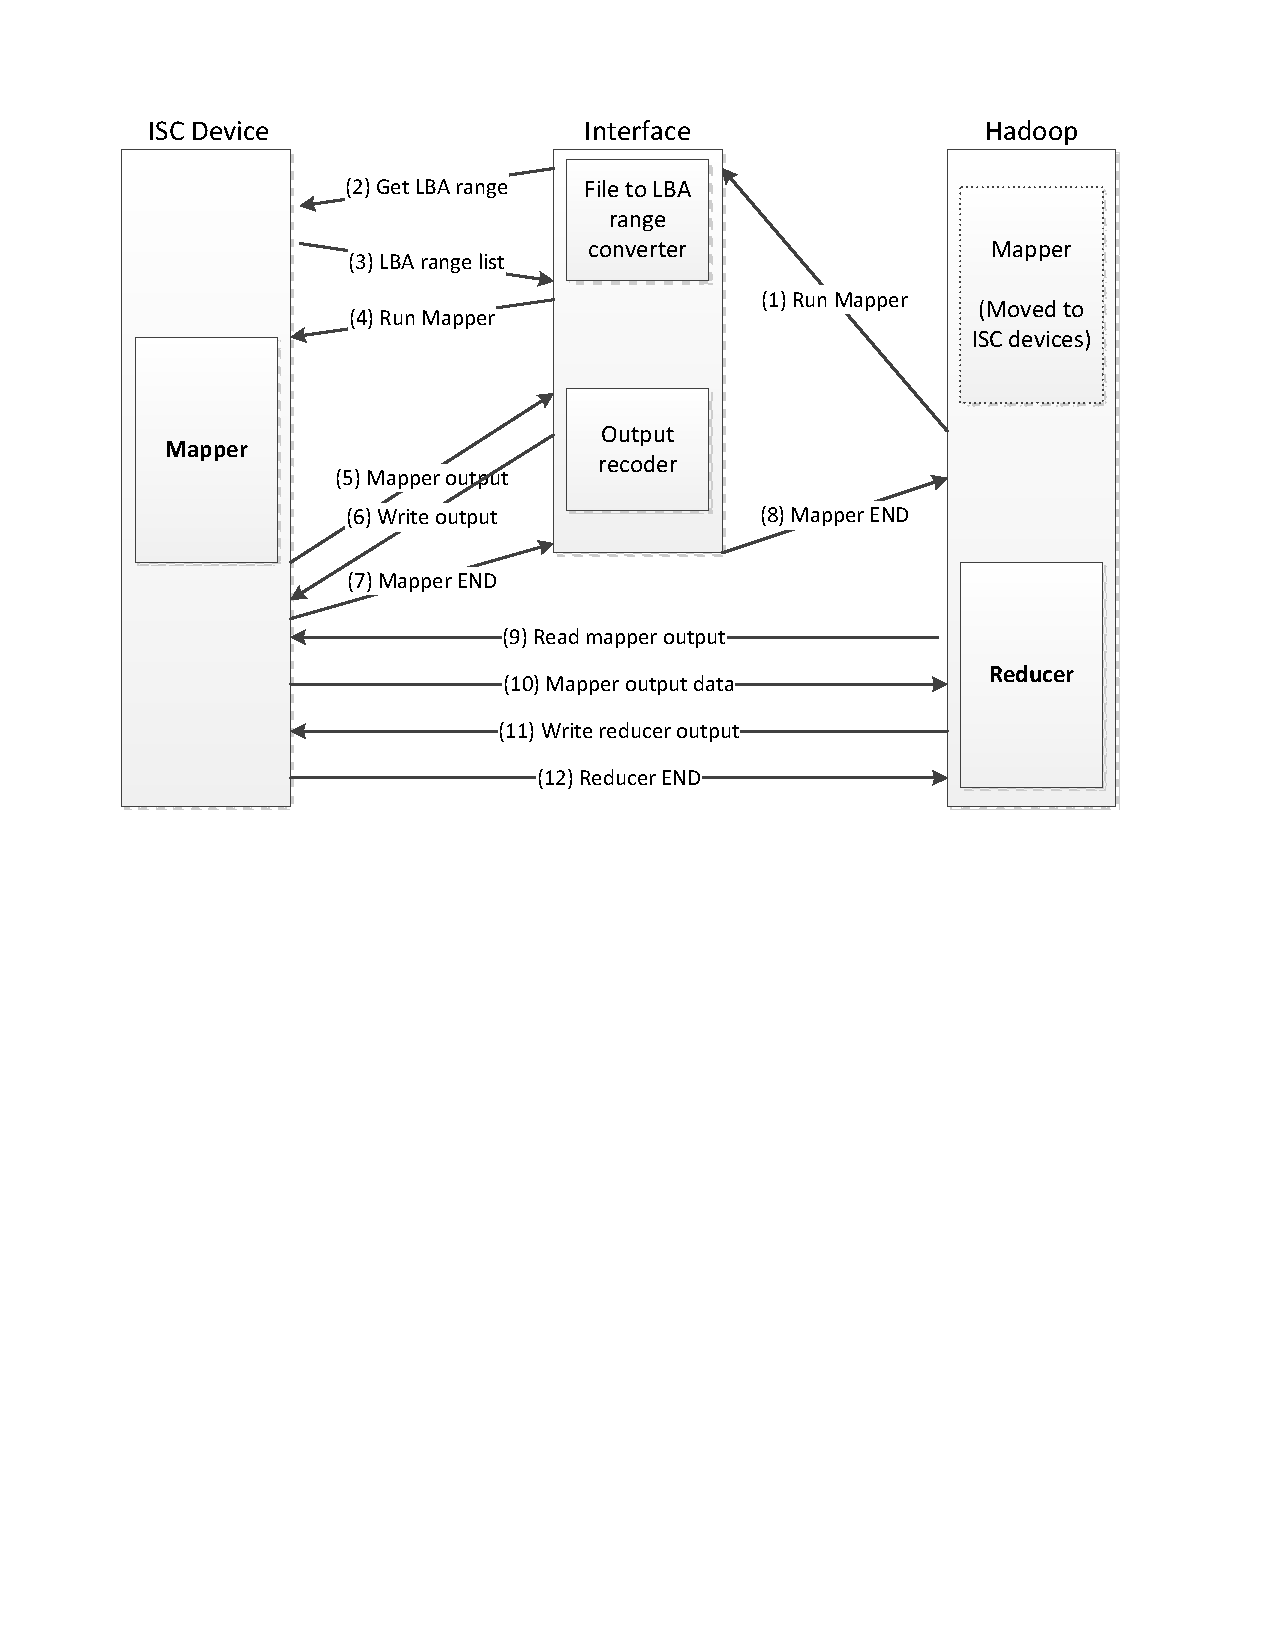
\includegraphics[width=0.98\columnwidth]{figures/ISC_Hadoop_Flowchart.pdf}
	\caption{ISC Hadoop MapReduce workflow}
	\label{fig:ISC_Hadoop_flow}
\end{figure}




\subsection{Workflow}\label{sec:workflow}
Figure~\ref{fig:ISC_Hadoop_flow} depicts our ISC Hadoop MapReduce workflow. Once a Hadoop application runs, our ISC Hadoop MapReduce framework does not directly run Mappers in the host system because they moved inside ISC devices. Instead, it first calls an interface component to communicate with ISC devices while delivering the input split data information (i.e., a file name of the input split) for ISC Map tasks. The interface runs its software component for converting each input split data (64MB) information to different data representation (i.e., LBA range information) for ISC devices. We found each input data of 64MB is generally split further into 2 or 3 smaller data chunks via an EXT4 file system. This means the software component in the interface (i.e., File to LBA range converter) delivers 2 or 3 LBA range lists to an ISC device for each Map task.
That is, the interface component calls Mapper inside the ISC device with these converted LBA range lists. After the Mapper receives all metadata information from the interface layer, it starts to execute a Map task. Once the Map task completes, the ISC devices return their Mapper outputs (i.e., intermediate results) to the interface layer to save them in the device (that is, the Mapper outputs are written with a local file system.). In fact, these Map output writing processes (Step 5 and 6) can be replaced with our new ISC API--PUT. Now, Reducers in the host can start to read the intermediate data as their input values and perform Reduce tasks. Finally all Map and Reduce tasks completes, our Hadoop system stores the final results with Hadoop Distributed File System (HDFS).



\subsection{Design Challenges}\label{sec:challenges}
This section addresses the challenging issues to design our ISC Hadoop MapReduce framework.

\subsubsection{Discrepancy in Data Representation}\label{subsubsec:data_represent}
To access data in a device, a host system can use file system information and so does the host Hadoop system by employing HDFS or local file systems such as EXT3/4. However, the device itself cannot rely on any file system information to access data inside its own device for ISC processing. This discrepancy in data representation between the host and the device causes an essential problem. This is the main reason the previous ISC work~\cite{SmartSSD:SIGMOD:2013,SmartSSDHadoop:MSST:2013} had no choice but to write their data to the raw device with 'dd' command by explicitly specifying their data locations (LBAs) from the beginning. This approach can temporarily evade this issue; but cannot resolve it. Consequently, it gives rise to other critical limitations on their systems. For instance, Kang et al. proposed a Hadoop MapReduce system leveraging ISC computation~\cite{SmartSSDHadoop:MSST:2013}. However, due to this challenging issue, their Hadoop system works only one local machine (i.e., no scalability) since it cannot support HDFS and local file systems. 
  
We fundamentally figure out this critical issue by developing a software component in the interface layer between the Hadoop system and ISC devices (please refer to the Figure~\ref{fig:ISC_Hadoop_flow}). This component is in charge of converting a file name into LBA range list information for the ISC device. Therefore, our proposed ISC Hadoop MapReduce system can seamlessly support the existing Hadoop features. For this, we first get a local file system information of each data split (64MB) from HDFS and convert it to LBA range lists. Then we deliver this information to ISC devices for Map tasks.


\subsubsection{Discrepancy in System Interfaces}\label{subsubsec:system_interface}
System interfaces between Hadoop framework in the host system and ISC device can be different. That is to say, Hadoop MapReduce framework in the host adopts Java programming language, while our SSD firmware for ISC processing uses C/C++ language. As a result, the host Hadoop system cannot directly communicate with ISC devices. To resolve this issue, we can think of two options: (1) running OS inside ISC devices and (2) adopting an interface layer. If an OS runs inside ISC device, it can also simply run JVM on top of the OS. This solution looks like very intuitive and may be able to eliminate our aforementioned challenge (i.e., discrepancy in data representation). However, this approach requires to consume extra ISC computing resources such as CPU and DRAM inside the device. Thus, unless the ISC device is a very specialized device with powerful computing resources, the first option will not be a good choice. 

As a matter of fact, since our ISC device is a typical commodity SSD without enough computing resources, we choose the second option. We, instead, put another interface layer between the Hadoop system and ISC devices by adopting Java Native Interface (JNI). Aside from the programming system interface between them, this interface layer plays two important roles in our ISC Hadoop System--first, as mentioned above, converting a file name to LBA range information, and second, writing the output data (i.e., intermediate data) of ISC Map tasks. For this, the host Hadoop system needs to deliver metadata information including an input split file name and an output file name of the intermediate data. The overhead of this extra interface layer is almost ignorable.


\begin{figure}[htbp]
%\vspace{-5mm}
	\centering
		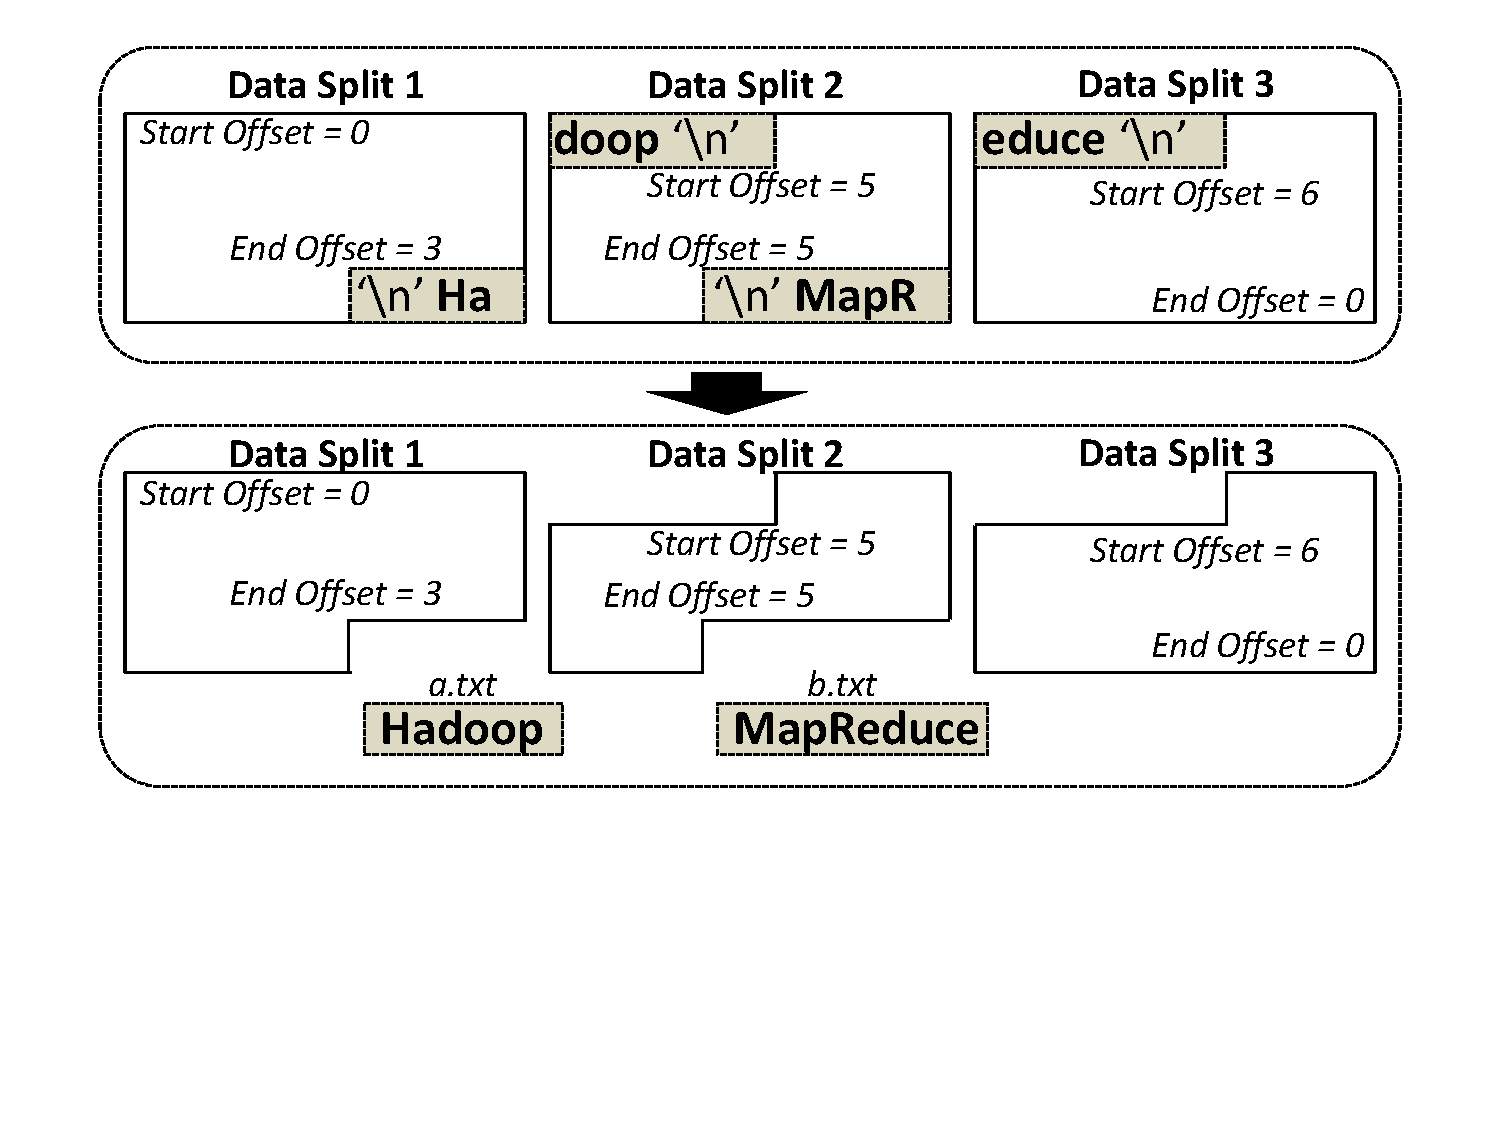
\includegraphics[width=1.0\columnwidth]{figures/Data_split_example2.pdf}
	\caption{A data split example}
	\label{fig:data_split_example}
\end{figure}

\subsubsection{Data Split}\label{subsubsec:data_split}
Hadoop Distributed File System (HDFS) splits large input data into a chunk of 64MB by default~\cite{TomWhite:HadoopDefinitiveGuide:2012}. This input split process raises another critical problem in ISC Hadoop system: data split. Figure~\ref{fig:data_split_example} illustrates this issue. Assuming a word data 'Hadoop' is stored in the large input data, HDFS may split the word 'Hadoop' into 'Ha' in one file of 64MB (i.e., Data Split 1) and 'doop' in another file of 64MB (i.e., Data Split 2) if the word inadvertently lies in the input split boundary. This does not causes any issue in a typical Hadoop system because HDFS in the host Hadoop system loads all input split data in the main memory and processes them in a streaming data access manner. However, since ISC Hadoop MapReduce framework basically does not move input data from devices to the host memory, this data split issue can cause a critical problem in the ISC Hadoop system. If the ISC device is equipped with such a capability that they can directly connect/communicate with each other like Ethernet-connected drives (e.g., Seagate's Kinetic HDD or HGST's Ethernet Drive~\cite{KineticHDD:Seagate:2014,EthernetDrive:HGST:2014}), we may be able to solve this issue with a naive way, but unfortunately, our ISC drive is not equipped with such a communication interface.

To resolve this, our ISC Hadoop system consults the host Hadoop system. If the host Hadoop system detects a split data\footnote{\small Host Hadoop system originally has a simple algorithm for this data split detection.}, it stores the split data (both Hadoop and MapReduce in the example) as a separate file respectively with a local file system. Then it converts the file name to LBA information by using the aforementioned software component and delivers the LBA information to the ISC device via the interface layer. To avoid inaccurate (i.e., duplicated) computation of that part inside ISC device, the host system provides the ISC device with another metadata information (that is, Start Offset and End Offset) for each data split. These offsets can be thought of as data lengths of each part including a delimiter, where the delimiter can be a carriage return, space, or tab, depending on the Hadoop applications. With the help of this metadata information, ISC Mapper can simply ignore processing all the data within the offset boundary in each data split chunk of 64MB.


%To resolve this, our ISC Hadoop system consults the host Hadoop system. If the host Hadoop system detects a split data\footnote{\small Host Hadoop system originally has a simple algorithm for this data split detection.}, it stores the split data as a separate file with a new file name. Then it converts the file name to LBA information and delivers the LBA information to the ISC device. To avoid inaccurate (i.e., overlapped) computation of that part inside ISC device, the host system should provide another metadata information regarding this overlapped part which should not be processed by ISC Mapper. For this, the host system provides its offset information to ISC device as metadata and the ISC device simply ignore all the data with the offset in the file.


\subsubsection{Feature Offloading}\label{subsubsec:feature_offloading}
%As discussed in the Section~\ref{sec:ISC_background} and previous work~\cite{SmartSSD:SIGMOD:2013,SmartSSDHadoop:MSST:2013}, our ISC model can be best utilized by the applications with the following characteristics: (1) I/O intensive (not heavily CPU intensive), (2) less data access per data page (i.e., 8KB flash memory page), and (3) a smaller amount of output data after data processing. I/O intensive applications can leverage a high internal bandwidth of SSDs and the less data access per data page is closely related to the low DRAM performance inside SSDs. If the ratio of the amount of data after processing vs. that of before processing is close to 1, these applications discard ISC performance gain thereby transferring the large final output data to a host system. Based on these observations, a database application best fits for those requirements~\cite{SmartSSD:SIGMOD:2013}. However, in this work, we explore another application for our ISC model: Hadoop MapReduce. 


The data precessing of Hadoop MapReduce framework is composed of Map and Reduce. Unlike a Map task that does not have any dependency among other tasks for its execution, a Reduce task is inherently dependent on other Map task executions. That is, a Reducer is required to collect output results of other Map tasks in its shuffle phase before a Reduce task starts. However, as we mentioned in the previous subsection~\ref{subsubsec:data_split} (Data Split), our ISC device is not equipped with such a communication capability, a host system should be in charge of collecting the intermediate data from each Mapper. Moreover, the host should redistribute the collected data to each ISC device for the Reduce execution. Not only can these processes incur unnecessary data movement traffic, but also can the ISC devices be overwhelmed by the overburden because typically an ISC device has very limited resources and both Mapper and Reducer, in general, are executed concurrently.

Many Hadoop MapReduce applications (not necessarily, but mostly) produce small amount of intermediate data after a Map task processes original big data. In addition, the Reduce task is subdivided into three major phases such as copy, sort, and reduce. Unlike a Map task, the Reduce task generally does not significantly lessen the data size of its output result after Reduce processing. This is not favorable to ISC framework~\cite{SmartSSD:SIGMOD:2013}. The sort can give rise to another unfavorable issue. Assuming a data size is bigger than an available DRAM space in an ISC device, it may have to issue tremendous NAND flash Write operations to store intermediate results, which has a critical impact on the life endurance of NAND flash memory~\cite{SSDDesignTradeOff:ATC:2008,IPL:SIGMOD:2007,HotData:MSST:2011,HotDataTrap:ACR:2013}. 

Based on these observations, we move Mapper to ISC devices, not Reducer, in the Hadoop MapReduce framework.



%Based on these observations, we move Mapper to ISC devices, not Reducer, in the Hadoop MapReduce framework. In general, many Hadoop MapReduce applications produce small amount of intermediate data after Map tasks process original big data. In addition, the Reduce task is subdivided into three major phases such as copy, sort, and reduce. Unlike a Map task, the Reduce task generally does not significantly lessen the data size of its output result after Reduce processing. This is not favorable to ISC framework~\cite{SmartSSD:SIGMOD:2013}. Moreover, the sort phase may require tremendous Write operations to store intermediate results, which has a critical impact on the life endurance of NAND flash memory~\cite{SSDDesignTradeOff:ATC:2008,IPL:SIGMOD:2007,HotData:MSST:2011,HotDataTrap:ACR:2013}. 



\subsection{Hadoop Applications}\label{sec:application}

As discussed in the Section~\ref{sec:ISC_background} and previous work~\cite{SmartSSD:SIGMOD:2013,SmartSSDHadoop:MSST:2013}, our ISC model can be best utilized by the applications with the following characteristics: (1) I/O intensive (not heavily CPU intensive), (2) less data access per data page (i.e., 8KB flash memory page), and (3) a smaller amount of output data after data processing. I/O intensive applications can leverage a high internal bandwidth of SSDs and the less data access per data page is closely related to the low DRAM performance inside SSDs. If the ratio of the amount of data after processing vs. that of before processing is close to 1, these applications discard ISC performance gain thereby transferring the large final output data to a host system. Based on these observations, a database application best fits for those requirements~\cite{SmartSSD:SIGMOD:2013}. In this work, we explore another application for our ISC model: Hadoop MapReduce. We can find many Hadoop applications with I/O intensive and generally they produce a smaller amount of final outputs after processing input data. 
However, unfortunately, Hadoop applications cannot meet the second characteristics (less data access per data page) since they have to read every single byte of all data to process them.

Admittedly, all Hadoop applications cannot benefit from our ISC Hadoop MapReduce framework. We now explore various Hadoop applications to choose an appropriate application for our experiment and discuss the rationale of the choice. 

For this Hadoop application study, we refer to Purdue MapReduce (PUMA) Benchmarks Suite~\cite{PUMA:Purdue:2012}. PUMA benchmark suite presents a broad range of Hadoop MapReduce applications (i.e., a total of 13 applications) exhibiting various application characteristics. We run PUMA benchmark on our Hadoop machine and analyze each application for our study. After the investigation, interestingly, we found many of the applications (7 out of 13 including wordcount) can be classified into a wordcount-like application. That is to say, (1) a processed data size is a lot smaller than an original data size, (2) average per-Mapper execution time is a lot longer than the average per-Reducer execution time (i.e., Mapper intensive), (3) their final results produce counting-related values, and (4) generally CPU intensive but not highly CPU intensive computation.

For the rest of applications, particularly, Terasort can be identified as a worst Hadoop MapReduce application for our ISC framework. Sorting applications including Terasort never reduce their processed data size, which is a very unfavorable characteristic to ISC framework~\cite{SmartSSD:SIGMOD:2013}. More critically, due to a limited DRAM resource inside our ISC devices, Terasort should generate an enormous number of flash write operations to temporarily store its intermediate data. This can critically impact NAND flash lifetime.
K-means clustering is another unfavorable MapReduce application for our ISC framework because an amount of transferring data is never reduced and instead it is even increased with extra information via many iterations. Moreover, relatively high CPU computation is required to calculate the cosine-vector similarity of a given data with all the centroids.

Based on our study, we choose Hadoop wordcount as our ISC application. As we mentioned above, this wordcount is a very representative application and many other benchmark programs (term-vector, inverted-index, histogram-movies, histogram-ratings, sequence-count, ranked-inverted-index, etc) retain a very similar characteristics to the wordcount application. Thus, we expect very similar results and implications to run other applications of them. Actually, several of them use the same input data as wordcount and exhibit even almost the same execution time as the wordcount based on our experiments. We could choose other ISC-favorable applications instead of the wordcount. However, its representativeness led us to go with it. 
The main goal of this work is not to run various Hadoop applications, but to verify our ISC Hadoop MapReduce framework and to explore its opportunities and challenges. Therefore, we leave implementing/running various applications including even ISC-unfavorable ones on top of our ISC framework as our future work.




%\textbf{Step S4: Execute list operations}. The main reason of loading inverted lists to the host memory is to efficiently execute list operations such as intersection. Thus, both steps S4 and S3 should be offloaded to Smart SSDs. This raises another question: what operation(s) could potentially benefit from Smart SSDs. In Lucene, there are three basic operations commonly used: list \textsf{intersection}, \textsf{union}, and \textsf{difference}. They are also widely adopted in many commercial search engines (e.g., Google advanced search\footnote{\small\url{http://www.google.com/advanced_search}}). We investigate each operation and set up a simple principle that the output size should be smaller than its input size. Otherwise, Smart SSDs cannot save any data movement. Let $A$ and $B$ be two inverted lists, and we assume $A$ is shorter than $B$ to capture the real case of skewed lists.
%\begin{itemize}%[noitemsep, topsep=2pt]
 % \item \textsf{Intersection}: The result size of the intersection is usually much smaller compared to each inverted list, i.e., $|A\cap B| \ll |A| + |B|$. E.g., in Bing search, for 76\% of the queries, the intersection result size is two orders of magnitude smaller than the shortest inverted list involved~\cite{Ding2011}. Similar results are observed in our real dataset. Thus, executing intersection inside SSDs may be a smart choice as it can save a lot of host I/O interface bandwidth.

 % \item \textsf{Union}: The union result size can be similar to the total size of the inverted lists. That is because $|A\cup B| = |A| + |B| - |A\cap B|$, while typically $|A\cap B| \ll |A| + |B|$, then $|A\cup B| \approx |A| + |B|$. Unless $|A\cap B|$ is similar to $|A| + |B|$. An extreme case is $A = B$, then $|A\cup B| = |A| = |B|$, meaning that we can save 50\% of data transfer. However, in general, it is not cost-effective to offload \textsf{union} to Smart SSDs.

 % \item \textsf{Difference}: It is used to find all the documents in one list but not in the other list. Since this operation is ordering-sensitive, we consider two cases: $(A - B)$ and $(B - A)$. For the former case, $|A - B| = |A| - |A\cap B| < |A| \ll |A| + |B|$. That is, sending the results of $(A - B)$ saves a lot of data transfer if executed in Smart SSDs. On the other hand, the latter case may not save much data transfer because $|B - A| = |B| - |A\cap B| \approx |B| \approx |B| + |A|$. Consequently, we still consider the \textsf{difference} as a possible candidate for query offloading.
%\end{itemize}

%\textbf{Step S5: Compute similarity and rank}. After the aforementioned list operations are completed, we can get a list of qualified documents\footnote{\small Lucene assumes the results are small enough to fit into main memory, thus, no any I/O involved.}. %Lucene assumes the results are small enough to fit into main memory.
%This step applies a ranking model to the qualified documents in order to determine the similarities between the query and these documents. This is because users are more interested in the most relevant documents. This step is CPU-intensive so that it may not be a good candidate to offload to Smart SSDs. However, it is beneficial when the result size is very large because after step S5, only the top ranked results are returned. This can save a lot of I/Os. From the design point of view, we can consider two options: (1) do not offload step S5. In this case, step S5 is executed at the host side; (2) offload this step. In this case, step S5 is executed by Smart SSDs.


%\begin{table}[htbp]\small
%\centering
%\begin{tabular}{l|c|c}\hline\hline
%&Non-Ranked & Ranked \\\hline
%\textsf{Intersection} & \ding{51} & \ding{51} \\\hline
%\textsf{Union} &\ding{55}  & \ding{51}\\\hline
%\textsf{Difference} & \ding{51}& \ding{51}\\\hline\hline
%\end{tabular}
%\caption{Design space}\label{tab:designSpace}
%\end{table}

%
\section{Implementation}\label{sec:implementation}
This section describes the implementation details of offloading the query operations into Smart SSDs. We discuss the implementation of intersection in Section~\ref{sec:intersection}, union in Section~\ref{sec:union}, and difference in Section~\ref{sec:difference}. Finally, we discuss the implementation of ranking in Section~\ref{sec:ranked}.

\textbf{Inverted index format}.
Inverted index is a fundamental data structure in Lucene as well as other search engines.
It is essentially a mapping data structure between query terms and inverted lists.
Each inverted list includes a list of documents (document IDs) containing the query term.
In Lucene, each entry in the inverted list consists of a document ID, document frequency, and positional information (variable-length) to support ranking and more complex queries.

In this work, we made the following changes to the inverted index such that Smart SSDs (as well as regulars SSDs) can access it efficiently. (1) Instead of storing the document frequency in Lucene, we store the actual score according to Lucene's ranking model. We explain more in Section~\ref{sec:ranked}. This improves the ranking performance for Lucene on both regular SSDs and Smart SSDs.
(2) Instead of storing positional information as variable-length entries in Lucene, we store it as fixed-length entries. Each entry takes 16 bytes (i.e., four integers). We choose it based on our empirical research statistics. The fixed-length entry allows us to use binary search for skipping. Otherwise, we need to build some auxiliary data structures such as skip list in Lucene. We believe this change will not affect the system performance much because both data structures support element search in a logarithmic cost.
(3) Instead of compressing the inverted index in Lucene, we consider the non-compressed inverted index.
Thus, all the entries in every inverted list are sorted by document ID in an ascending order.
Although compressed lists can save some space, decompression also takes considerable time especially for Smart SSDs due to their hardware limitations. Note that this hardware limitation can be overcome by the vendor's hardware architecture improvement in the near future. So, we leave the compressed list operations to our future work.
(4) Every inverted list is stored on SSDs in a page-aligned manner (page size 8 KB). That is, it starts and ends at an integer multiple of the page sizes. For example, if the size of an inverted list is 2000 bytes, the start offset can be 0 and the end offset is 8 KB. The constraint is limited to the programming model of Smart SSDs because generally, there is no OS support inside SSDs. We note that this is true even on the host machines in order to bypass OS buffer (e.g., \verb"O_DIRECT" flag).


\subsection{Intersection}\label{sec:intersection}
Suppose there are $u$ ($u>1$) inverted lists (i.e., $L_1$, $\cdots$, $L_u$) for intersection. Since these are initially stored on SSD flash chips, we need to load them to the device memory first. Then we apply an in-memory list intersection algorithm.

There are a number of in-memory list intersection algorithms such as sort-merge based algorithm~\cite{GarciaMolina2008}, skip list based algorithm~\cite{M08}, hash based algorithm, divide and conquer based algorithm~\cite{Baezayates05}, adaptive algorithm~\cite{Demaine2000ASI}, group based algorithm~\cite{Ding2011}. Among them, we implement the adaptive algorithm inside Smart SSDs for the following reasons: (1) Lucene uses the adaptive algorithm for list intersection. For a fair comparison, we also adopt it inside Smart SSDs. (2) The adaptive algorithm works well in theory and practice~\cite{Demaine2000ASI,Ding2011}. %According to a recent study in~\cite{Ding2011}, the adaptive algorithm outperforms others the group based algorithm. But the group based algorithm requires too much memory for pre-computation, which is not suitable for Smart SSDs, where the DRAM size is limited.

 \begin{algorithm}[tbp]\small
load all the $u$ lists $L_1, L_2, \cdots, L_u$ from the SSD to the device DRAM\nllabel{alg1:0} (assuming $L_1[0] \le L_2[0] \le ... \le L_u[0]$)\\
%result set $R$ to be empty\\
result set $R \leftarrow \varnothing$\\
set $pivot$ to the first element of $L_u$ \nllabel{alg1:2}\\

 \Repeat( access the lists in cycle:){pivot $=$ \emph{INVALID}}{
 let $L_i$ be the current list \nllabel{alg1:5}\\
 $\emph{successor} \leftarrow L_i.\texttt{next}(pivot)$ /*smallest element $\ge$ \emph{pivot}*/\nllabel{alg1:6}\\
    \If{$successor = pivot$}{
        increase occurrence counter and insert $pivot$ to $R$ if the counter reaches $u$\nllabel{alg1:8}
    }\Else{
    $pivot \leftarrow successor$\nllabel{alg1:10}\\
    }
 }
 \textbf{return} $R$\\
 \caption{Adaptive intersection algorithm}\label{alg:AdaptiveIntersection}
 \end{algorithm}

Algorithm~\ref{alg:AdaptiveIntersection} describes the adaptive algorithm~\cite{Demaine2000ASI}. Every time a \emph{pivot} value is selected (initially, it is set to the first element of $L_u$, see Line~\ref{alg1:2}). It is probed against the other lists in a round-robin fashion. Let $L_i$ be the current list where the {pivot} is probed on (Line~\ref{alg1:5}). If a pivot is in $L_i$ (using binary search, Line~\ref{alg1:6}), increase the counter for the {pivot} (Line~\ref{alg1:8}); otherwise, update the {pivot} value to be the successor (Line~\ref{alg1:10}). In either case, continue probing the next available list until the pivot is INVALID (meaning that at least one list is exhausted).



%We use an example to illustrate the Algorithm~\ref{alg:AdaptiveIntersection}. Let $k=3$, $L_1 = \{1, 10, 11, 12, 13\}$, $L_2 = \{4, 9, 10, 11, 13\}$ and $L_3 = \{8, 11, 13\}$. Initially, \emph{target} is 8, i.e., the first element in $L_3$. Then, examine $L_1$ and $L_1$.\texttt{next}(8) is 10, then set the \emph{target} to 10. Next, examine $L_2$, and $L_2$.\texttt{next}(10) is 10 (the counter for 10 is 2). Then, check $L_3$, and $L_3$.\texttt{next}(10) is 11 ($\neq 10$), but the counter is reset to 1 as it is different from the previous \emph{target} value. Then, we go to $L_1$ (circularly), and continue. For more information refer to Table~\ref{tab:runExample}.
%\begin{table}[htbp]
%\small
%\centering \caption{$L_1 = \{1, 10, 11, 12, 13\}$, $L_2 = \{4, 9, 10, 11, 13\}$, $L_3 = \{8, 11, 13\}$ }\label{tab:runExample}
%\begin{tabular}{|c|c|c|c|c|c|c|c|c|c|c|} \hline
%
%  \textbf{step}&	\textbf{current}&	\textbf{next()}&	 \textbf{pivot}&	\textbf{counter}&	\textbf{R}\\\hline\hline
%  1	&-&	-&	8&	1&	\\\hline
%2&	$L_1$&	10&	10&	1&	\\\hline
%3&	$L_2$&	10&	10&	2&	\\\hline
%4&	$L_3$&	11&	11&	1&	\\\hline
%5&	$L_1$&	11&	11&	2&	\\\hline
%6&	$L_2$&	11&	13&	3&	11\\\hline
%7&	$L_3$&	13&	13&	2&	11\\\hline
%8&	$L_1$&	13&	INVALID&	3&	11,13\\\hline
%\end{tabular}
%\end{table}

\textbf{Switch between the adaptive algorithm and the sort-merge algorithm}. The performance of Algorithm~\ref{alg:AdaptiveIntersection} depends on how to find the successor of a pivot efficiently (Line~\ref{alg1:6}). We mostly use binary search in our implementation. However, when two lists are of similar sizes, linear search can be even faster than binary search~\cite{Ding2011}. In our implementation, if the size ratio of two lists is less than 4 (based on our empirical study), we use linear search to find the successor. In this case, the adaptive algorithm is switched to the sort-merge algorithm. For a fair comparison, we also modified Lucene code to switch between the adaptive algorithm and the sort-merge algorithm if it runs on regular SSDs.

%\textbf{Remark on Lucene's implementation of list intersection and our optimizations}. We find that Lucene's implementation of list intersection is not very efficient. (1) To store several inverted lists, Lucene uses an STL-like data structure (e.g., \texttt{vector< vector<> >}), which adds a layer of indirection. Besides, every memory access involves a boundary checking which also adds some overhead. This also holds in other operations, e.g., union and difference. In our implementation, we use raw byte arrays (i.e., \texttt{char *data}) to store all the lists. All the inverted lists are stored in byte stream continuously in a big memory space, separated by document frequency in the metadata. The entry of a list can be obtained using type-conversion directly. (2) In finding the pivot, Lucene always set it to the \emph{largest} element among the current elements in all lists. Thus, Lucene applies a heap data structure to store the lists based on the current elements of the lists. Thus, every there are many heap adjustment operations (see Line 4 -- 6 in Figure~\ref{fig:doNext}). This introduces a lot of overhead. In our implementation, we set the pivot to the successor (Line~\ref{alg1:10}). In this way, we can remove the overhead of the heap adjustments. Experiments show that, our optimizations can improve the performance by 50\% (Section~\ref{sec:expResults}).

\subsection{Union}\label{sec:union}
We implement the standard sort-merge based algorithm (also adopted in Lucene) for executing the union operation, see Algorithm~\ref{alg:mergeUnion}.
 \begin{algorithm}[htbp]\small
% \KwIn{$k$ inverted lists $L_1, L_2, \cdots, L_k$ on SSD}
% \KwOut{$L_1 \cup L_2 \cup \cdots \cup L_k$}

load all the $u$ lists $L_1, L_2, \cdots, L_u$ from the SSD to device memory\nllabel{alg1:0}\\
result set $R \leftarrow \varnothing$\\
let $p_i$ be a pointer for every list $L_i$ (initially $p_i \leftarrow 0$)\\
\Repeat( ){all the lists are exhausted}{
 let $minID$ be the smallest element among all $L_i[p_i]$\nllabel{alg2:min}\\
 advance $p_i$ by 1 if $L_i[p_i] = minID$\nllabel{alg2:move}\\
 insert $minID$ to $R$\nllabel{alg2:minID}
 }
 \textbf{return} $R$\\
 \caption{Sort-merge based union algorithm}\label{alg:mergeUnion}
 \end{algorithm}
%\textbf{Remark on Algorithm~\ref{alg:mergeUnion}}.
We note that it scans all the elements of the inverted lists \emph{multiple times}. More importantly, for every qualified document ID (Line~\ref{alg2:minID}), it needs $2u$ memory accesses unless some lists finish scanning. That is because every time it needs to compare the $L_i[p_i]$ values (for all $i$) in order to find the minimum value (Line~\ref{alg2:min}). Then, it scans the $L_i[p_i]$ values \emph{again} to move $p_i$ whose $L_i[p_i]$ equals to the minimum value (Line~\ref{alg2:move}). The total number of memory accesses can be estimated by: $2u\cdot |L_1 \cup L_2 \cup \cdots \cup L_u|$. E.g., let $u=2$, $L_1$ = \{10, 20, 30, 40, 50\}, $L_2$ = \{10, 21, 31, 41, 51\}. For the first result 10, we need to compare 4 times (similarly for the rest).
Thus, the performance depends on the number of lists and the result size. Approximately, element in the result set is scanned $2u$ times, and in practice, $|L_1 \cup L_2 \cup \cdots \cup L_u| \approx \sum_i|L_i|$, meaning that approximately, every list has to be accessed $2u$ times. Section~\ref{sec:expRankedUnion} describes how it affects the system performance.%performance of Smart SSDs.


%\textbf{Remark on Lucene's implementation of list union and our optimizations}. Lucene's implementation on union also suffers from inefficiency. (1) As pointed in Section~\ref{sec:intersection}, we removed the STL-like data structure by using raw byte array. (2) In order to find the minimum value among all $L_i[p_i]$, Lucene uses a heap-like data structure based on the current elements. This incurs a lot of overhead of heap adjustments. We removed.

\subsection{Difference}\label{sec:difference}
The difference operation is applicable for two lists, list \emph{A} and \emph{B}. $(A-B)$ finds all elements in \emph{A} but not in \emph{B}. The algorithm is trivial: for each element $e\in A$, it checks whether $e$ is in $B$. If yes, discard it; otherwise, insert $e$ to the result set. Continue until $A$ is exhausted. This algorithm is also used in Lucene.

Our implementation mostly uses binary search for element checking. However, as explained in Section~\ref{sec:intersection}, if the size ratio between two lists is less than 4 (empirically determined), we switch to the linear search (same as Line~\ref{alg1:6} in Algorithm~\ref{alg:AdaptiveIntersection}).


%\textbf{Remark on Lucene's implementation of list difference and our optimizations}. Lucene's implementation of list difference is efficient enough, except the STL-like data structures, where we removed.

\subsection{Ranked Operations}\label{sec:ranked}

Lucene (and any search engine) returns the most relevant results to users, which requires two steps. (1) Similarity computation: for each qualified document $d$ in the result set, compute the similarity (or score) between $q$ and $d$ according to a ranking function; (2) Ranking: find the top ranked documents with the highest scores. The straightforward computation consumes too much CPU resources. Therefore, we need a careful implementation inside Smart SSDs.

We review Lucene's ranking function first. Lucene implements a variant of BM25 ranking model~\cite{Robertson1994,Singhal01} to determine the similarity between a query and a document.

\noindent Let,

\begin{tabular}{rl}
$qtf:$& term's frequency in query $q$ (typically 1)\\
$tf:$ & term's frequency in document $d$\\
$N:$ & total number of documents\\
$df:$ & number of documents that contain the term\\
$dl:$ & document length\\
\end{tabular}

\noindent Then,
\begin{displaymath}
  \begin{aligned}
    Similarity(q,d)&=\sum_{t\in q}(Similarity(t,d) \times qtf)\\
    Similarity(t,d)&=tf\cdot(1+\ln\frac{N}{df + 1})^2\cdot(\frac{1}{dl})^2
  \end{aligned}
\end{displaymath}

Typically, each entry in the inverted list contains a document frequency (in addition to document ID and positional information).
Upon a qualified result ID is returned, its score is computed by using the above equations. However, all parameters in $Similarity(t,d)$ are not query-specific, which can be \emph{pre-computed}. In our implementation, instead of storing the actual document frequency (i.e., \emph{df}), we store the score, i.e., $Similarity(t,d)$. This is important to Smart SSDs considering their limited processor speed. Note that the hardware limitations can be overcome by SSD vendors in the near future. The pre-computation is specific to  Lucene (and any search engine) using the BM25 ranking model\footnote{\small For other ranking models, e.g., probabilistic ranking model~\cite{M08}, we may not pre-compute that much.}.
For a fair comparison, we also modified Lucene code when it runs on regular SSDs.

The remaining question is how to efficiently find the top ranked results. We maintain the top ranked results in a heap-like data structure stored in SRAM, instead of DRAM. Then we scan all the similarities to update the results in SRAM if necessary. 

\section{Experimental Results}\label{sec:experiments}
This section presents the experimental results and analyses to verify our ISC Hadoop MapReduce framework.

\subsection{Evaluation Setup}\label{subsec:evaluation_setup}

\subsubsection{System Configurations}\label{subsubsec:system_config}
For our experiments, we adopt Hadoop 0.20.205.0 as our Hadoop MapReduce framework with an input split size of 64MB by default because this has been widely adopted as a stable legacy version. 
Hadoop clusters consist of 5 nodes (1 namenode and 4 datanodes) with Intel i7 processor (3.40 GHz) and 8 GB memory running Ubuntu 12.04 LTS (64 bits). Each node is equipped with an ISC device of a 400GB SLC SSD with SAS 6Gb interface. This ISC device is connected to each node via a SAS Host Bus Adapter (HBA) with 6Gb, i.e., the host I/O bandwidth is 750 MB/s theoretically. The internal bandwidth of this SSD offers 3.2 GB/s, thus the bandwidth ratio is 4.27$\times$ theoretically\footnote{\small Our measured bandwidth ratio is around 3.8$\times$, which is a little smaller than 4.27$\times$ due to the extra firmware overhead inside SSDs.}. Since ISC features inside ISC devices are enabled/disabled from the host, this ISC device is identical to a regular SSD.

For a single node setup, we install two ISC devices to the node and run 3 node instances (1 namenode and 2 datanodes) in a single machine based on our study (please refer to subsection~\ref{subsubsec:singlenode}). This simulates Hadoop clusters of 3 nodes for a fully distributed mode. We assign one Mapper to each ISC device and configure Hadoop with two Reducers in this single node (i.e., two Mappers and two Reducers) for our initial study. All other configurations are exactly the same as the cluster setup for fair evaluation. We employ various synthetic data which are based on PUMA benchmark and vary in size from 1GB to 16GB. We can adopt another data of a bigger size, but we found those are enough to get meaningful implication and projection to such bigger data.  
We run all our experiments 30 times for statistical significance and produce a value of an average.


As our baseline system, we adopt a typical Hadoop MapReduce system with SSDs running all Mappers and Reducers in the host side. That is, for fairness, we employee the exactly same system as the ISC Hadoop MapReduce system described above except only for disabling ISC features inside our SSDs. Consequently, this ISC SSDs work as typical SSDs and the host Hadoop system run all Mappers and Reducers in the host side like a typical Hadoop system.


\subsubsection{Performance Metrics}\label{subsubsec:performance_metrics}
We mainly measure an elapsed time (seconds) as our Hadoop system performance metrics and collect all execution time information from Hadoop JobHistoryServer thereby using \emph{'hadoop job -history'} command. 


First of all, we measure an end-to-end elapsed time. This corresponds to a total execution time of a Hadoop application and includes all setup, map, shuffle, reduce, and cleanup time. This performance represents an actual application performance where end users can be conscious of the system performance gain. To deeply analyze, we delve into Mapper because our ISC Hadoop framework offload Mapper to the ISC device and the performance gain is primarily originated from the Mapper inside our ISC devices. 

An energy consumption is also another important factor. We measure the energy consumption (joule) with a Yokogawa WT330 power meter~\cite{Powermeter:Yokogawa:techspec} as follows. Once all systems are sufficiently stabilized (i.e., idle), we measure the power in Watts ($W_1$). Then while running the systems, we measure the power (assuming $W_2$) during its execution time ($t$). Now energy consumption in Joules can be drawn by $(W_2-W_1)\times t$.



\subsection{Evaluation Results}\label{subsec:evaluation_results}

\subsubsection{ISC Hadoop Demonstration}\label{subsubsec:ISC_demo}
We first start to exhibit a Hadoop system demonstration to compare our ISC Hadoop system with a typical Hadoop system. Figure~\ref{fig:ISC_Hadoop_demo} captures this demonstration. We set up both Hadoop systems on a single node with a configuration of two datanodes and one namenode as described in section~\ref{subsubsec:system_config}, and run Hadoop wordcount application with same data at the same time. Both systems are connected to a SAS/SATA bus analyzer to observe an amount of data transfer from devices to a host system. As shown in the Figure, our ISC Hadoop system completes the task two times faster than a typical Hadoop system. Moreover, we clearly observe the ISC system very rarely transfers data from the device to the host.
Now we make a variety of analyses of this result via extensive experiments.


\begin{figure}[htbp]
	\centering
		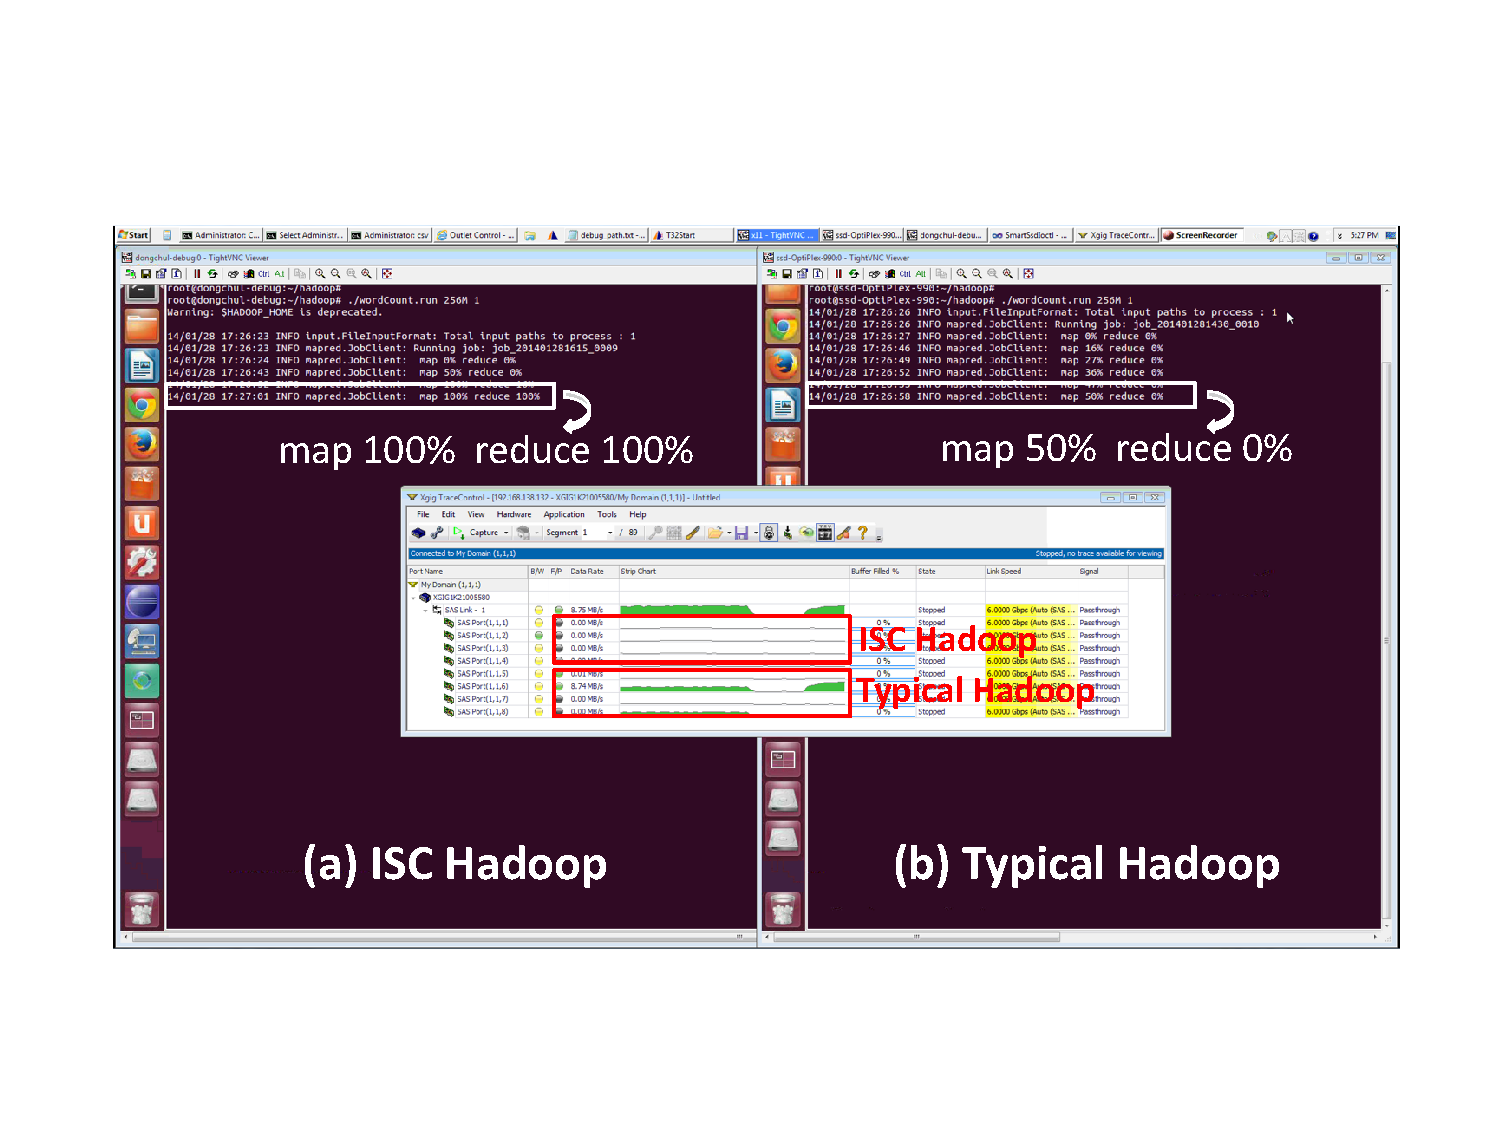
\includegraphics[width=1.0\columnwidth]{figures/ISC_Hadoop_demo.pdf}
	\caption{Hadoop System Demonstration (ISC Hadoop vs. Typical Hadoop)}
	\label{fig:ISC_Hadoop_demo}
\end{figure}







\begin{figure*}[t]
  \centering
  \renewcommand{\tabcolsep}{0.1mm}
  \begin{tabular}{ccc}
 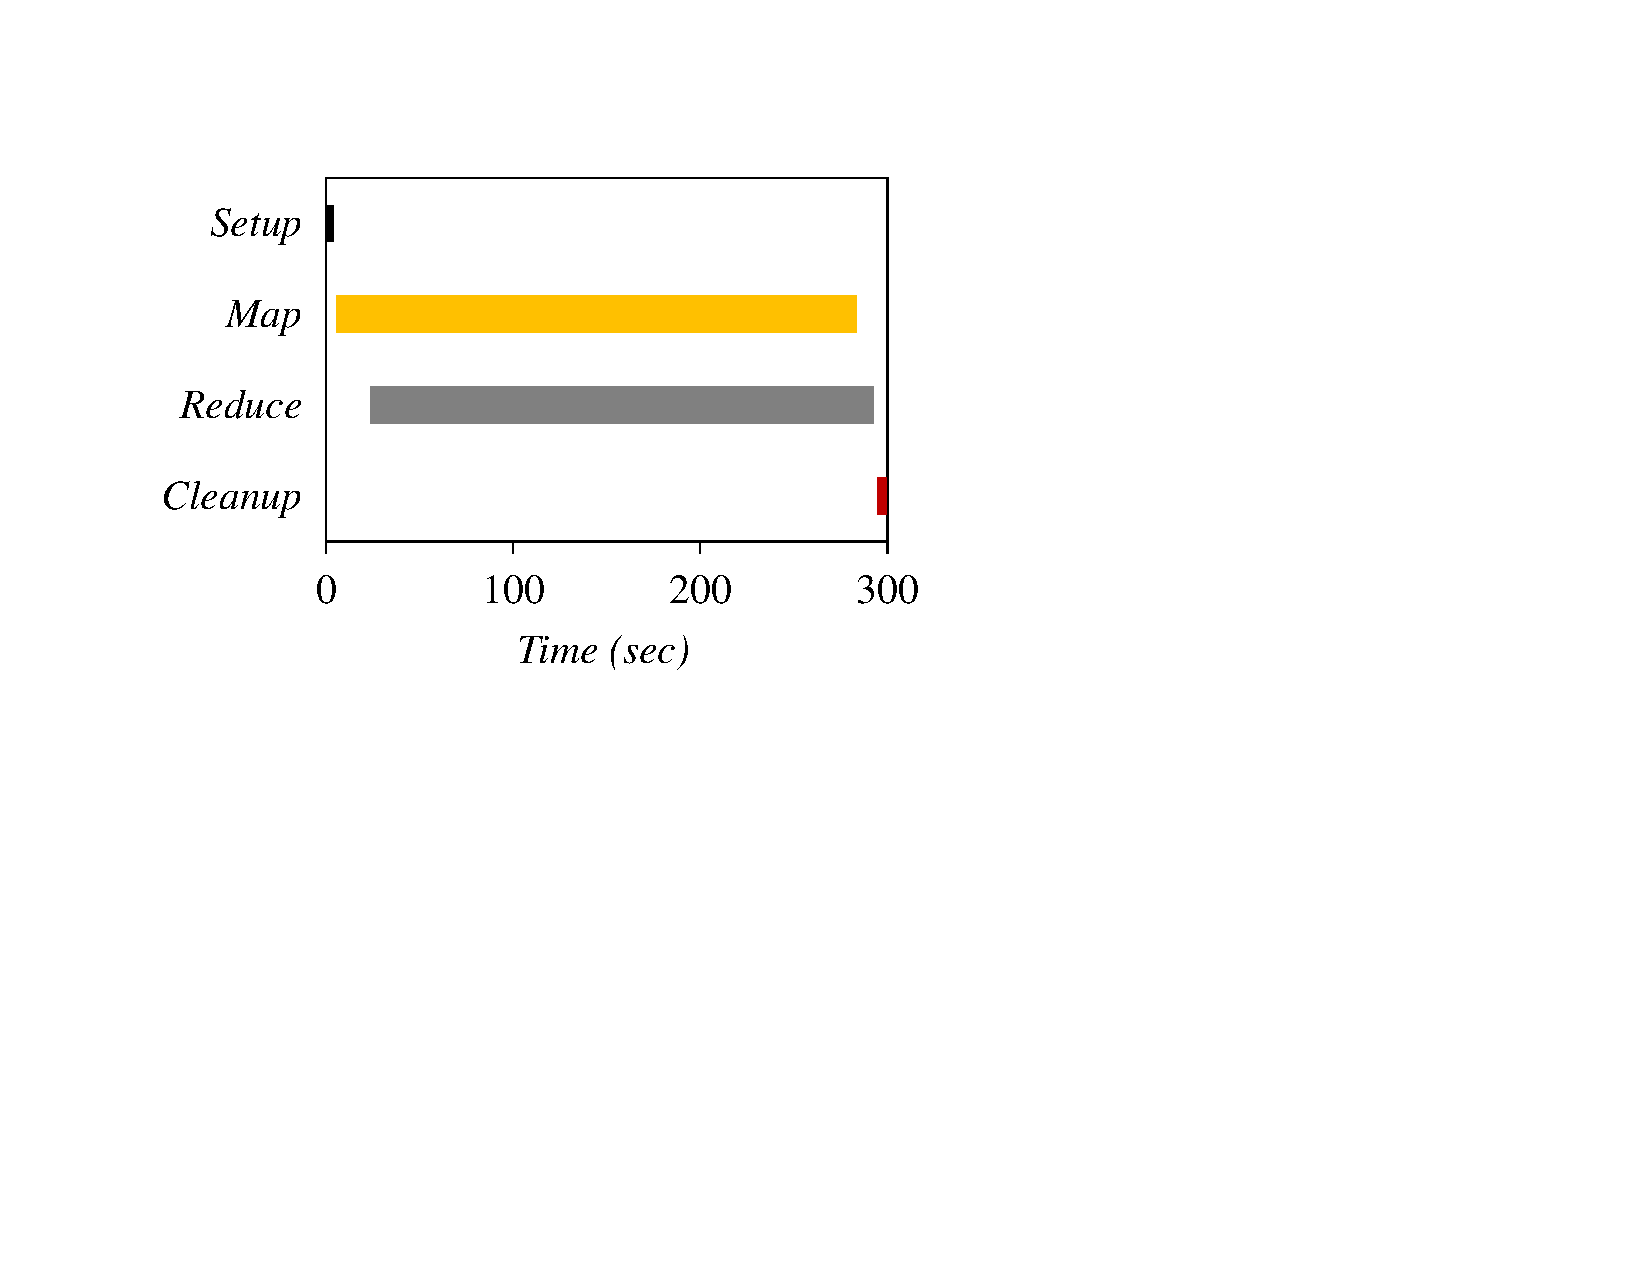
\includegraphics[width=0.69\columnwidth]{figures/Hadoop_execution_time_each_phase_breakdown2.pdf}&
  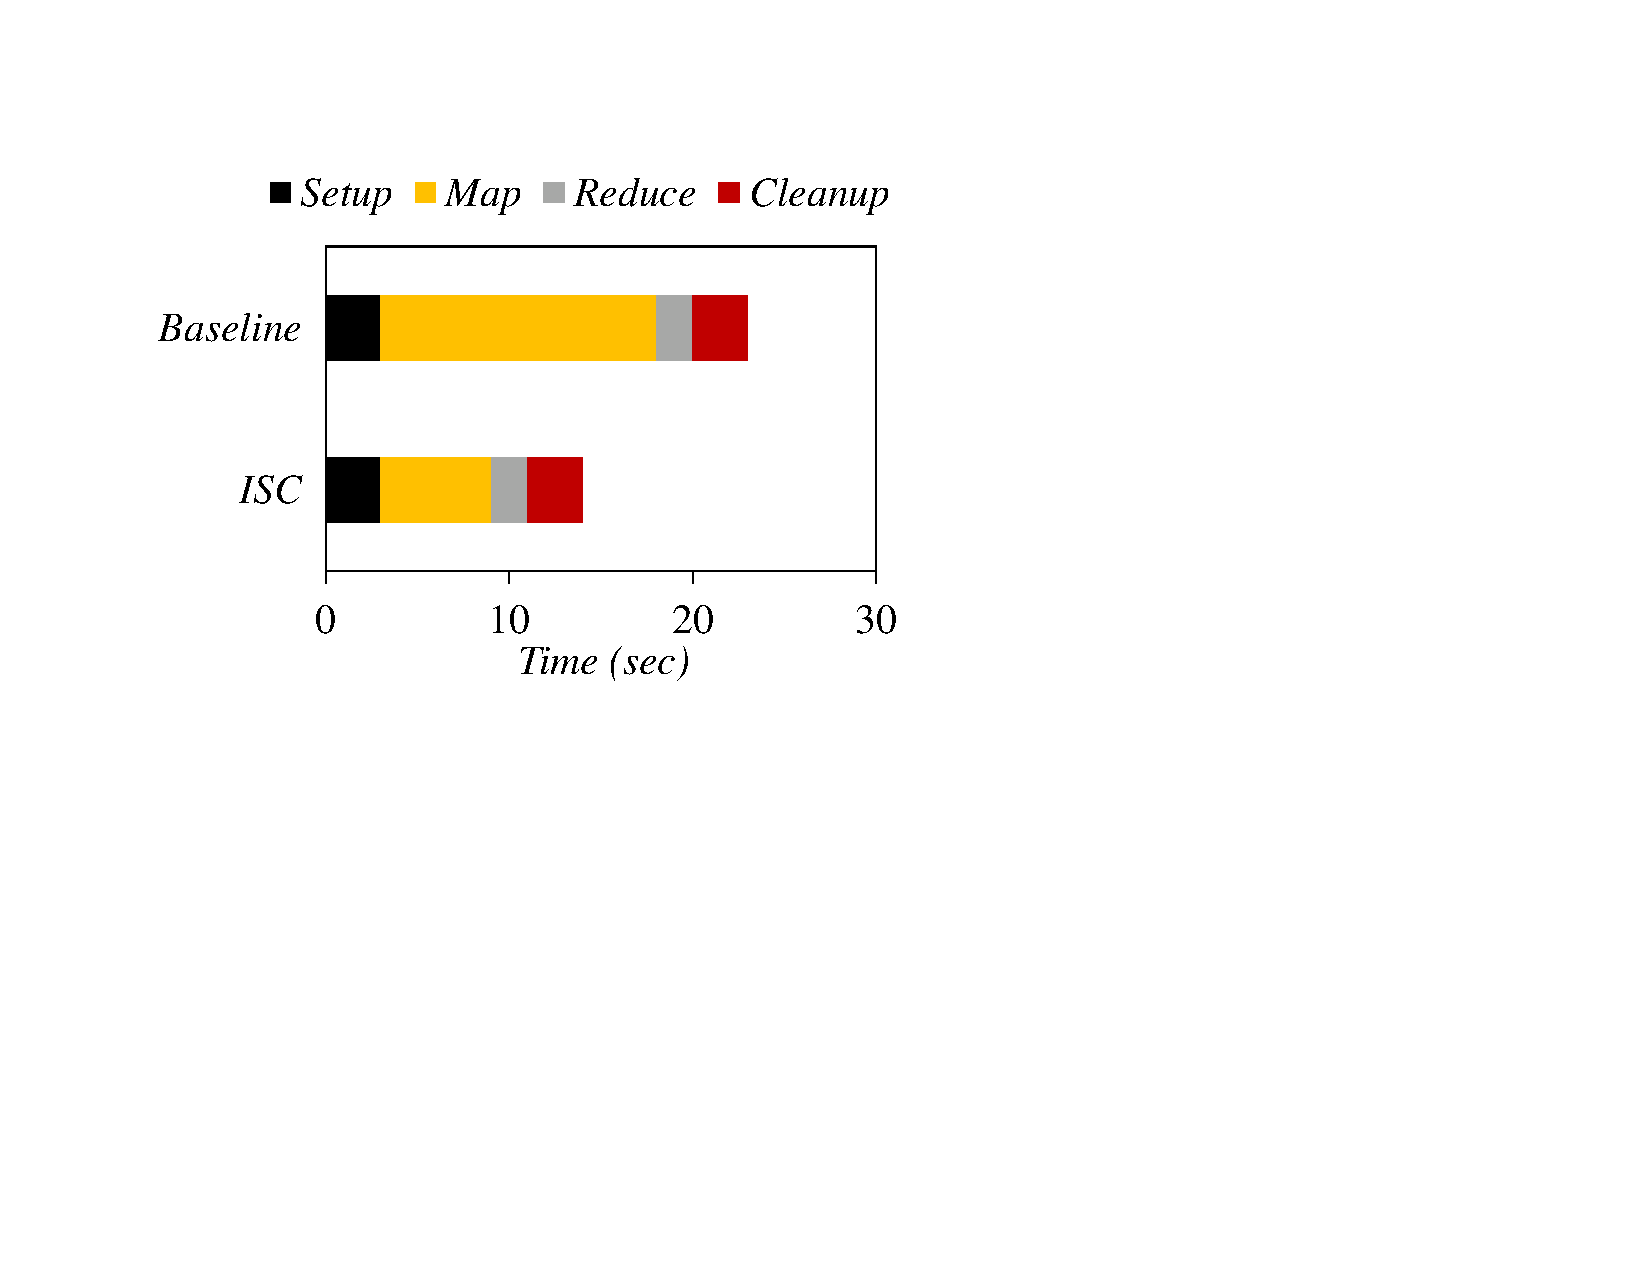
\includegraphics[width=0.69\columnwidth]{figures/Hadoop_time_breakdown1.pdf}&
  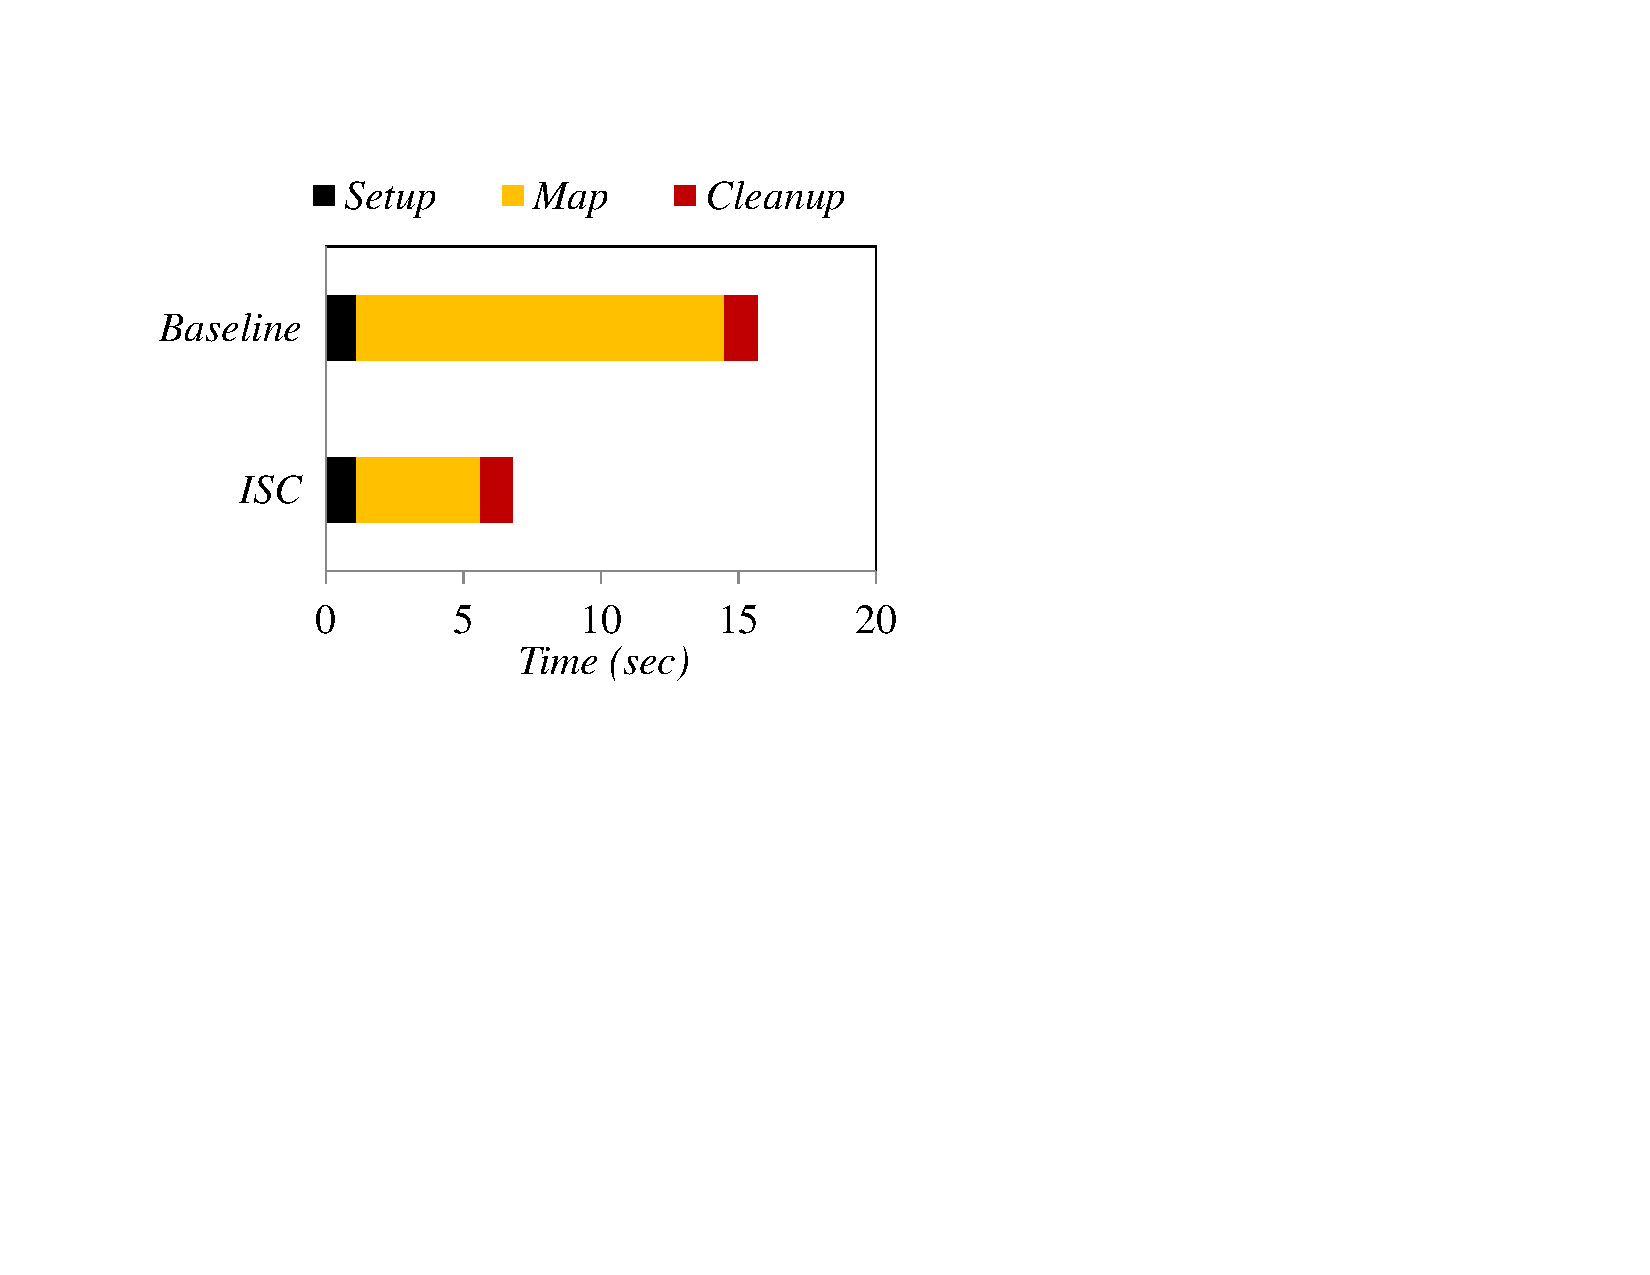
\includegraphics[width=0.69\columnwidth]{figures/Hadoop_breakdown_per_maptask1.pdf}\\	
  (a) Per Job & (b) Per Task & (c) Per Map Task
\end{tabular}
  \caption{Breakdown of each Hadoop execution time}
  \label{fig:time_breakdown}
 \end{figure*}




\subsubsection{A Single Node}\label{subsubsec:Exp_result_singlenode}
We set up two Hadoop systems for the fully distributed mode on a single node: (1) a single instance of both namenode and datanode (this corresponds to a pseudo distributed mode) and (2) a single instance of namenode and two instances of datanode. 








\begin{figure}[t]
  \centering
  \renewcommand{\tabcolsep}{0.1mm}
  \begin{tabular}{ccc}
 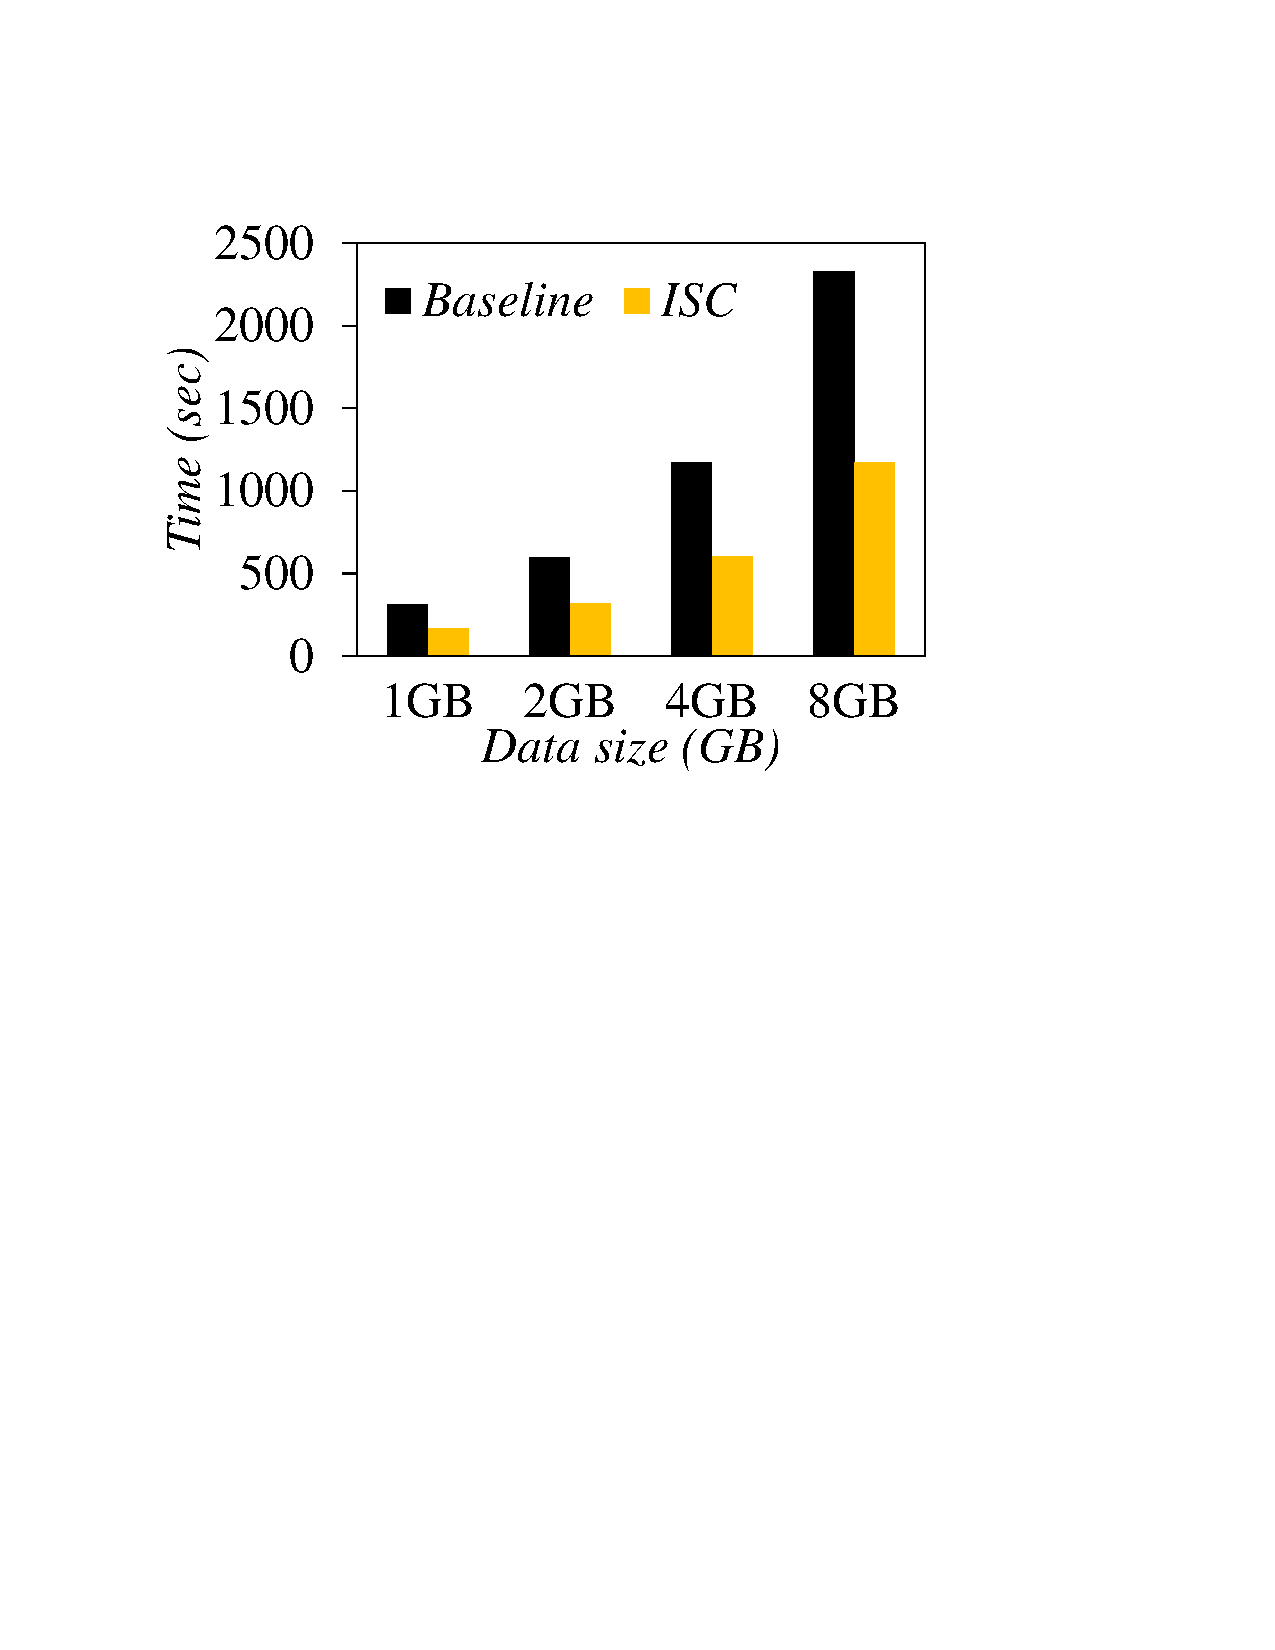
\includegraphics[width=0.5\columnwidth]{figures/Singlenode_Total_Elapsed_Time.pdf}&
  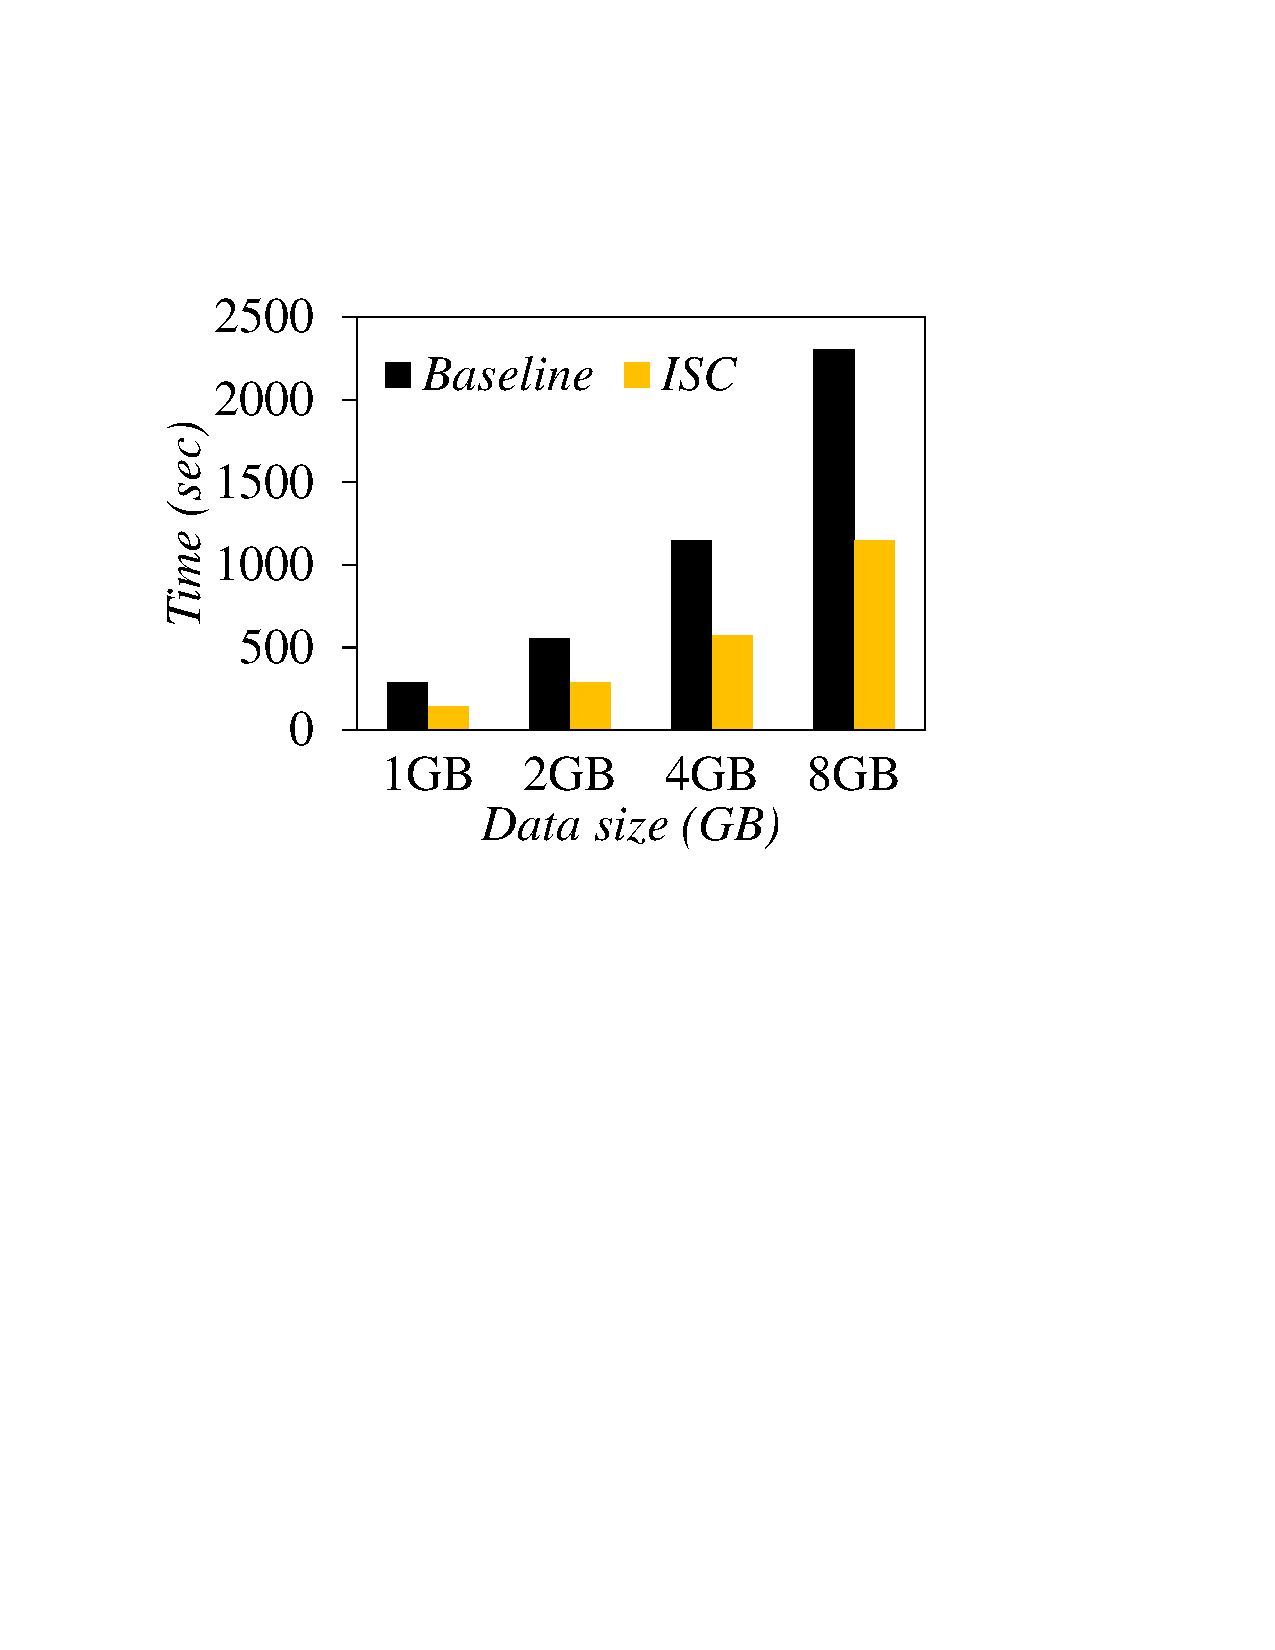
\includegraphics[width=0.5\columnwidth]{figures/Singlenode_Total_Mapper_Elapsed_Time.pdf}\\
  (a) Total Elapsed Time & (b) Total Mapper Elapsed Time
\end{tabular}
  \caption{Total elapsed time on a single node (single datanode and single namenode)}
  \label{fig:execution_time_with_single_namenode_on_single_node}
 \end{figure}






\textbf{Total elapsed time:} Figure~\ref{fig:execution_time_with_single_namenode_on_single_node} shows a total elapsed time on a single node with a single namenode and datanode. Our ISC Hadoop system achieves 2$\times$ faster than the typical Hadoop system in terms of a total elapsed time (i.e. end-to-end total execution time) (please refer to Figure~\ref{fig:execution_time_with_single_namenode_on_single_node} (a)). Figure~\ref{fig:execution_time_with_single_namenode_on_single_node} (b) displays a total elapsed time in a Mapper phase by excluding all other phases. This shows how much time each Hadoop system consumes to complete all Map tasks. Similarly, our ISC Hadoop system completes all Map tasks 2$\times$ faster than the baseline system. The results and trends in Figure~\ref{fig:execution_time_with_single_namenode_on_single_node} (b) are almost identical to those in Figure~\ref{fig:execution_time_with_single_namenode_on_single_node} (a). This is because the total execution time of all Map tasks is a significantly dominant factor of the total Hadoop running time in wordcount-like Hadoop applications (for instance, 91\% with 1GB data -- 98\% with 8GB data of the total wordcount execution time).
Figure~\ref{fig:time_breakdown} (a) demonstrates well this analysis. It breaks down the total execution time of wordcount into each Hadoop phase (baseline with 1GB data on a single node). After a short Hadoop setup time (3 seconds), the Hadoop system keeps executing each Map task (277 seconds) and completed Map tasks trigger executing a corresponding Reduce task with their output data in parallel. The total execution time of Reduce tasks (268 seconds) almost overlaps with that of Map task since it is heavily dependent on Map task completion. Lastly, Hadoop cleanup time takes about 3 seconds. 




%\begin{figure}[htbp]
%	\centering
%		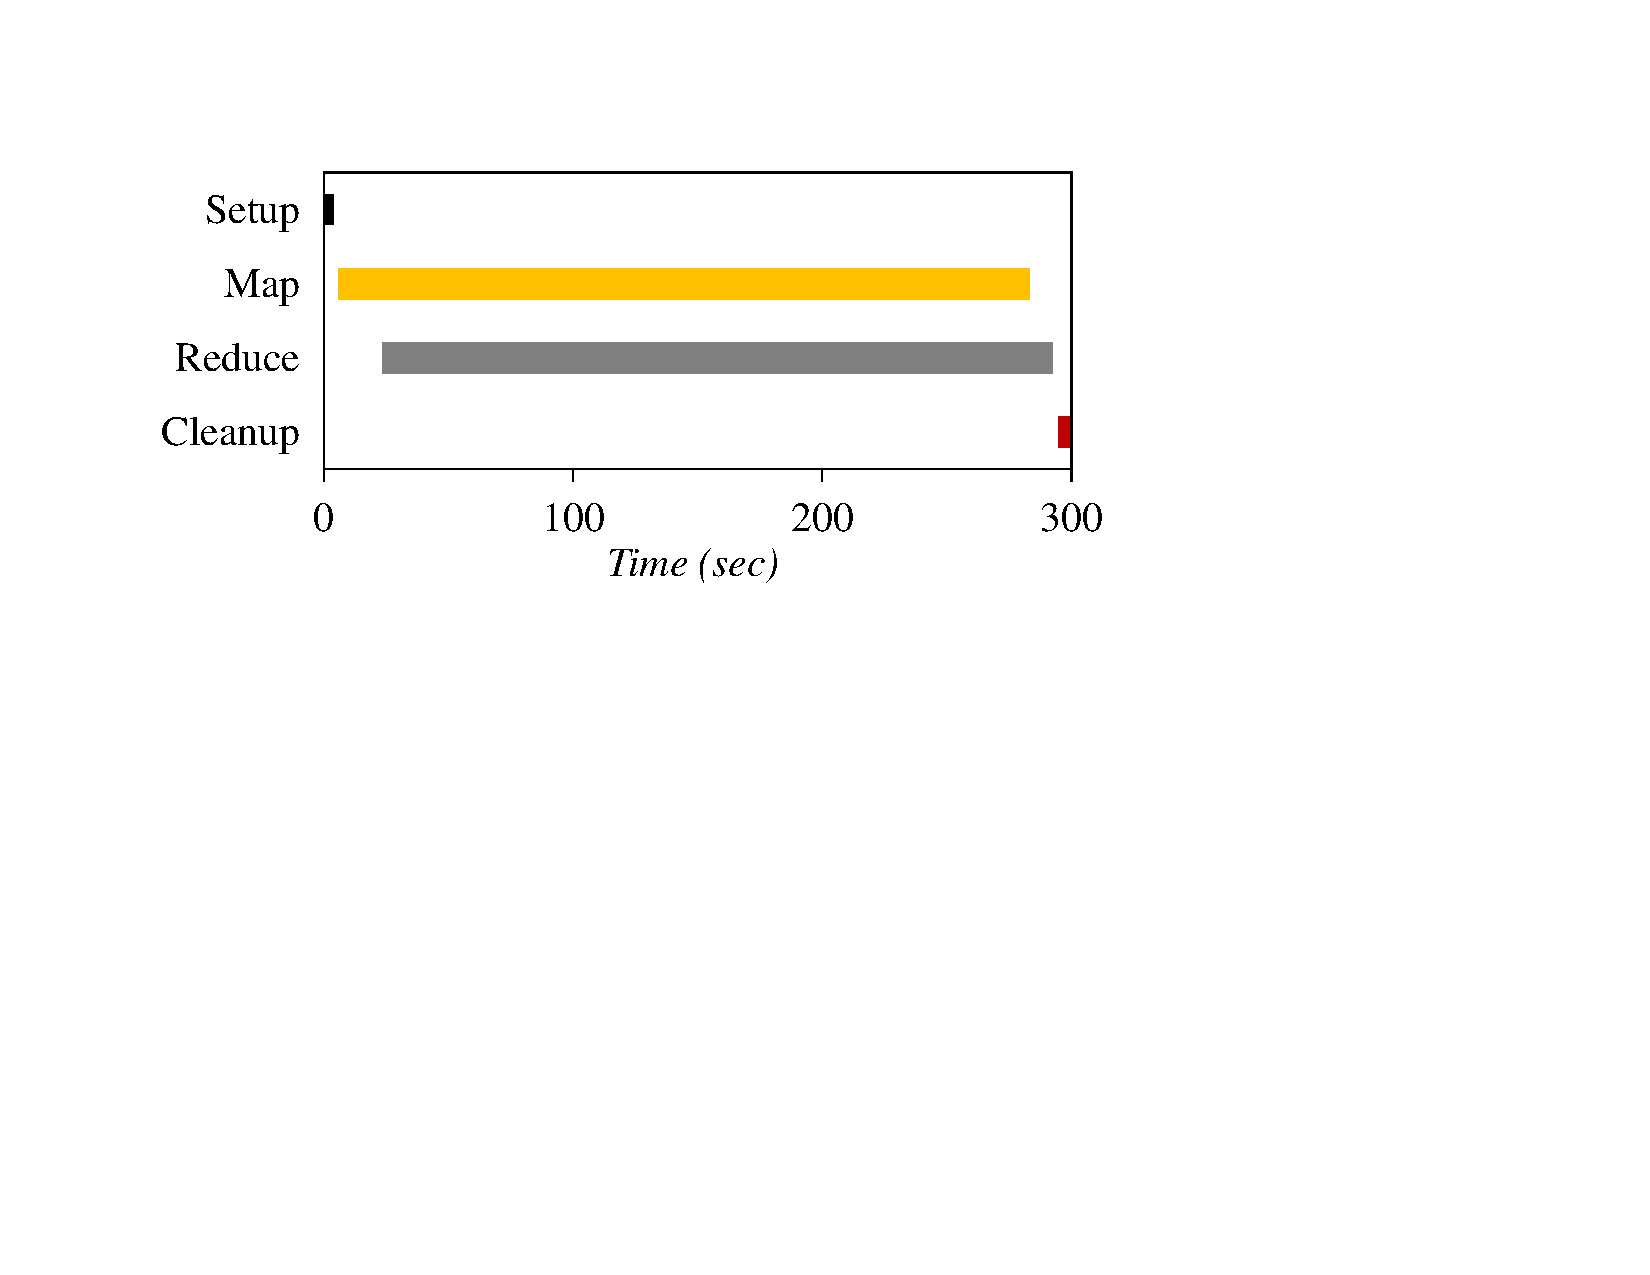
\includegraphics[width=0.8\columnwidth]{figures/Hadoop_execution_time_each_phase_breakdown1.pdf}
%	\caption{Total elapsed time breakdown of each phase}
%	\label{fig:Hadoop_total_time_BreakDown}
%\end{figure}


Figure~\ref{fig:time_breakdown} (b) makes a deeper analysis of the Hadoop task execution time. This figure shows the elapsed time of each Hadoop phase per each task. Each Hadoop task is subdivided into Map task and Reduce task. As a matter of fact, Hadoop sets up a job (setup time) at the beginning and deletes all intermediate data (cleanup time) after the job completion. These two tasks are performed only one time respectively throughout the whole job execution. That is, the total execution time of Hadoop application can be largely composed of one-time job setup time, many (depending on a data size) Map and Reduce tasks execution time, and one-time cleanup time. Considering this fact, Mapper execution time is a dominant factor of a total Hadoop execution time in wordcount-like Hadoop application. Based on these observations, our proposed ISC Hadoop framework moves Mapper to our ISC devices to improve Hadoop performance. As shown in Figure~\ref{fig:time_breakdown} (b), our ISC Hadoop system improves the Map task execution time by 2.5$\times$ faster (from 15 seconds to 6 seconds). All of our performance gain stems from this Mapper improvement.  


%\begin{figure}[htbp]
%	\centering
%		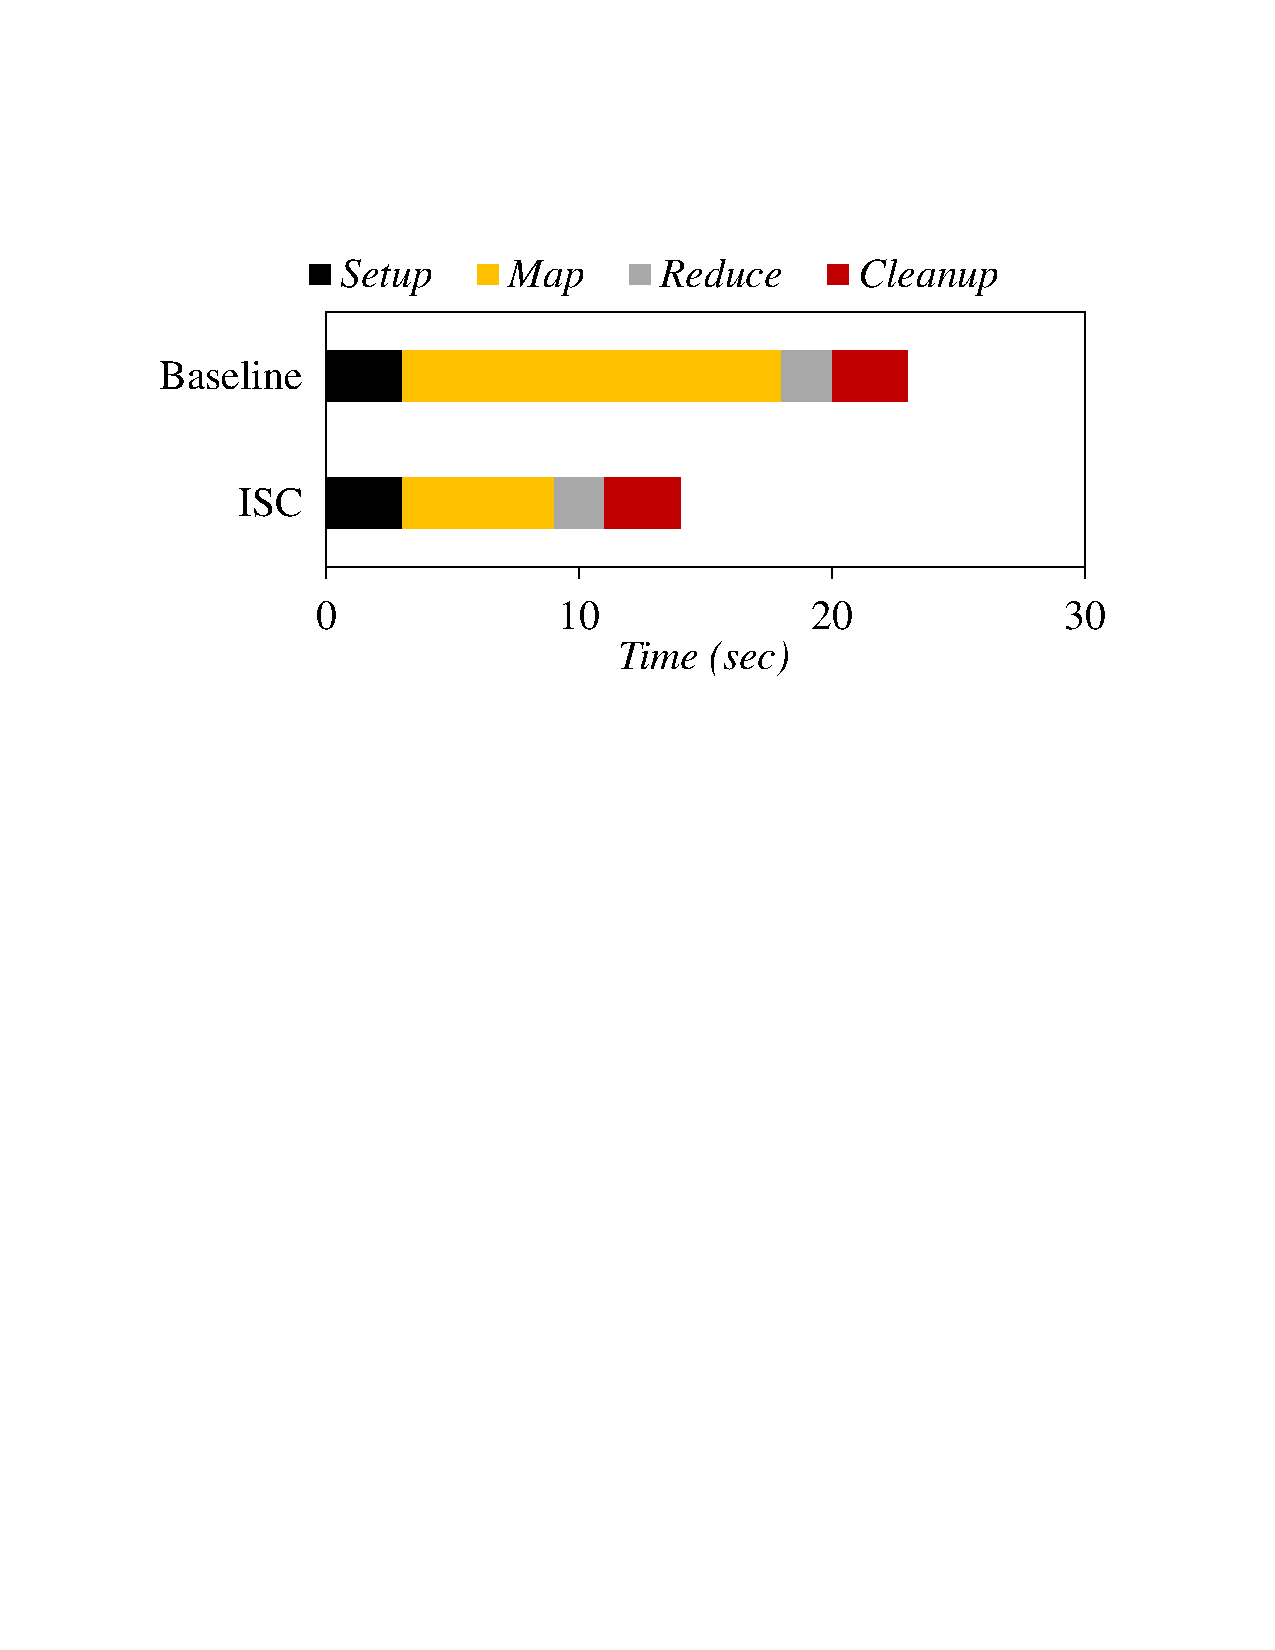
\includegraphics[width=0.8\columnwidth]{figures/Hadoop_time_breakdown.pdf}
%	\caption{Elapsed time breakdown per Hadoop task. Note: both setup and cleanup time here are one-time task per job, not per task.}
%	\label{fig:Hadoop_timeBreakDown}
%\end{figure}



Figure~\ref{fig:time_breakdown} (c) provides a even deeper analysis of the Mapper execution time. This plot corresponds to Map task execution time (i.e., yellow bar) in the Figure~\ref{fig:time_breakdown} (b). Similarly, Map task execution time is subdivided further into three elements: Map task setup time, Map task execution time, and Map task cleanup time. Both Map task setup time and cleanup time are almost constant time (in total 1.2 seconds). Thus, if we compare a \emph{pure} Map task execution time (i.e., yellow bar in the Figure~\ref{fig:time_breakdown}) (c) between them, our performance gain is even larger (3.6$\times$). However, each Map task requires such extra constant time (i.e., both Map task setup time and cleaning time, about 2--3 sec/Map) as well as Map task execution time. This constant time is relatively big portion (about 36\%) to Map task in ISC Hadoop system, compared to the portion (14.6\%) in baseline. Therefore, this larger performance gain (3.6$\times$) is lessened to 2.5$\times$ in Figure~\ref{fig:time_breakdown} (b), and similarly to 2$\times$ in end-to-end total execution time (Figure~\ref{fig:execution_time_with_single_namenode_on_single_node}).


%\begin{figure}[htbp]
%	\centering
%		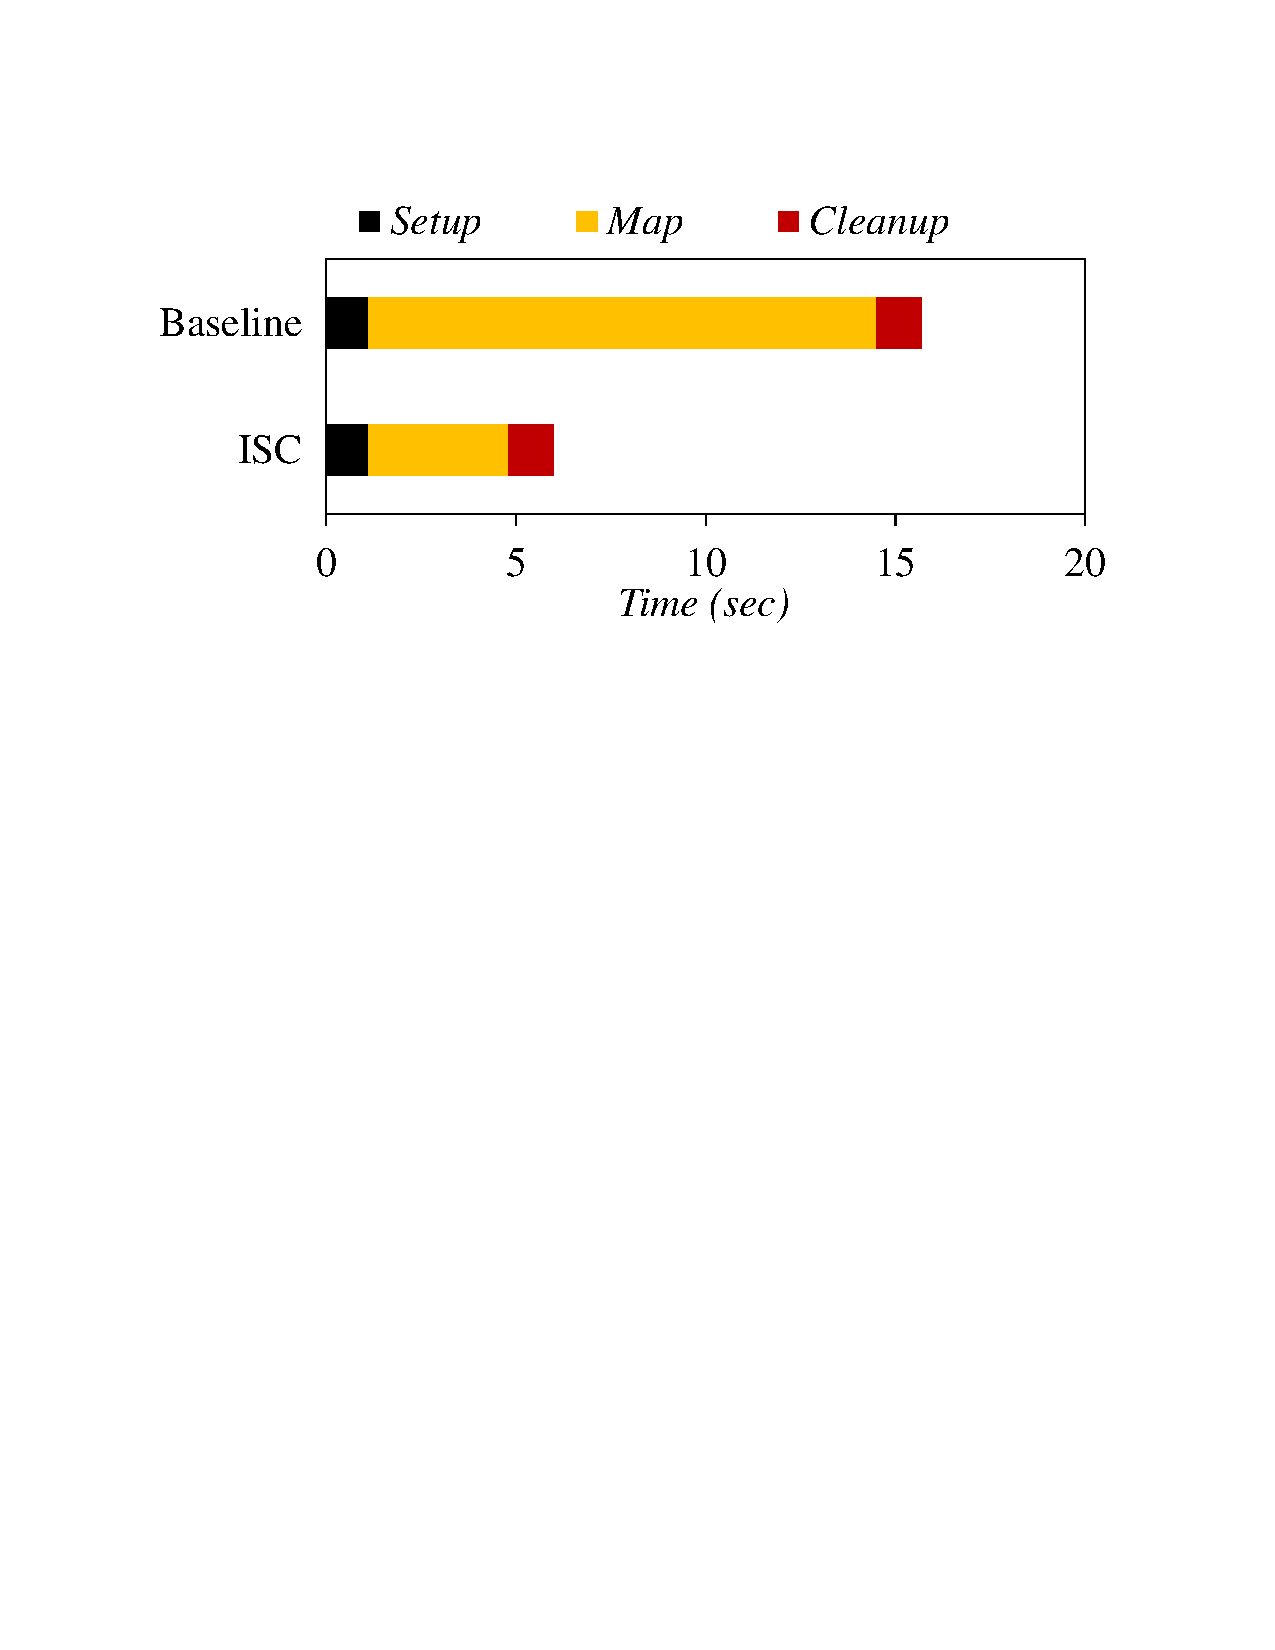
\includegraphics[width=0.8\columnwidth]{figures/Hadoop_breakdown_per_maptask.pdf}
%	\caption{Elapsed time breakdown per Map task}
%	\label{fig:Hadoop_timeBreakDown_per_mapTask}
%\end{figure}



\begin{figure}[htbp]
  \centering
  \renewcommand{\tabcolsep}{0.1mm}
  \begin{tabular}{ccc}
 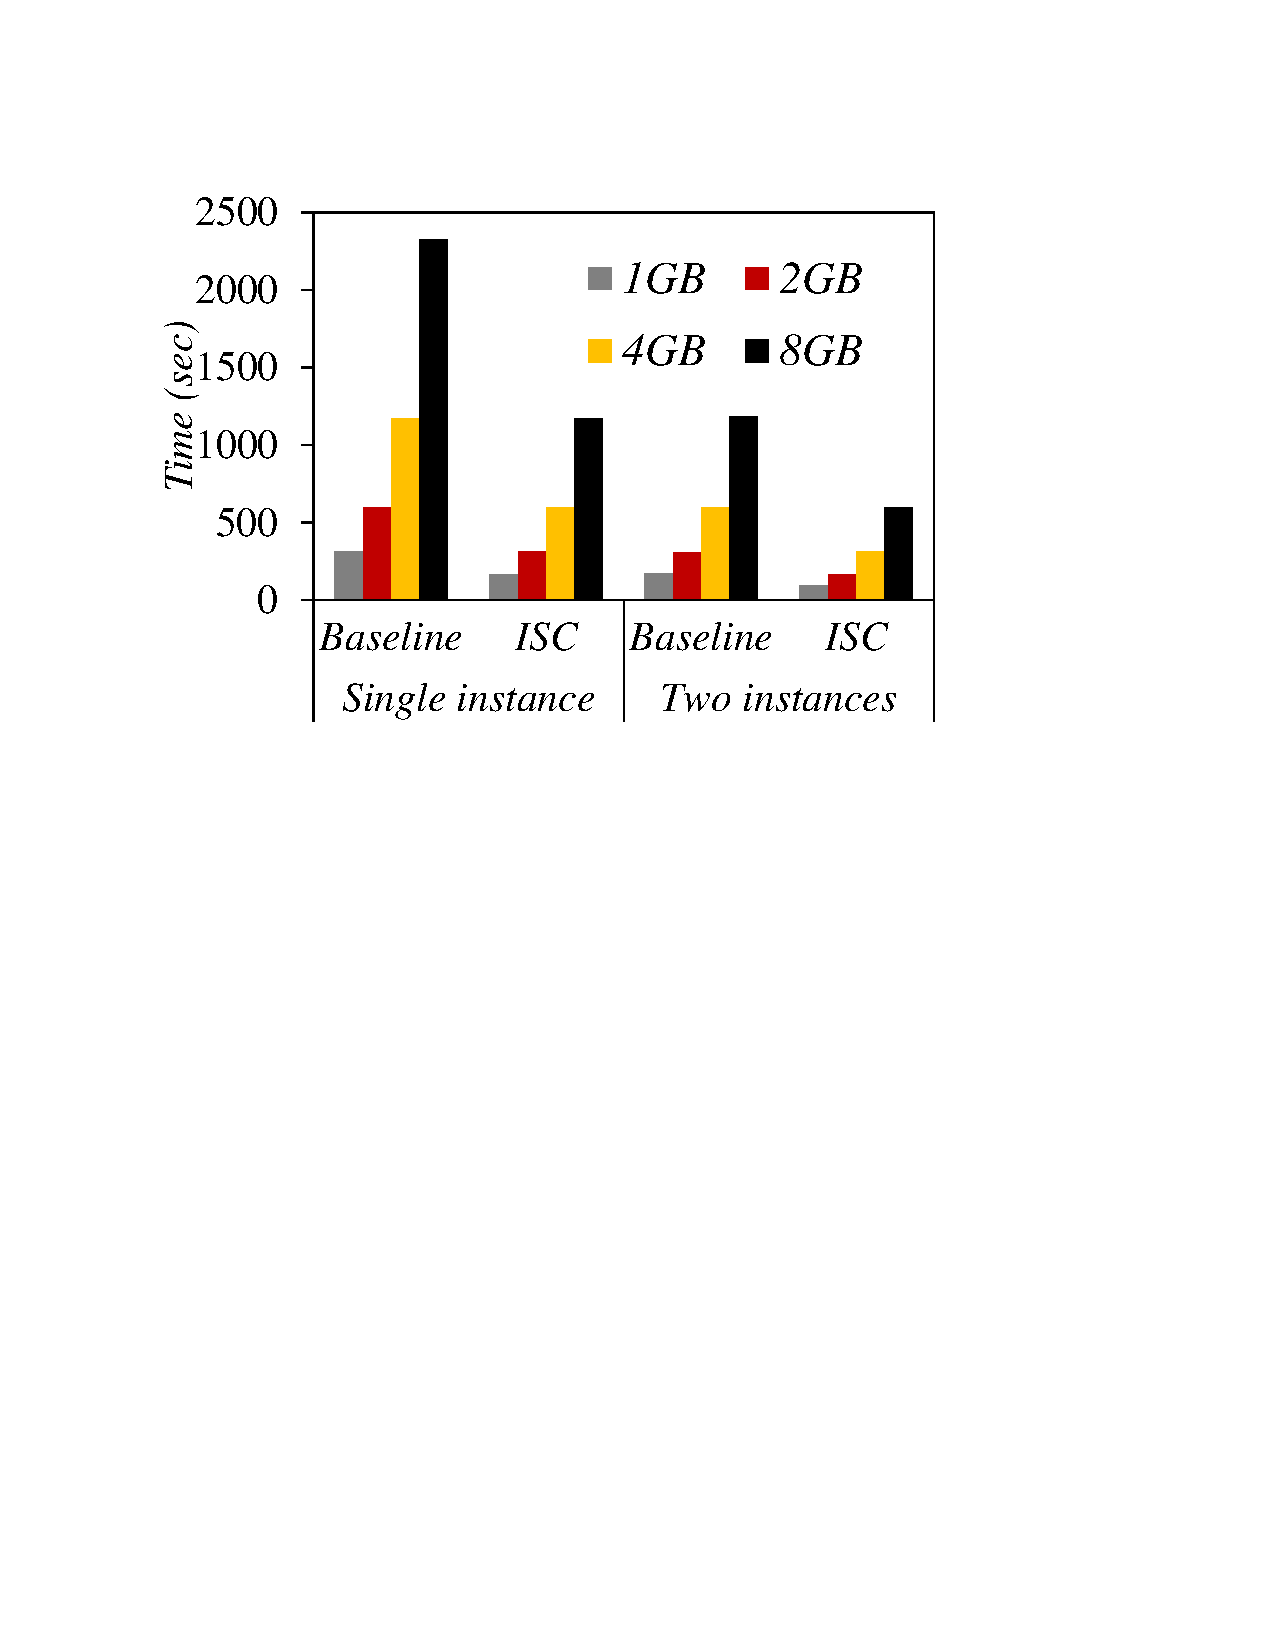
\includegraphics[width=0.5\columnwidth]{figures/Hadoop_total_execution_time_single_two_nodes.pdf}&
  %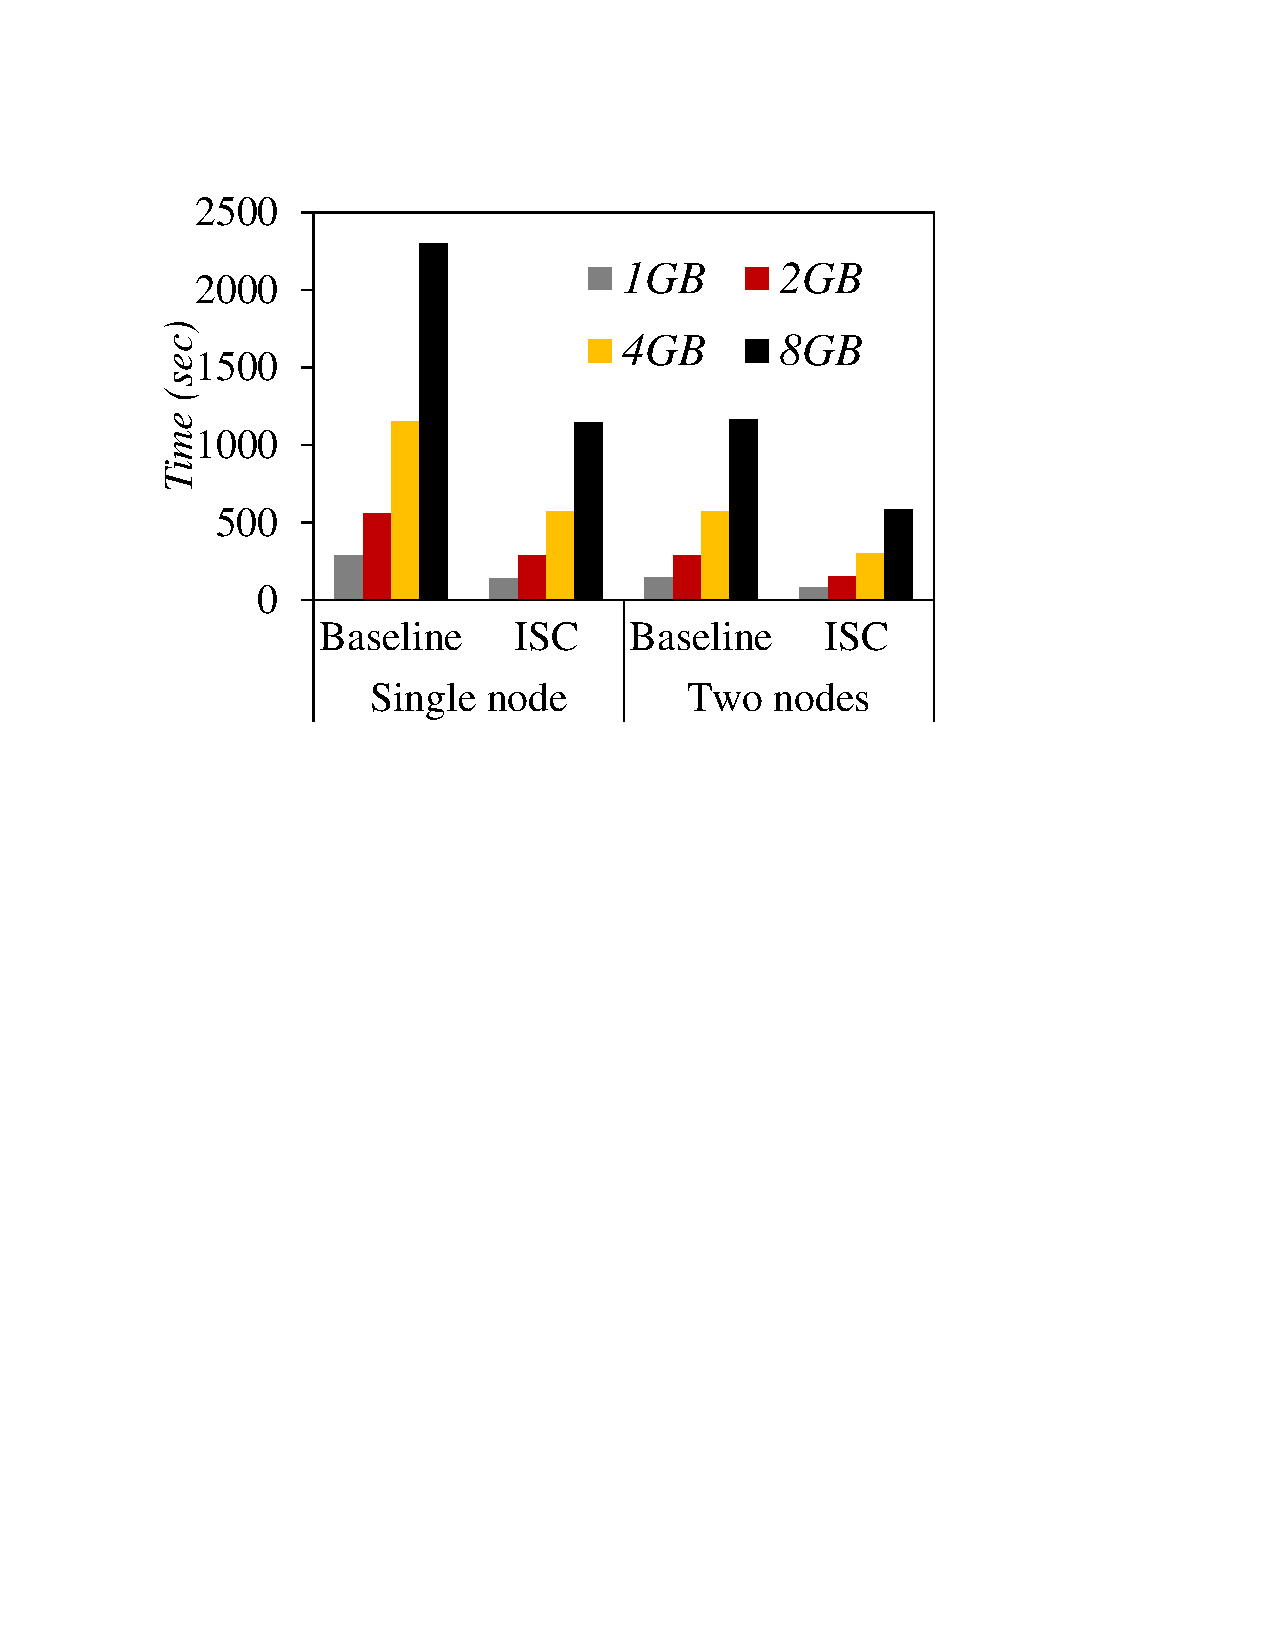
\includegraphics[width=0.5\columnwidth]{figures/Hadoop_mapper_execution_time_single_two_nodes.pdf}\\
  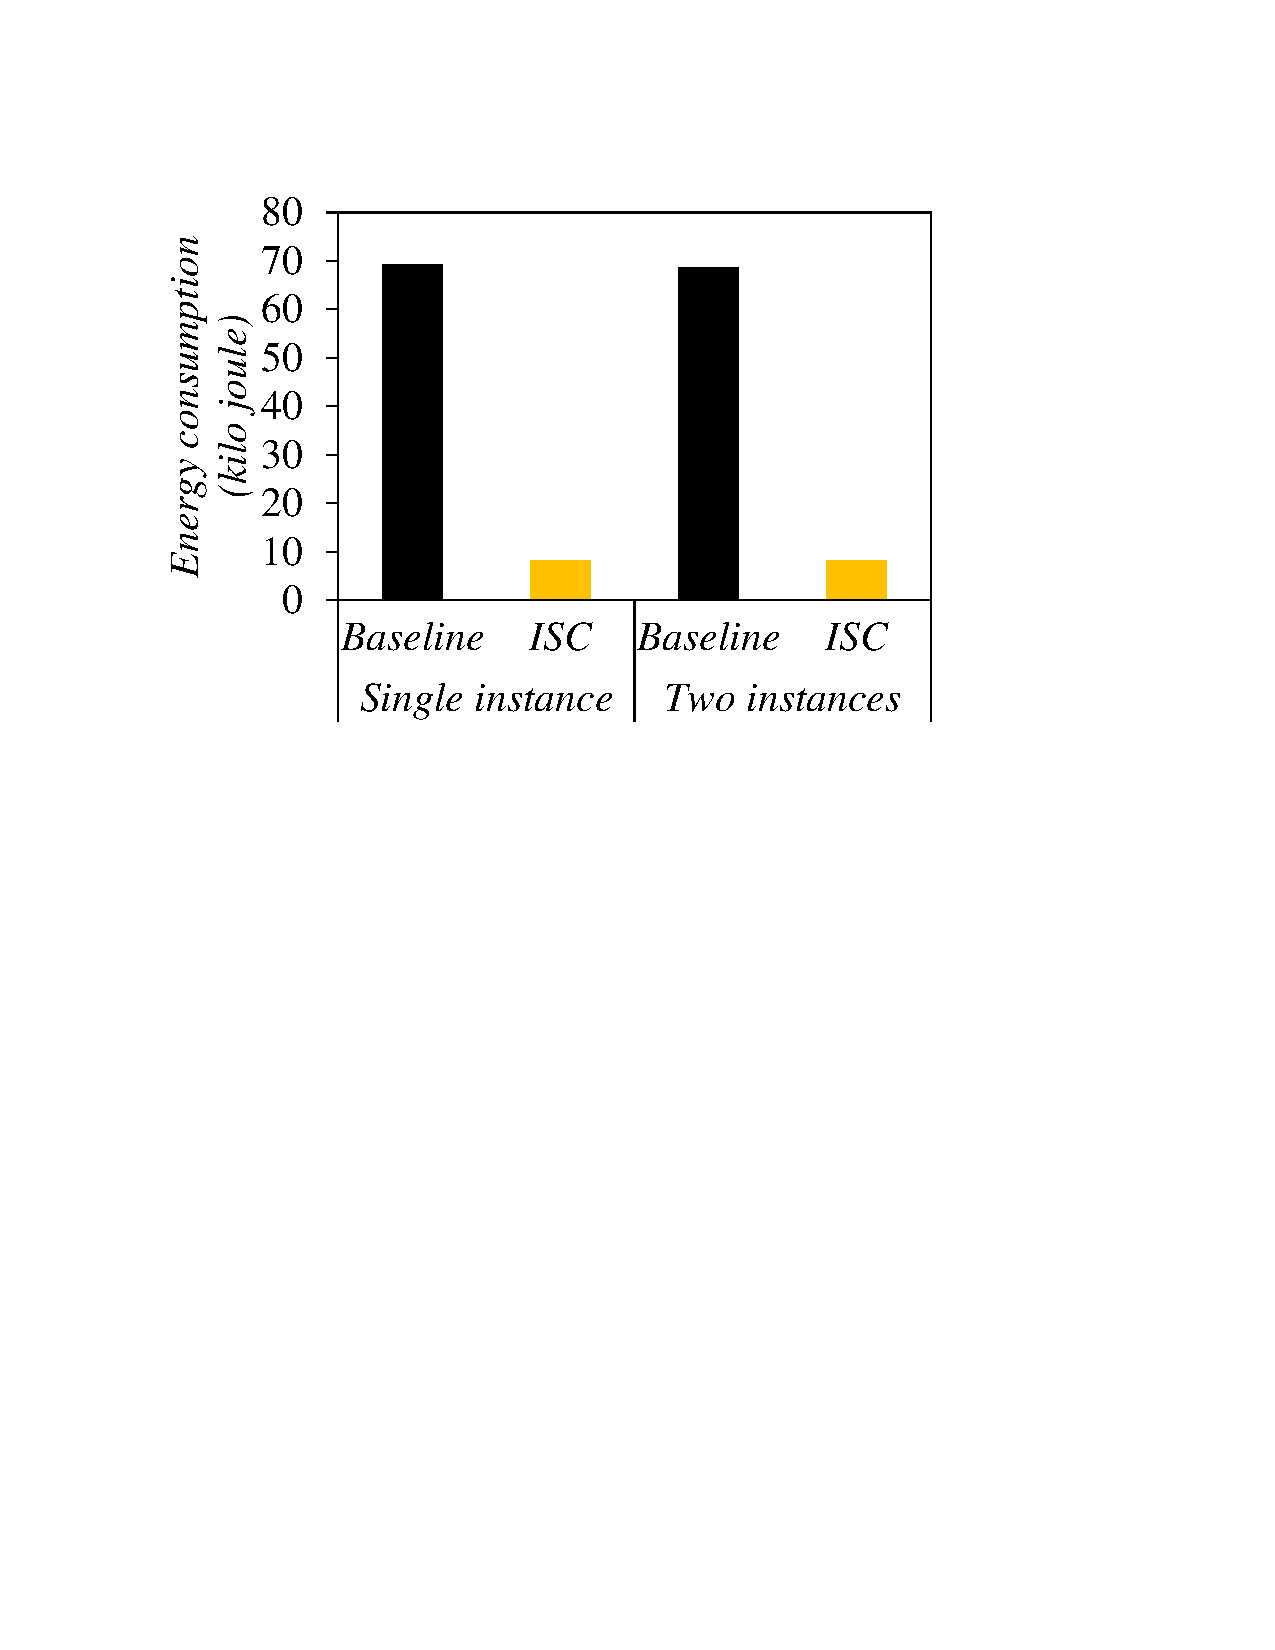
\includegraphics[width=0.5\columnwidth]{figures/Hadoop_power_consumption_single_node.pdf}\\	
  (a) Total Elapsed Time & (b) Total Energy Consumption
\end{tabular}
  \caption{Single instance vs. two instances on a single node}
  \label{fig:execution_time_with_two_namenode_on_single_node}
 \end{figure}




\begin{figure*}[t]
  \centering
  \renewcommand{\tabcolsep}{1mm}
  \begin{tabular}{ccc}
 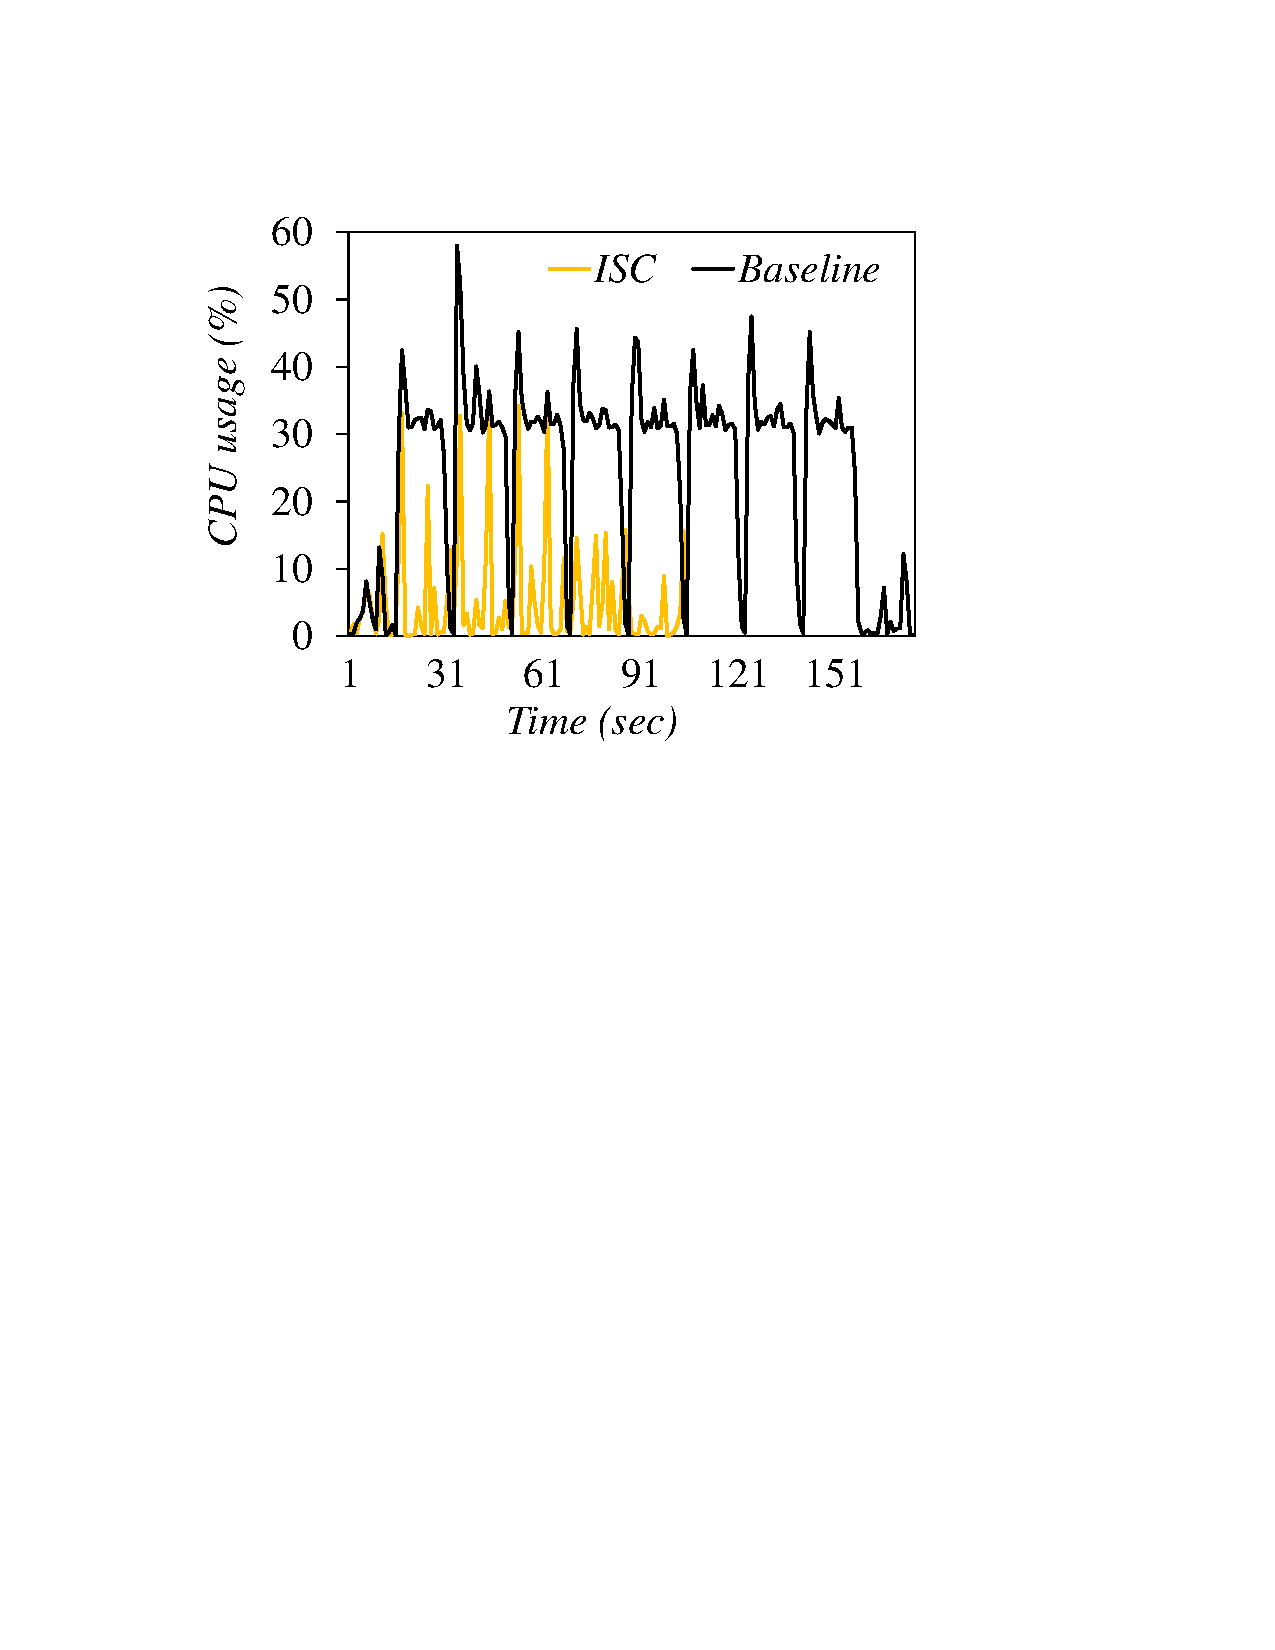
\includegraphics[width=0.66\columnwidth]{figures/Hadoop_CPU_usage.pdf}&
  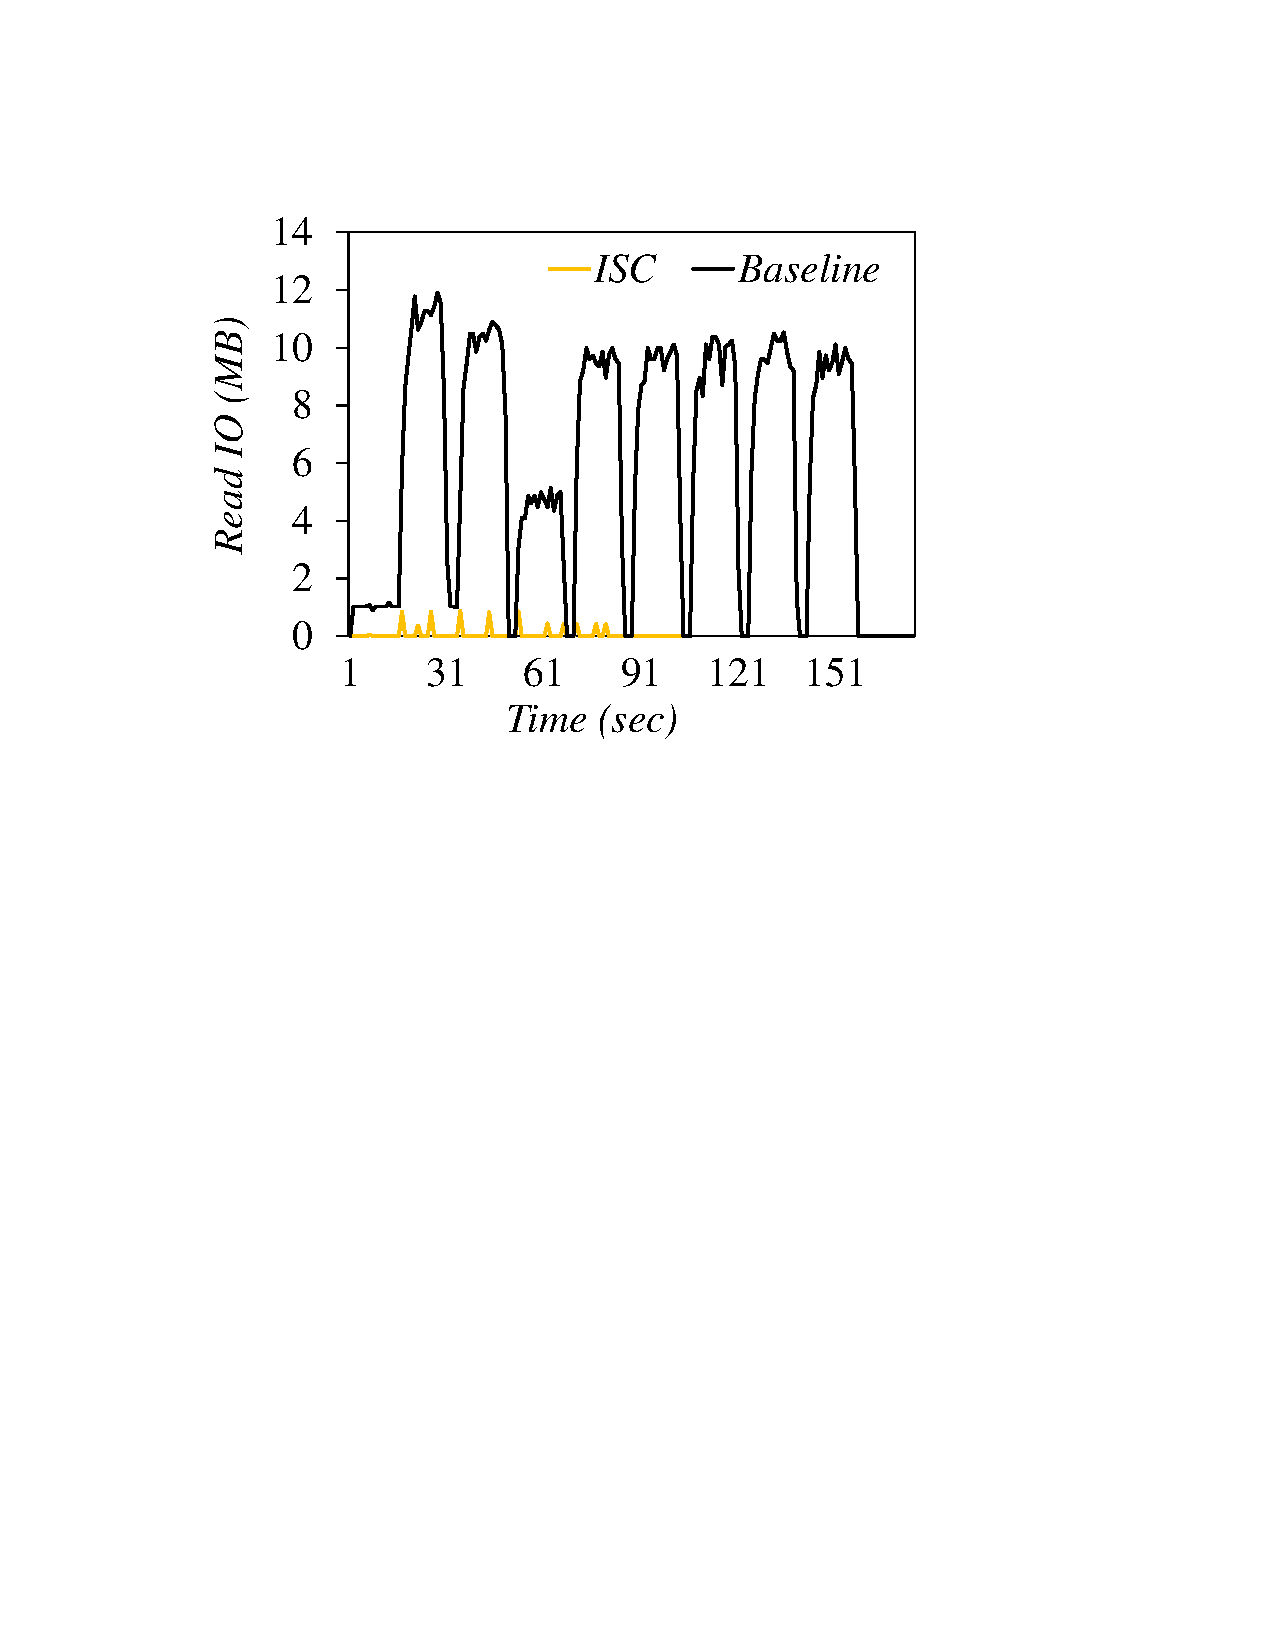
\includegraphics[width=0.66\columnwidth]{figures/Hadoop_read_io.pdf}&
  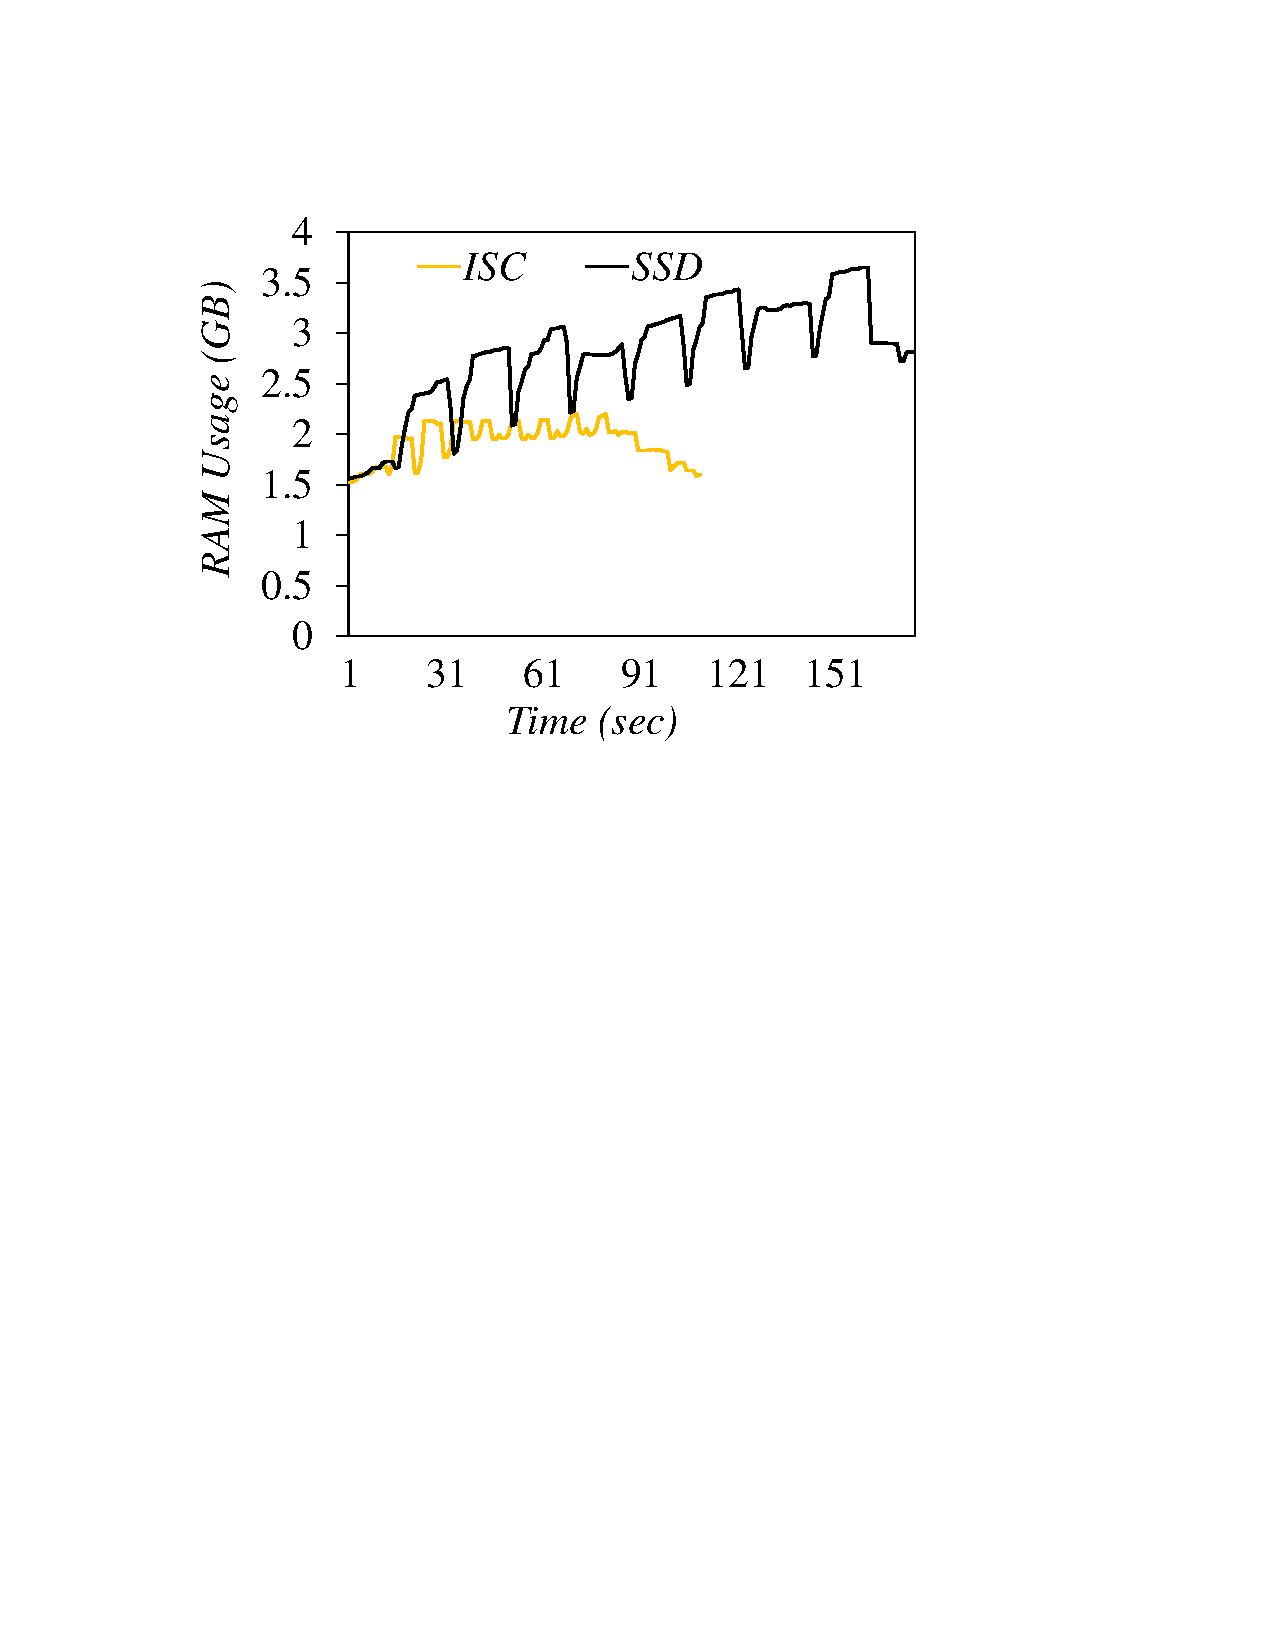
\includegraphics[width=0.66\columnwidth]{figures/Hadoop_RAM_usage.pdf}\\	
  (a) Host CPU Usage & (b) Host Read I/O & (c) Host DRAM Usage
\end{tabular}
  \caption{Host system resource usage}
  \label{fig:host_resource_usage}
\end{figure*}


\begin{figure*}[t]
  \centering
  \renewcommand{\tabcolsep}{1mm}
  \begin{tabular}{ccc}
 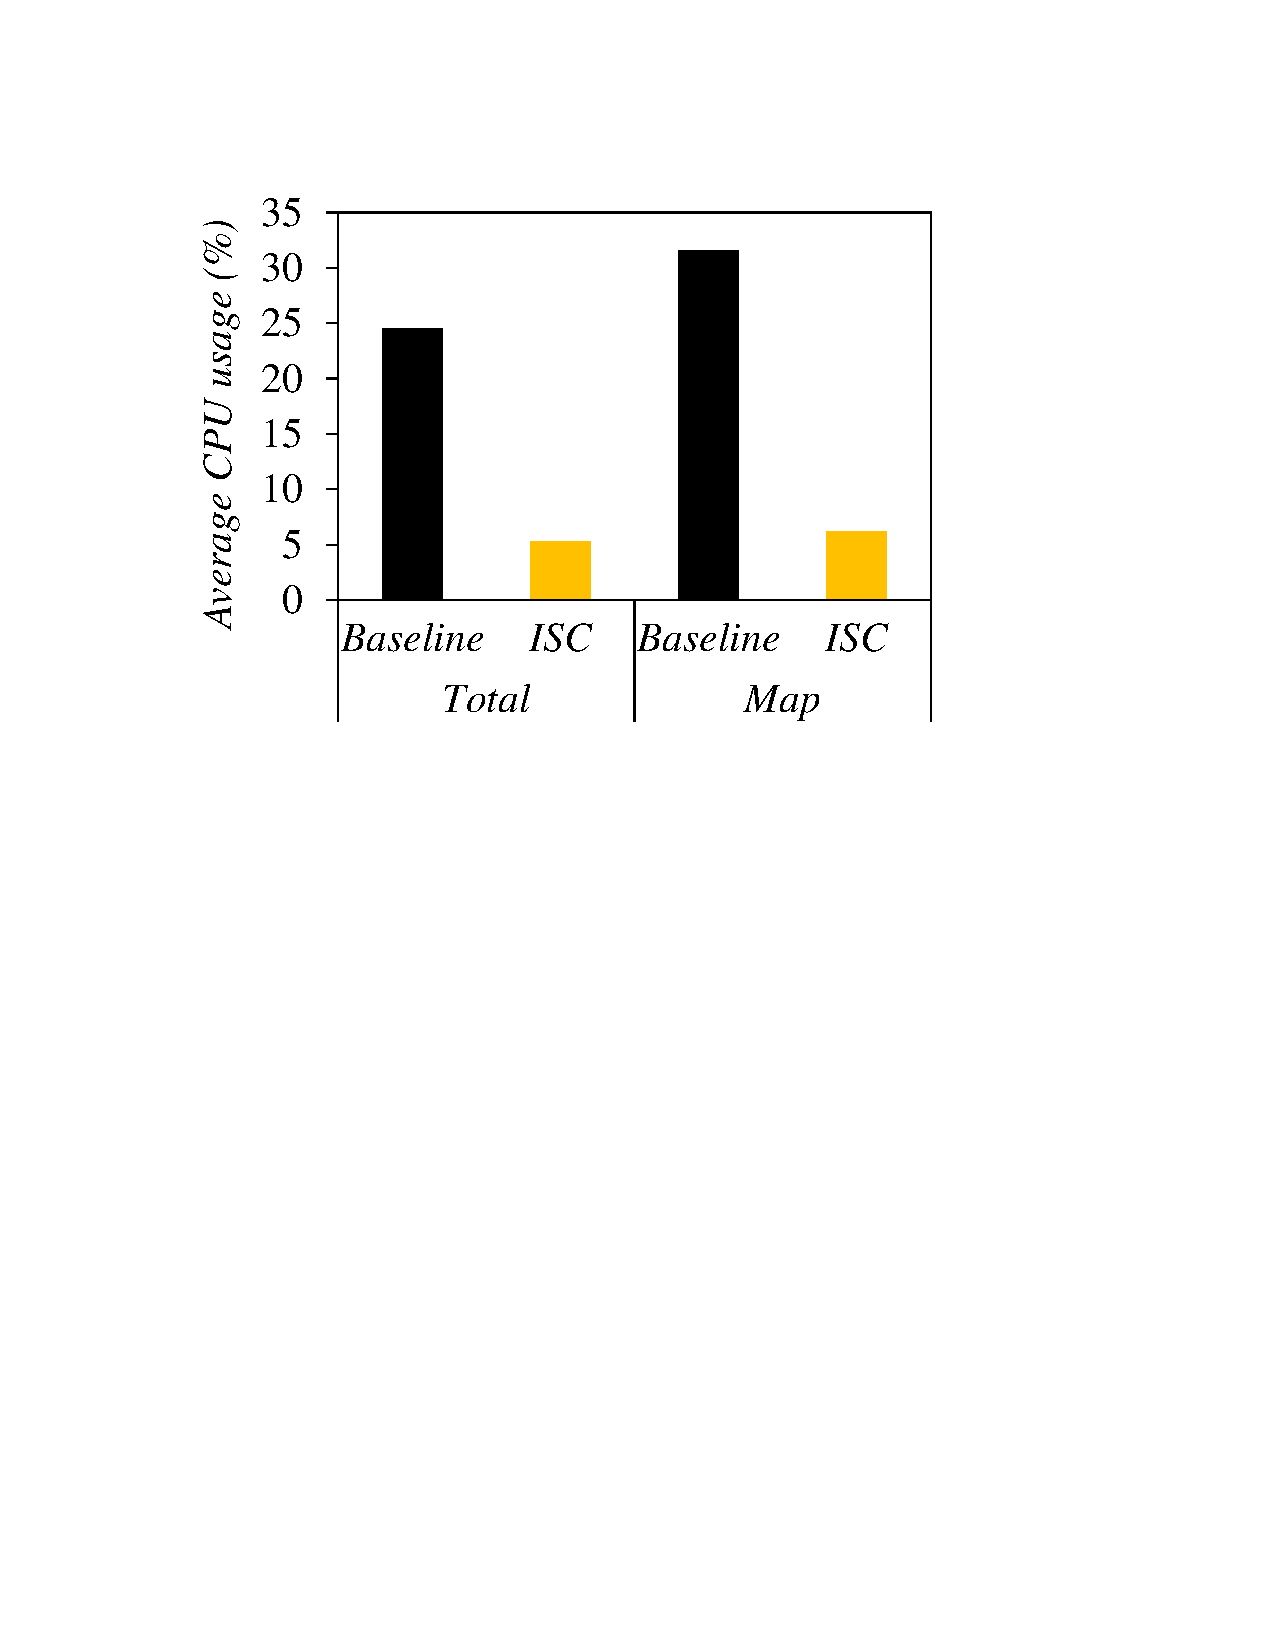
\includegraphics[width=0.66\columnwidth]{figures/Hadoop_average_CPU_usage.pdf}&
  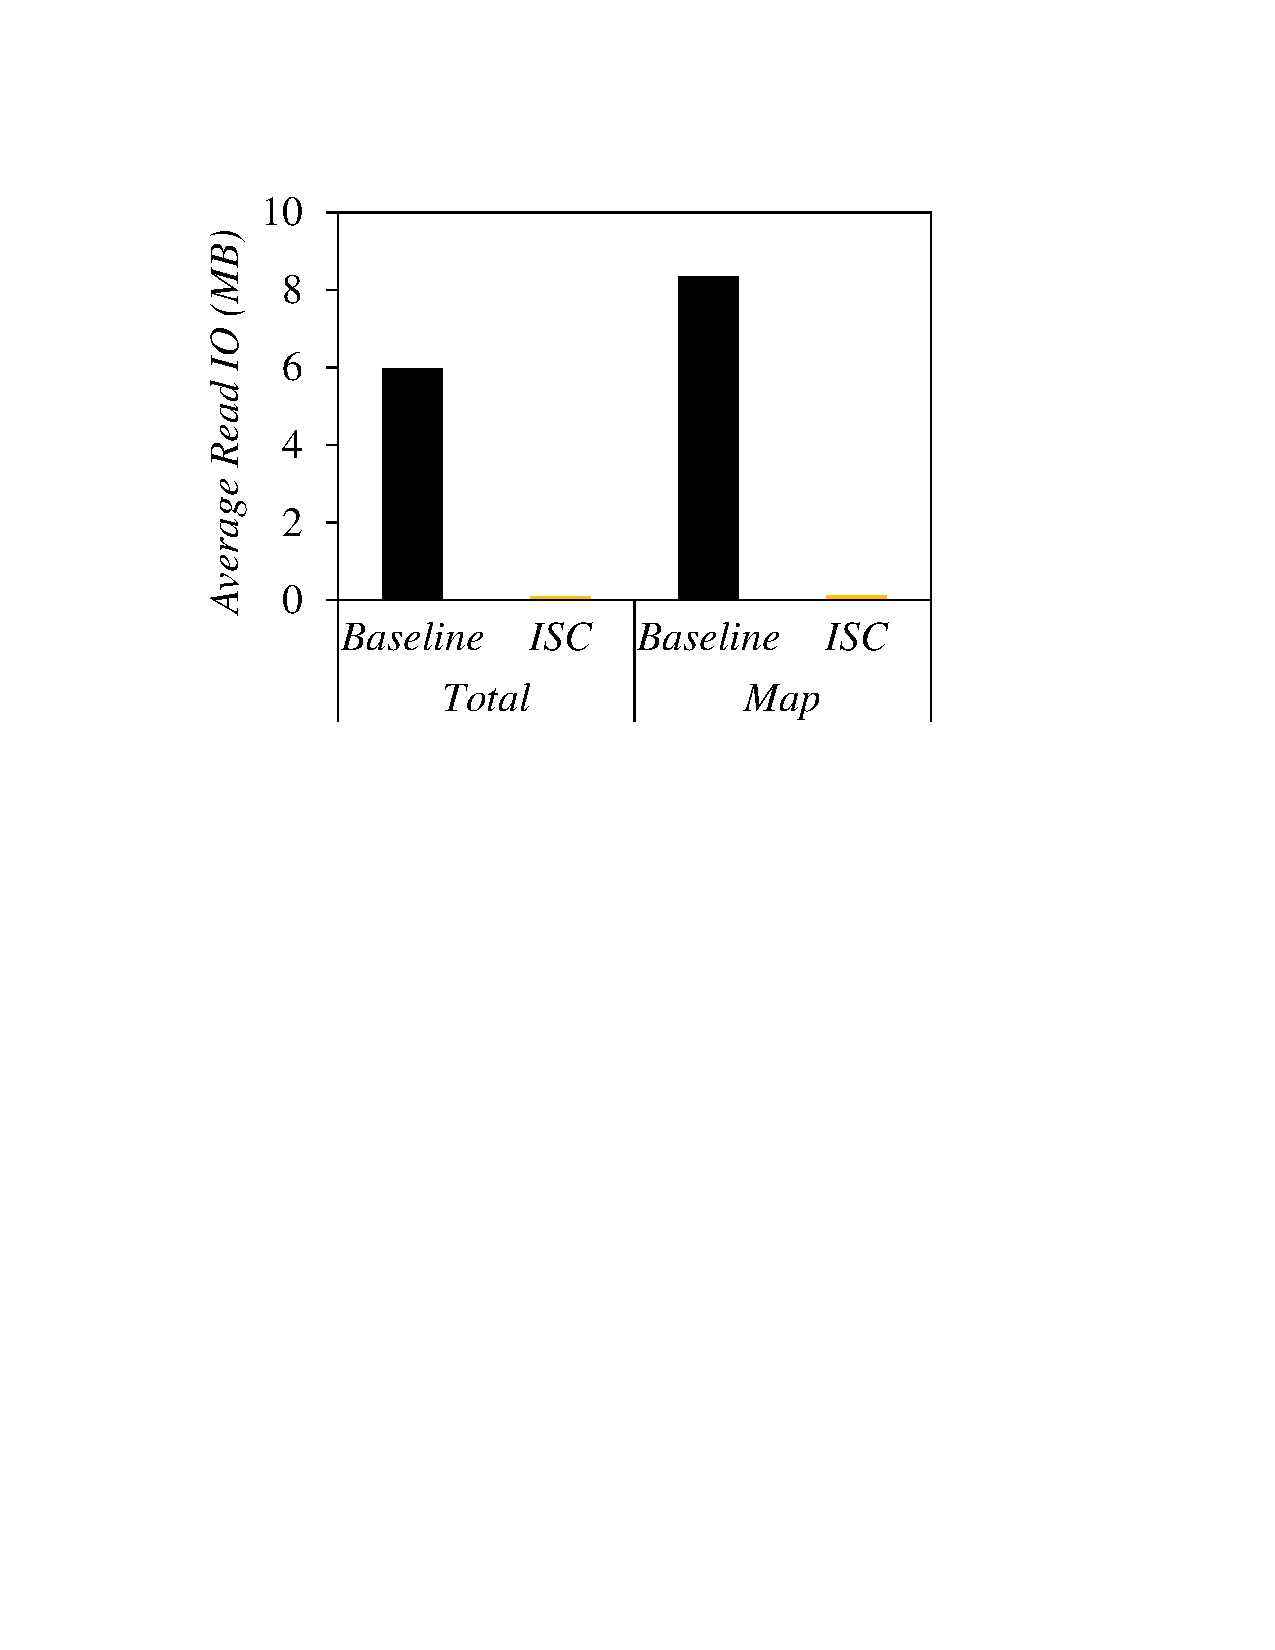
\includegraphics[width=0.66\columnwidth]{figures/Hadoop_average_read_io.pdf}&
  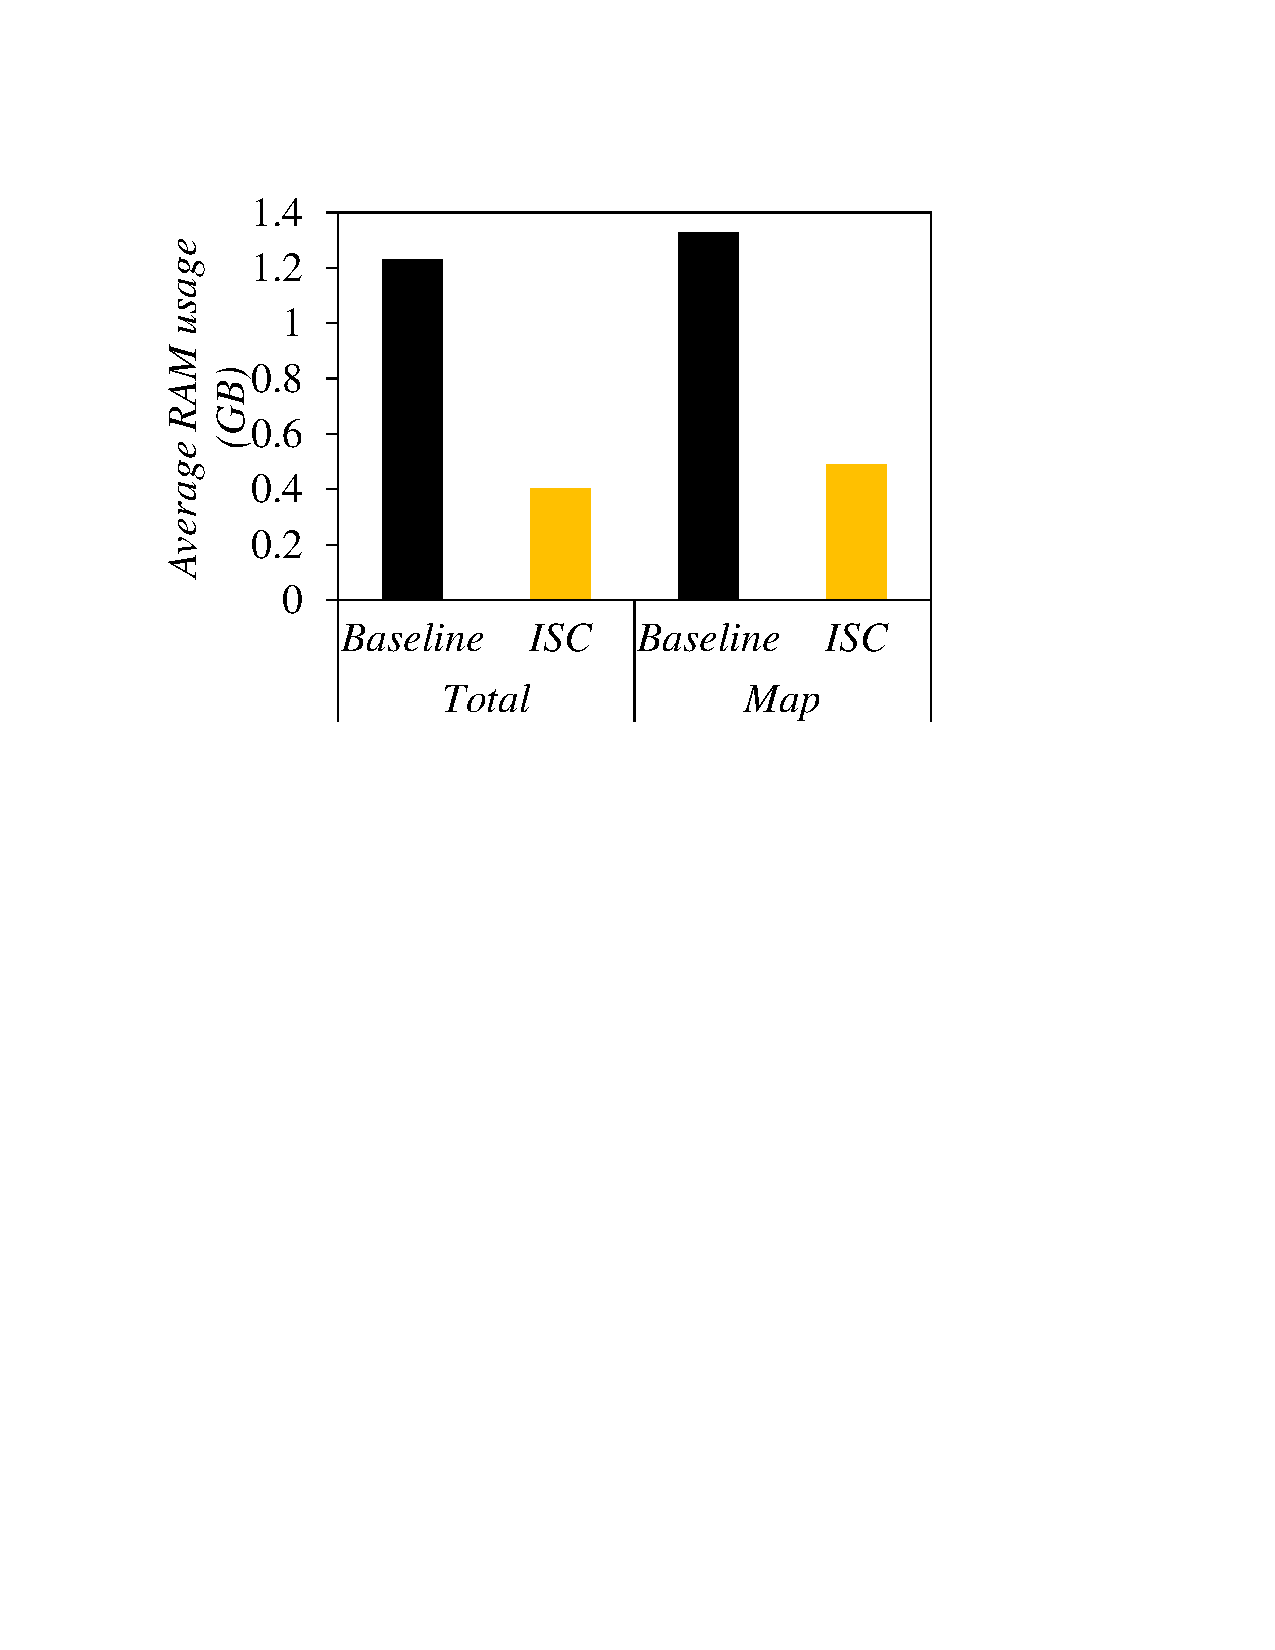
\includegraphics[width=0.66\columnwidth]{figures/Hadoop_average_RAM_usage.pdf}\\	
  (a) Average Host CPU Usage & (b) Average Host Read I/O & (c) Average Host DRAM Usage
\end{tabular}
  \caption{Average host system resource usage}
  \label{fig:avg_host_resource_usage}
\end{figure*}





Now, we add one more ISC device to the host, which configures a single instance of namenode and two instances of datanode in a single node. Figure~\ref{fig:execution_time_with_two_namenode_on_single_node} (a) clearly shows 2$\times$ performance improvement with this configuration. This experiment result provides a meaningful implication that our ISC Hadoop system can offer an equivalent performance of a typical Hadoop system with the lower system cost.






\textbf{Energy consumption:} Figure~\ref{fig:execution_time_with_two_namenode_on_single_node} (b) plots total energy consumption of each Hadoop system. We run the Hadoop application with 10GB data on both systems and measure energy consumption. As stated in subsection~\ref{subsubsec:performance_metrics}, we subtract the idle power (40.5W for the single instance, 45.5W for the two instances configuration) from the total power consumption. Then it is multiplied by the total execution in order to produce the total energy consumption. As shown in Figure~\ref{fig:execution_time_with_two_namenode_on_single_node} (b), our ISC Hadoop system consumes surprisingly lower energy (9$\times$) than the typical Hadoop system with SSDs. Since we measure an additional energy consumption by eliminating an idle system power, both Hadoop systems with single ISC devices (just an SSD for the baseline system) and two ISC devices (two SSDs for the baseline system) show almost the same results. Intuitively, this is because the Hadoop system with two ISC devices (i.e., two instances of datanode) consumes two times more system power but it completes Hadoop job two times faster.
Based on our experimental results, with the help of a faster execution time and lower energy consumption, our ISC Hadoop system can make a notably contribution to reduce a Total Cost of Ownership (TCO). 





\subsubsection{A System Resource Usage}\label{subsubsec:Exp_result_resource_usage}
All key benefits from ISC systems originates from the fact that it does not move data in storage devices to DRAM in the host system. This section clearly verifies this claim. A SATA/SAS bus analyzer is generally adopted to analyze the communication between a host system and devices in a system interface protocol level. This analyzer also provides a graphic user interface to analyze an amount of data transfer between them. As shown in the Figure~\ref{fig:ISC_Hadoop_demo}, we have already demonstrates that ISC Hadoop system does not (or, very rarely) transfer the data from the devices to the host system. 

To make a deeper analysis, we captures three main host system resources: Host CPU usage, Read I/O, and DRAM usage. For this, we set up two Hadoop systems (i.e., ISC and baseline) in a respective single machine with two SSDs (or ISC devices) and run a Hadoop application with 1GB data. We observe each system resource over the execution time (Figure~\ref{fig:host_resource_usage}) and an average resource resource usage respectively (Figure~\ref{fig:avg_host_resource_usage}). 
Moreover, we measure each average value not only during total execution time (refer to Total) but also only Map task execution periods (refer to Map). Interestingly, we observe 8 repetitive ridges in the Figure~\ref{fig:host_resource_usage}. This is because we use 1GB data and configure two datanode instances in a single machine where one Mapper is assigned to each datanode for an accurate analysis. Each datanode executes its own Map task by loading respective input split data of 64MB (that is, 128MB for two Map tasks at the same time). Therefore, we can see 8 separate sections (1GB = 128MB $\times$ 8).

\textbf{Host CPU Usage:} Figure~\ref{fig:host_resource_usage} (a) and Figure~\ref{fig:avg_host_resource_usage} (a) show the host CPU usage during Hadoop application execution time. Both results demonstrate our ISC Hadoop system consumes even less host CPU resources (3.7$\times$ less on total average and 4.2$\times$ less for Map task execution periods). This is because the ISC Hadoop system executes all Map tasks inside the ISC devices thereby using their own CPUs and does not transfer data to the host system for Map task computation. We can observe that intuitively a more CPU resource is consumed for a period of Map task computation.




\begin{figure*}[t]
  \centering
  \renewcommand{\tabcolsep}{2mm}
  \begin{tabular}{ccc}
 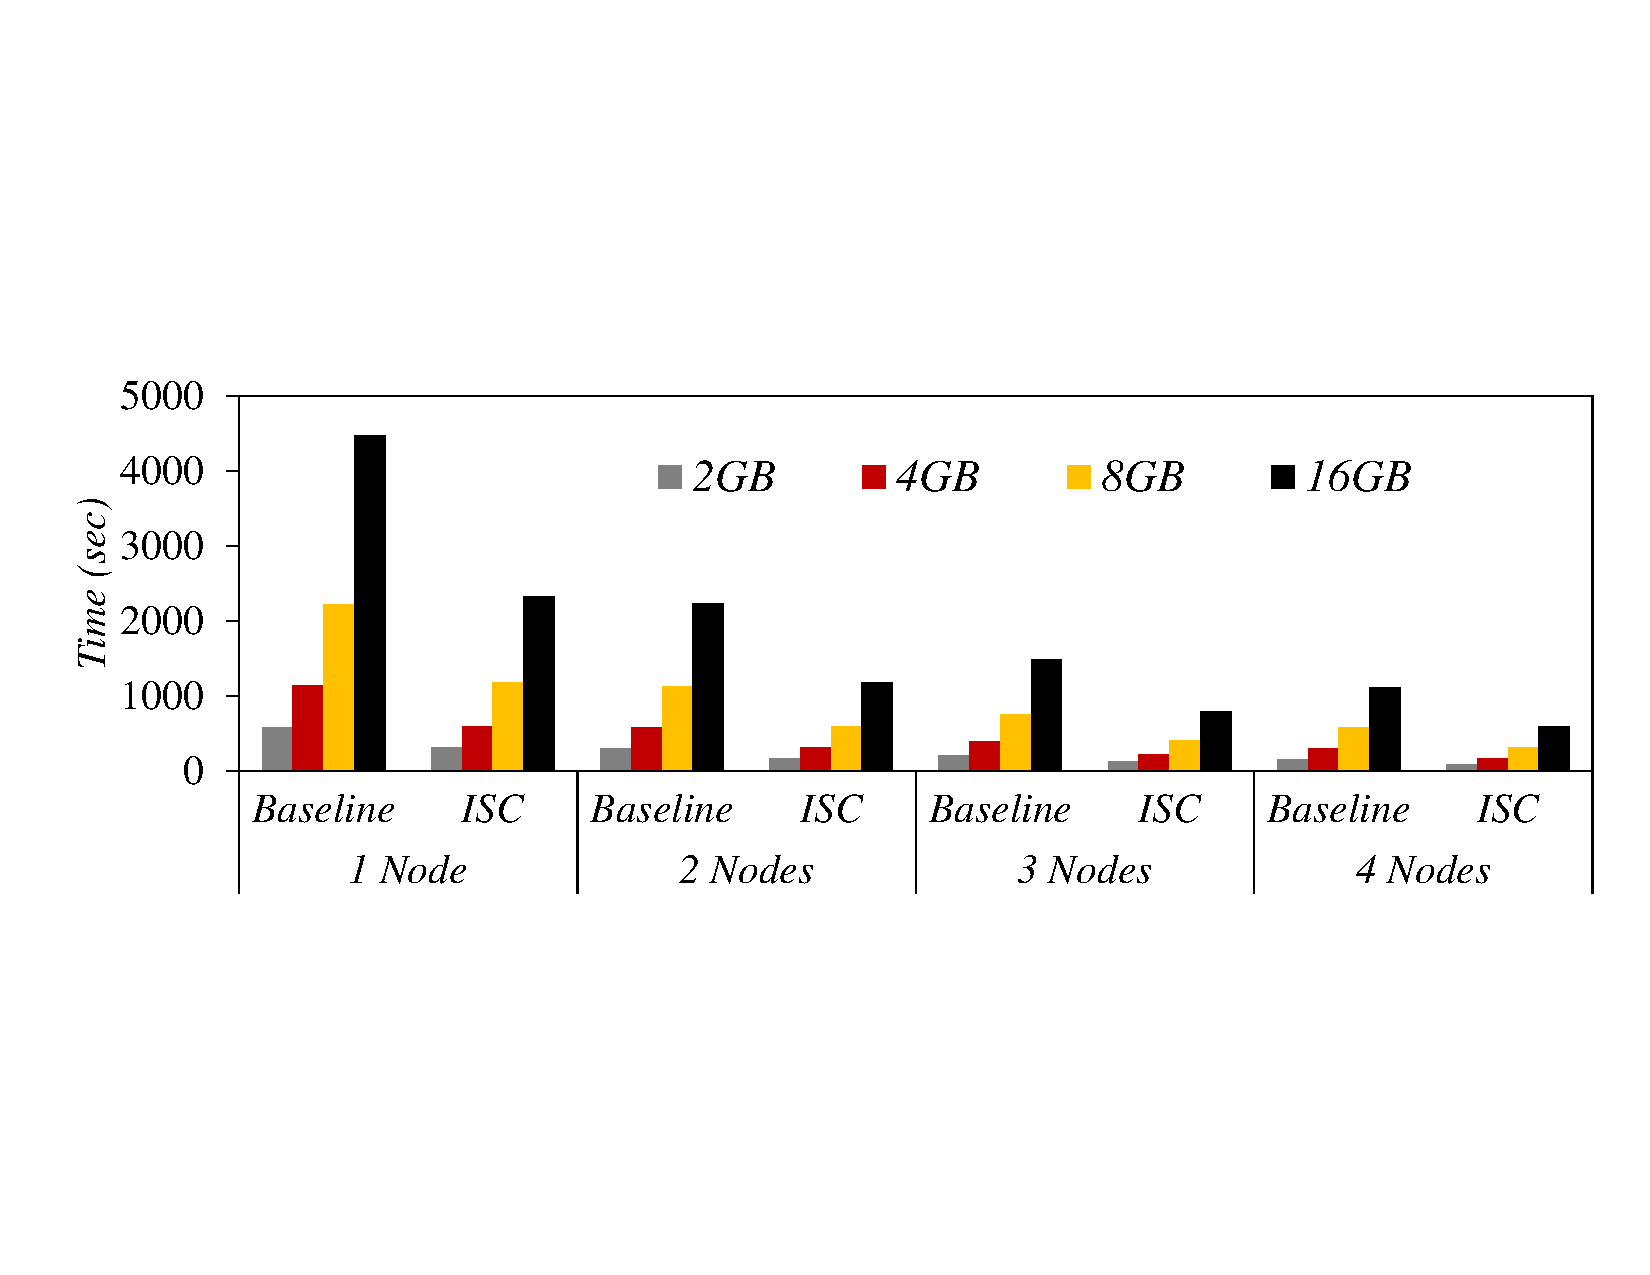
\includegraphics[width=1.25\columnwidth]{figures/Hadoop_total_execution_time_clusters.pdf}&
  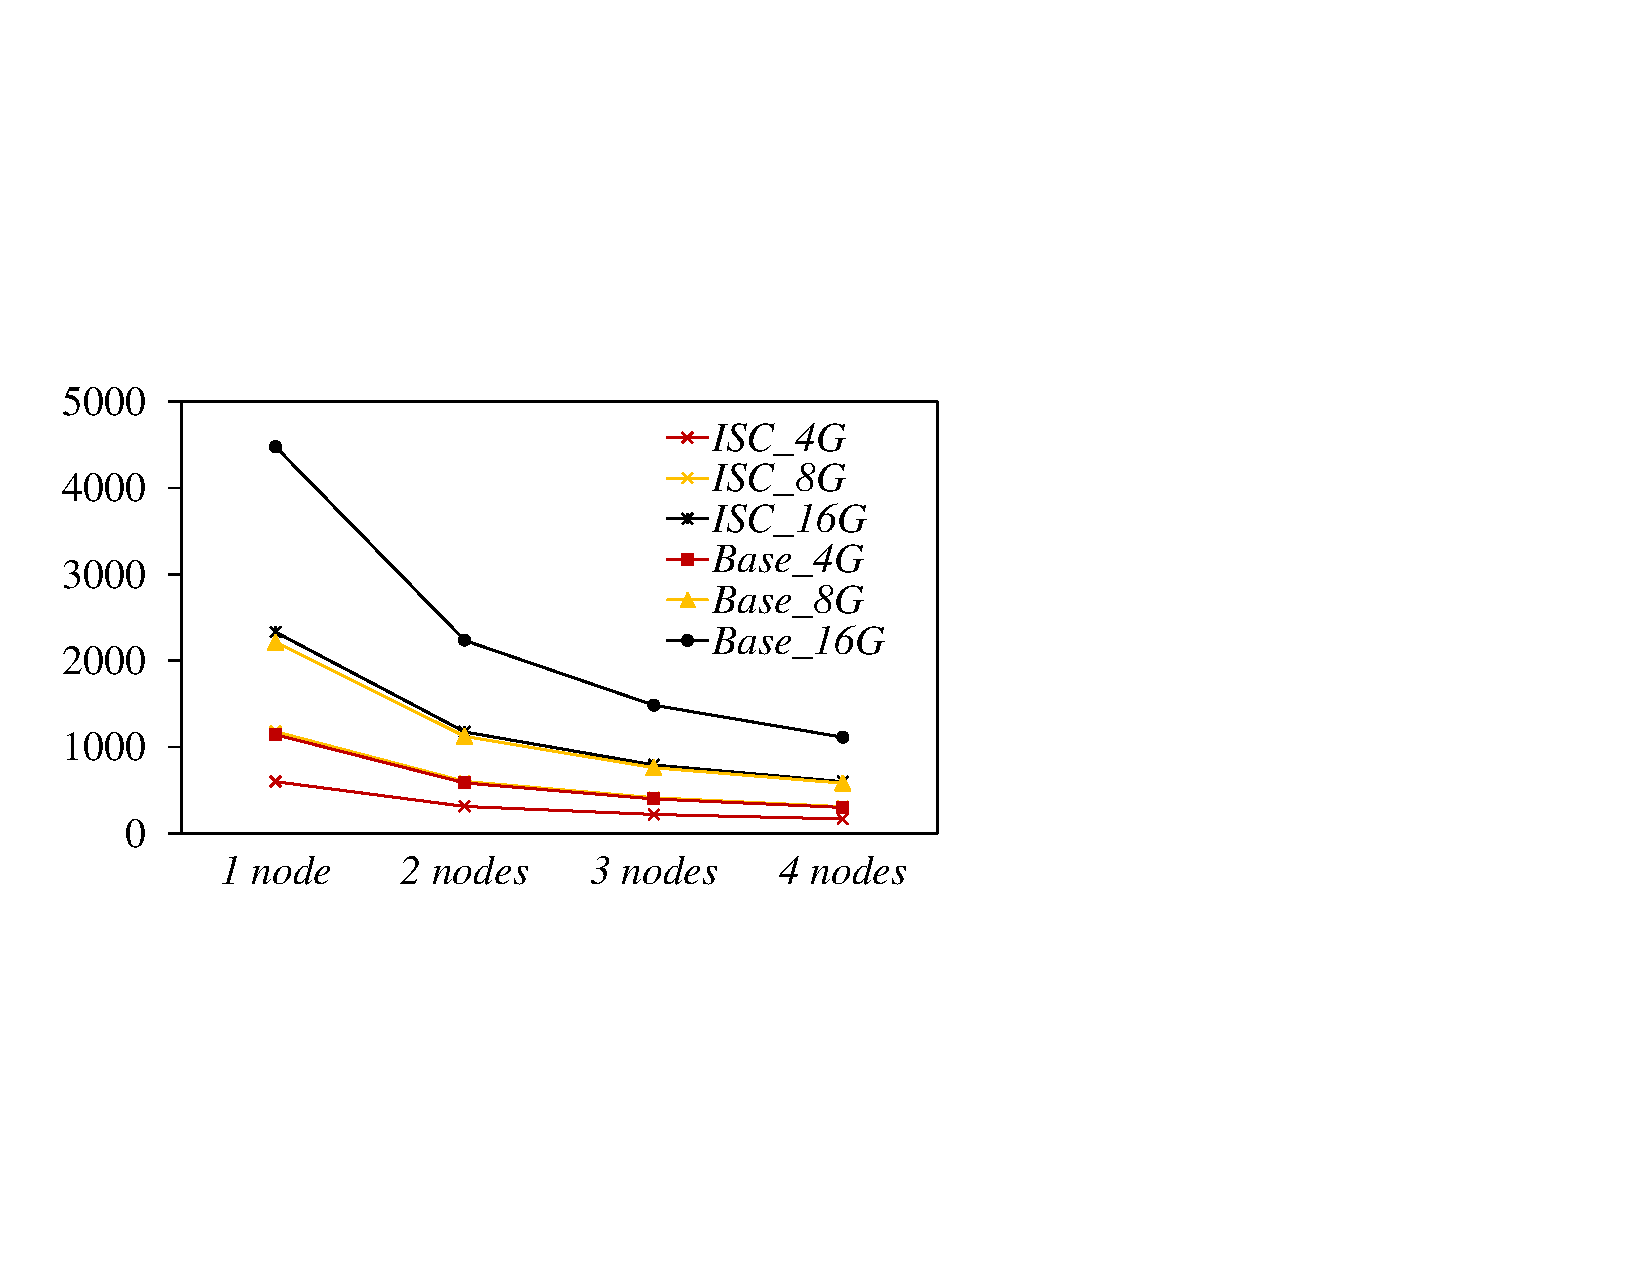
\includegraphics[width=0.75\columnwidth]{figures/Hadoop_total_execution_time_clusters_line.pdf}\\
  (a) Total Elapsed Time & (b) Total Elapsed Time 
\end{tabular}
  \caption{Total elapsed time on Hadoop clusters with a various number of datanode. A node here means datanode.}
  \label{fig:total_time_on_clusters}
\end{figure*}




\begin{figure*}[t]
  \centering
  \renewcommand{\tabcolsep}{2mm}
  \begin{tabular}{ccc}
 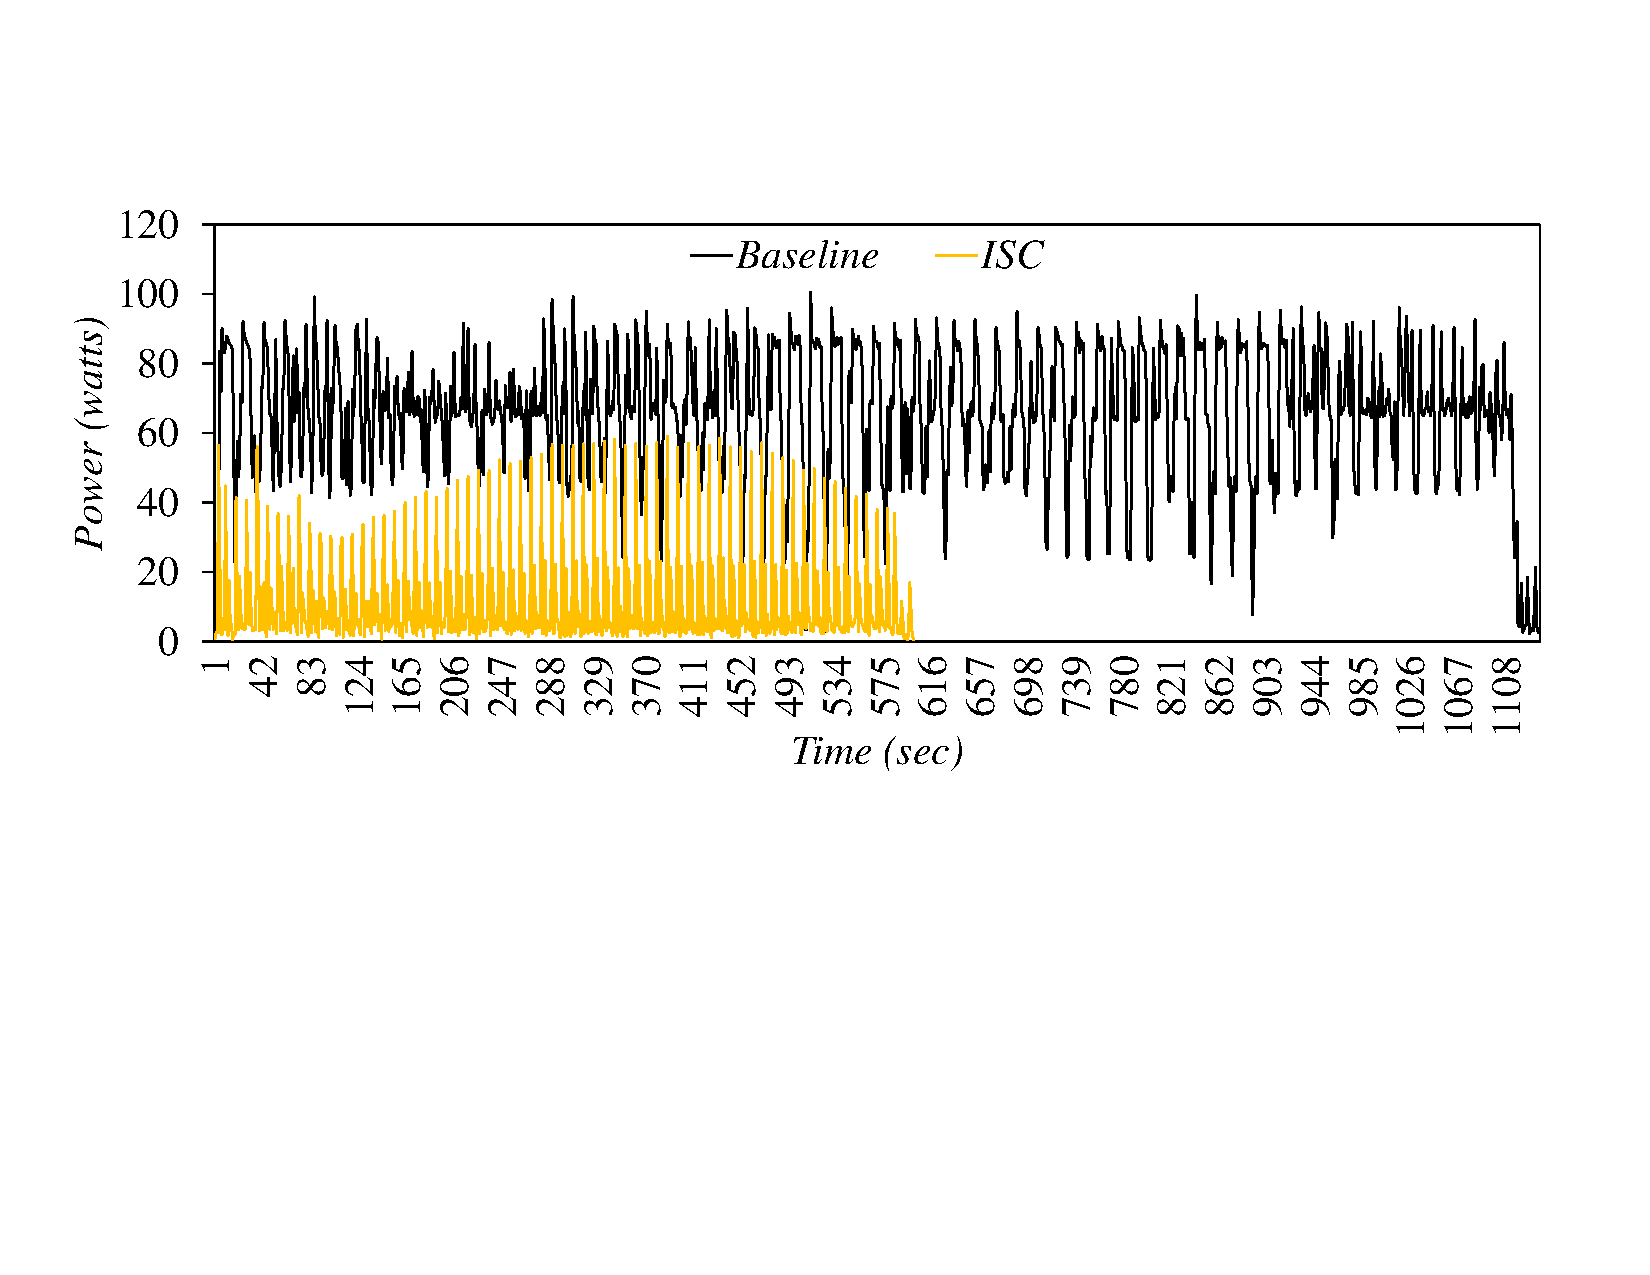
\includegraphics[width=1.25\columnwidth]{figures/Hadoop_power_clusters.pdf}&
  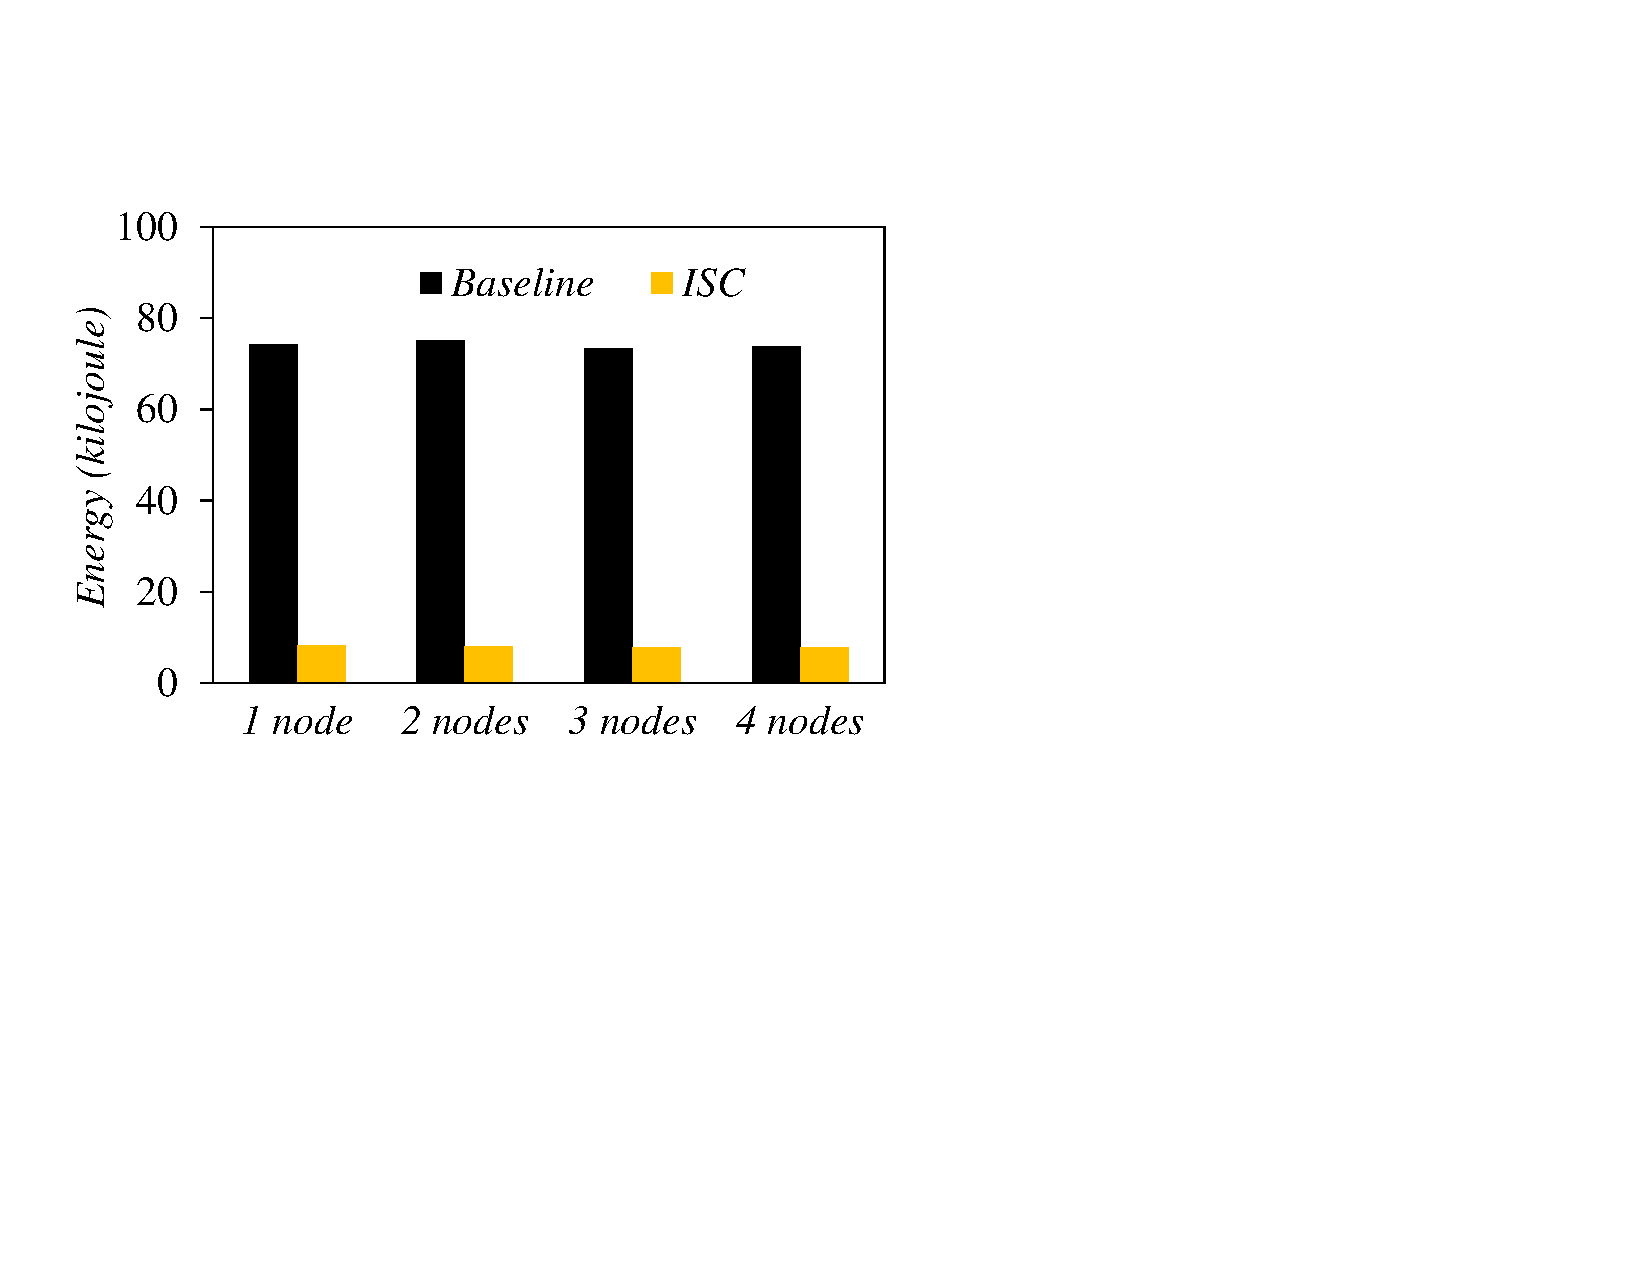
\includegraphics[width=0.75\columnwidth]{figures/Hadoop_energy_clusters.pdf}\\
  (a) Power Consumption Over Time (4 datanodes) & (b) Total Energy Consumption 
\end{tabular}
  \caption{Power and energy consumption on Hadoop clusters with 16GB data}
  \label{fig:total_energy_on_clusters}
\end{figure*}






\textbf{Host Read I/O:} Unlike a conventional CPU-centric system loading all data to the host for computation, an ISC system does not need to move data from a device to the host. This can significantly reduce Host I/O between them. Both Figure~\ref{fig:host_resource_usage} (b) and Figure~\ref{fig:avg_host_resource_usage} (b) support this claim. A typical Hadoop system generates lots of read I/Os to load all data from devices to the host, while our ISC Hadoop system very rarely generates read I/Os (almost 2 orders of magnitude less). Especially for the period of each Map task computation, the typical Hadoop system keeps reading data from the devices. This is also verified by our SATA/SAS bus analyzer (Figure~\ref{fig:ISC_Hadoop_demo}). We capture both read and write I/Os, but write I/Os are almost ignorable (less than 1\%) for this application. Thus, we exhibit only read I/Os in the plots. In addition, we also verified that when we add up all amounts of read I/Os, it is almost equivalent to the input data size of 1GB.






\textbf{Host DRAM Usage:} Host DRAM is another important factor to promote ISC systems. Typically, all data loaded from devices are first stored in host DRAM for computation, which results in a more memory consumption. To measure this host memory consumption, we do not run any other applications after reboot and flush all data/page caches. Thus, both starting points of the plot are almost the same. After running the Hadoop application, the baseline system keeps consuming DRAM until all Map tasks completes. On the other hand, our ISC Hadoop system consumes even less DRAM (3$\times$ less). This has a critical impact on energy consumption since it has been widely known that DRAM takes 25\% -- 40\% of a system power consumption~\cite{DRAM_Power:ISCA:2010,NewServerArch:ISCA:2008,PowerNap:ASPLOS:2009,DisaggregatedMem:ISCA:2009}.







\subsubsection{Hadoop Clusters}\label{subsubsec:Exp_result_clusters}
We set up clusters of 5 nodes (1 namenode and 4 datanodes) to verify whether or not all implications from a single node can be applied to real Hadoop clusters. Each datanode is equipped with a ISC device and connects to each others via 1Gb Ethernet switch. 
We run the same Hadoop application and data varying 1GB to 16GB (we eliminate results with 1GB in the plots). 

Figure~\ref{fig:total_time_on_clusters} (a) shows the total elapsed time on the clusters. The results are very similar to those on a single node: our ISC Hadoop system is 2$\times$ faster than baseline Hadoop system, which implies that ISC Hadoop clusters of a half size can achieve a similar performance to the baseline Hadoop clusters, or that ISC Hadoop clusters of the same size as the baseline Hadoop clusters can process two times amount of data for the same period of time. Figure~\ref{fig:total_time_on_clusters} (b) illustrates well this claim. For instance, the plot of the ISC Hadoop system with 16GB data (ISC\_16G) is almost overlapped with the plot of the baseline Hadoop system with 8GB data (Base\_8G).
We do not display the total Mapper elapsed time since the results are not so much different from the Figure~\ref{fig:total_time_on_clusters}. This is already verified in the Figure~\ref{fig:execution_time_with_single_namenode_on_single_node}.
 
As we analyzed in subsection~\ref{subsubsec:Exp_result_singlenode}, the total energy consumption of each size of clusters is almost identical (about 9.3$\times$ lower) since bigger clusters complete the same task with a shorter time (Figure~\ref{fig:total_energy_on_clusters} (b)). Note: like a sinle node experiment, we also eliminate an idle power. Figure~\ref{fig:total_energy_on_clusters} (a) plots a power consumption over time in the clusters of 4 datanodes (plus 1 namenode) with 16GB data. This shows that the ISC Hadoop system consumes about 4.6$\times$ lower power than the baseline system, which induces over 9$\times$ lower energy consumption considering 2$\times$ faster execution time.









%\begin{table}[tbp]
%\centering\small
%\begin{tabular}{l|l}\hline\hline
%\textbf{Parameters}  &   \textbf{Ranges}   \\\hline
%Number of lists & \textbf{2}, 3, 4, 5, 6, 7, 8\\\hline
%List size skewness factor  & 10000, 1000, \textbf{100}, 10, 1\\\hline
%Intersection ratio  &   0.1\%, \textbf{1\%}, 10\%, 100\%\\\hline
%List size & 1 MB, \textbf{10 MB}, 50 MB, 100 MB\\\hline\hline
%\end{tabular}
%\caption{Parameter setup}\label{tab:synData}
%\end{table}



%\begin{table}[tbp]\small
%\centering
%\begin{tabular}{l|l|l|l|l|l}\hline\hline
%$f$ & $n_1$ & $n_2$ & $n_p$ & estimated ANMP & real ANMP \\\hline
%$1$ & $327680$ & $327680$ & $2564$ & $\frac{n_1+n_2}{n_p}=256$ & $383$ \\\hline
%$10$ & $32768$ & $327680$ & $1408$ & $\frac{n_1\cdot\log n_2}{n_p}=427$ & $640$ \\\hline
%$100$ & $3277$ & $327680$ & $1284$ & $\frac{n_1\cdot\log n_2}{n_p}=47$ & $68$ \\\hline
%$1000$ & $328$ & $327680$ & $1280$ & $\frac{n_1\cdot\log n_2}{n_p}=5$ & $6$ \\\hline\hline
%\end{tabular}
%\caption{The average number of memory accesses per page (ANMP) in Figure~\ref{fig:varyListSkewIntersection}, where $f$ means the skewness factor, $n_1$ and $n_2$ indicate the number of entries in list $A$ and $B$, $n_p$ is the total number of pages. Note that each page is 8 KB and each entry takes 32 bytes. Thus, each page can contain 256 entries.}\label{tab:varyListSkewIntersection}
%\end{table}





%  \begin{figure}[tbp]
%  \centering
%    \begin{tabular}{ccc}
% 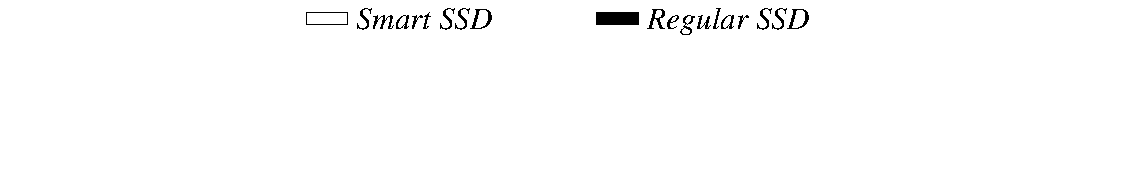
\includegraphics[width=0.52\columnwidth]{figures/banner2.pdf}
%\end{tabular}
%\vspace{-0.1cm}
%\renewcommand{\tabcolsep}{0.1mm}
%  \begin{tabular}{ccc}
% 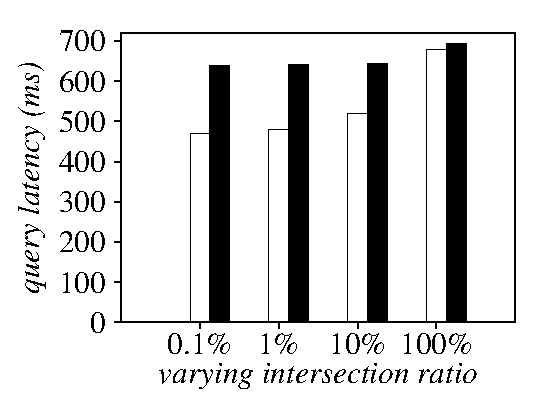
\includegraphics[width=0.5\columnwidth]{figures/Intersection-time-VaryInterRatio-equal2.eps}&
%  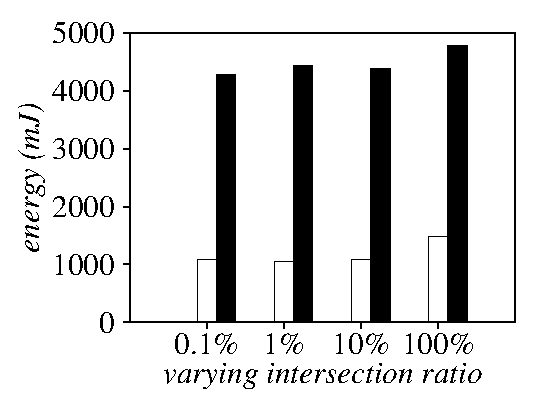
\includegraphics[width=0.5\columnwidth]{figures/Intersection-energy-VaryInterRatio-equal2.eps}\\
%  (a) query latency & (b) energy\\
%\end{tabular}
%  \caption{Varying intersection ratio on equal-sized lists (for intersection)}
%  \label{fig:varyInterRatioIntersection2}
% \end{figure}



%\subsubsection{Discussion: Call for Algorithmic Optimizations}\label{sec:rankUnionOpt}
%Because of too many memory accesses, it is not cost-effective to offload ranked union to Smart SSD.
%To resolve this limitation, on the one hand, we fundamentally need to improve the innate memory access speed of Smart SSDs through the hardware upgrade. On the other hand, more efficient algorithms could be designed to reduce memory access. Our current implementation (following Lucene) solves the ranking problem only if all the union results are available, then scores every qualified document. However, both union and ranking could be algorithmically combined for early termination~\cite{Broder2003EQE,Fagin2001}. This means we do not need to scan all the union results. We will explore the early pruning techniques in the future work. \textcolor{red}{Can delete if no space}

%Because of too many memory accesses, it is not cost-effective to offload ranked union to Smart SSD. To resolve this limitation, on the one hand, we fundamentally need to improve the innate memory access speed of Smart SSD through its hardware update. On the other hand, more efficient algorithms could be designed to reduce memory access. Our current implementation (following Lucene) solves the ranking problem when all the union results are available, then scores every qualified document. However, union and ranking could be algorithmically combined for early termination~\cite{Broder2003EQE,Fagin2001}. Meaning that, we do not need to scan all the union results. We will explore the early pruning techniques in the future work.


%More importantly, one needs to be careful about the \emph{hidden constant} of algorithms, not only big O notation. E.g., the sort-merge based union algorithm is in linear cost, however, the hidden constant factor slows down the performance significantly.



%\textbf{Algorithmically combined (may be a possible)\cite{topk}.}

%\textbf{A special case of ranked union on \emph{two} lists.} If the number of lists is 2, a better algorithm for Smart SSD can be as follows. (1) Find the intersection results $R$ between $k$ lists $L_1, L_2, \cdots, L_k$. It takes, usually, less than 1 scan of all lists; (2) Scan Scan $R$, and $L_1, L_2, \cdots, L_k$ to find the top ranked results. It takes 1 scan. Thus, in total, around 2 full scans on all the $k$ lists. In this case, Samrt SSD wins.


\section{Related Work}\label{sec:relatedWork}
Some studies claim the main idea of offloading a computation into storage devices originates from CASSM or Data Base Computer (DBC) in 1970s~\cite{CASSM:VLDB:1975,DBC:ISCA:1978}. They adopt process-per-track or process-per-head architecture which associates a processing logic with each read/write head of a hard disk drive. As a matter of fact, both Active Disks and iDisks in 1998 start to explore a modern In-Storage Computing (also called In-Storage Processing or In-situ Processing) design~\cite{ActiveDisks:ASPLOS:1998,Keeton1998} with the help of the advance of HDD technologies (i.e., bandwidth growth and cost dropping). They try to offload key application functions such as query operators inside HDDs to reduce data movement, which corresponds to a current In-Storage Computing model. However, still low computing capabilities of HDDs prevent HDD-based ISC from successful landing to practical systems.







%The main idea of offloading computation to storage devices (i.e., In-Storage Computing) has been around for decades. Many research efforts (both hardware and software sides) have been devoted to making it practical.


%\textbf{Early work on In-Storage Computing.} As early as 1970s, some initial work have been proposed to leverage specialized hardware (e.g., processor-per-track~\cite{Su1975} and processor-per-head~\cite{Kannan1978}) for improving query processing in storage devices (i.e., hard disks at that time). However, none of the systems turned out to be successful due to high design complexity and manufacturing cost.

%\textbf{Early work on In-Storage Computing.} As early as 1970s, some pieces of initial work have been proposed to leverage specialized hardware (e.g., processor-per-track and processor-per-head) for improving query processing in storage devices (i.e., hard disks at that time). For example, CASSM~\cite{Su1975} and RAP~\cite{Ozkarahan1977} followed the processor-per-track architecture to embed a processor per each track. The Ohio State Data Base Computer (DBC)~\cite{Kannan1978} and SURE~\cite{LeilichSZ78} followed the processor-per-head architecture to associate processing logic with each read/write head of a hard disk. However, none of the systems turned out to be successful due to high design complexity and manufacturing cost.

%\textbf{Early work on In-Storage Computing.} As early as 1970s, some pieces of initial work have been proposed to leverage specialized hardware (e.g., processor-per-track and processor-per-head) for improving query processing in storage devices (i.e., hard disks at that time). For example, CASSM~\cite{Su1975} % and RAP~\cite{Ozkarahan1977} 
%followed the processor-per-track architecture to embed a processor per each track. 
%The Ohio State Data Base Computer (DBC)~\cite{Kannan1978}  %and SURE~\cite{LeilichSZ78} 
%followed the processor-per-head architecture to associate processing logic with each read/write head of a hard disk. However, none of the systems turned out to be successful due to high design complexity and manufacturing cost.

%\textbf{Later work on HDD In-Storage Computing.}
%In late 1990s, the bandwidth of hard disks (HDD) kept growing while the cost of powerful processors kept dropping, which makes it feasible to offload bulk computation to each individual disk. Researchers started to explore in-storage computing in terms of hard disks (e.g., active disk~\cite{Acharya1998ADP} or intelligent disk~\cite{Keeton1998}). Their goal is to offload application-specific query operators inside hard disk in order to save data movement. They examined active disk in database area by offloading several primitive database operators (e.g., selection, group-by, sort). Later on, Erik et al. extended the application to data mining and multimedia area~\cite{Riedel1998ASL} (e.g., frequent sets mining and edge detection). Although interesting, few real systems adopted the proposals due to various reasons including limited hard disk bandwidth, computing power, and performance gains.



However, the advent of SSDs paves the way for people to rethink of In-Storage Computing as a practical and promising computing model even in industries as well as in the academia. Samsung recently promotes Storage Intelligence for In-Storage Computing and Multi-Stream to improve SSD performance and better NAND flash endurance, which is adopted by storage companies like Pure Storage~\cite{StorageIntelligence:Samsung:PureStorage}. IBM applies ISC to their Blue Gene supercomputers to leverage the high internal bandwidth of SSDs~\cite{IBM:BlueGene:2013}. Oracle's Exadata also starts to offload complex database processing into their storage servers~\cite{Exadata:Oracle:2010}. 

SSD-based ISC attracts academia as well. Logothetis et al. propose iMR for in-situ log processing~\cite{iMR:ATC:2011}. It suggests an architecture with a prototype system based on a best-effort distributed stream processor. Kim et al. try to move a scan operator in database to SSDs based on simulation~\cite{OPCL:ADMS:2011} and later Do et al. integrate Microsoft SQL Server with real SSDs thereby offloading database key operators to the SSDs~\cite{SmartSSD:SIGMOD:2013}. Kang et al. propose Hadoop MapReduce framework for ISC~\cite{SmartSSDHadoop:MSST:2013}. This work addresses same topic as ours; however, it supports only one node with just limited functions. On the other hands, our proposed ISC Hadoop MapReduce framework fully follows the exiting MapReduce framework and can operates on distributed Hadoop clusters. Boboila et al. propose Active Flash to apply ISC to data analytics~\cite{ActiveFlash:MSST:2012} and later Tiwari et al. develop more on this Active Flash for extreme scale machine based on OpenSSD platform~\cite{ActivFlash:FAST:2013,Jasmine:OpenSSD}.
Seshadri et al. propose a Willow system~\cite{Willow:OSDI:2014}. This is a user-programmable SSD prototype system allowing programmers to augment and extend the semantics of an SSD with application-specific features.

Our work explore the opportunities and challenges of Hadoop MapReduce framework based on In-Storage Computing model.





\section{Conclusion}\label{sec:conclusion}

Unlike the traditional CPU-centric computing model, SSD-based In-Storage Computing (ISC) is a new computing paradigm that enables SSDs to play a major role in computation, not just in yet-another-faster HDDs. This SSD-based ISC system offloads main features from a host to an SSD to make the best use of SSD potential capabilities such as its high interval bandwidth and computational power with low power CPUs. 

In this paper, we apply the ISC model to the Hadoop MapReduce framework--a de facto standard distributed computing framework for big data processing. After investigation, we offload Mapper from a host Hodoop system to SSDs and integrate the existing Hadoop MapReduce system with our ISC devices. This system co-design gives rise to the following challenging technical issues: (1) discrepancy in data representation and (2)system interfaces between a host system and a ISC device, (3) Hadoop data split, and (4) feature offloading. To address the data representation and system interface issues, we add a software layer between the host Hadoop framework and our ISC devices. This software interface layer is in charge of converting a file name to LBA information and communicating Java codes with C/C++ codes. The data split issue in HDFS input split data of 64MB (default) is another critical issue. To resolve this, we consult a host Hadoop system to receive the split information and store the split part as a separate data file. Then our ISC Hadoop system process the separate file as new input data. Which part should be offloaded to the ISC device is always a big issue for ISC research and implementation because moving all features to SSDs does not necessarily result in a performance improvement.
A fully distributed mode on a single Hadoop machine is yet-another interesting issue for Hadoop MapReduce research work. Although Hadoop does not support this mode, it can provide a very useful and efficient way by simulating the fully distributed Hadoop clusters only in a single machine. All of our initial studies and analyses have been made on this mode and it can be applied to the real multi-node Hadoop clusters.

Our extensive experiments and results demonstrate that our ISC Hadoop system exhibits a siginficant performance improvement (2$\times$ faster) as well as marvelous energy saving (more than 9$\times$ less) than a typical Hadoop system. Moreover, our deep analyses are provided to delve into our performance gains.

As we mentioned, we classify wordcount-like Hadoop applications as ISC-favorable applications and choose Hadoop wordcount for our experiments. We expect all such applications will show very similar results and remain its verification via a system implementation as our future work. In addition, we can also investigate ISC-nonfavorable Hadoop applications in the future.



%  %%%%%%%%%%%%%%%%%%%%%%%%5
%\clearpage
%\pagestyle{empty}
%\input{department}
%\clearpage






%\setstretch{1}
%\bibliography{ws1,ws2,asplos,fpga,full,hot-chips,immd4,microchip,other,BuildingStuff}


%\begin{small}

%\bibliographystyle{ieeetr}
%\begin{spacing}{0.3}
\small
\balance
\bibliography{paper}

\bibliographystyle{abbrv}
%\bibliographystyle{mbt_dj}
%\end{spacing}
%\end{small}

%\clearpage
%\input{bio}
%\clearpage
%\input{budget}
%\clearpage
%\input{facilities}

\end{document}








%\IEEEraisesectionheading{\section{Introduction}\label{sec:introduction}}
% Computer Society journal (but not conference!) papers do something unusual
% with the very first section heading (almost always called "Introduction").
% They place it ABOVE the main text! IEEEtran.cls does not automatically do
% this for you, but you can achieve this effect with the provided
% \IEEEraisesectionheading{} command. Note the need to keep any \label that
% is to refer to the section immediately after \section in the above as
% \IEEEraisesectionheading puts \section within a raised box.




% The very first letter is a 2 line initial drop letter followed
% by the rest of the first word in caps (small caps for compsoc).
% 
% form to use if the first word consists of a single letter:
% \IEEEPARstart{A}{demo} file is ....
% 
% form to use if you need the single drop letter followed by
% normal text (unknown if ever used by IEEE):
% \IEEEPARstart{A}{}demo file is ....
% 
% Some journals put the first two words in caps:
% \IEEEPARstart{T}{his demo} file is ....
% 
% Here we have the typical use of a "T" for an initial drop letter
% and "HIS" in caps to complete the first word.
%\IEEEPARstart{T}{his} demo file is intended to serve as a ``starter file''
%for IEEE Computer Society journal papers produced under \LaTeX\ using
%IEEEtran.cls version 1.8a and later.
% You must have at least 2 lines in the paragraph with the drop letter
% (should never be an issue)
%I wish you the best of success.

%\hfill mds
 
%\hfill September 17, 2014

%\subsection{Subsection Heading Here}
%Subsection text here.

% needed in second column of first page if using \IEEEpubid
%\IEEEpubidadjcol

%\subsubsection{Subsubsection Heading Here}
%Subsubsection text here.


% An example of a floating figure using the graphicx package.
% Note that \label must occur AFTER (or within) \caption.
% For figures, \caption should occur after the \includegraphics.
% Note that IEEEtran v1.7 and later has special internal code that
% is designed to preserve the operation of \label within \caption
% even when the captionsoff option is in effect. However, because
% of issues like this, it may be the safest practice to put all your
% \label just after \caption rather than within \caption{}.
%
% Reminder: the "draftcls" or "draftclsnofoot", not "draft", class
% option should be used if it is desired that the figures are to be
% displayed while in draft mode.
%
%\begin{figure}[!t]
%\centering
%\includegraphics[width=2.5in]{myfigure}
% where an .eps filename suffix will be assumed under latex, 
% and a .pdf suffix will be assumed for pdflatex; or what has been declared
% via \DeclareGraphicsExtensions.
%\caption{Simulation results for the network.}
%\label{fig_sim}
%\end{figure}

% Note that IEEE typically puts floats only at the top, even when this
% results in a large percentage of a column being occupied by floats.
% However, the Computer Society has been known to put floats at the bottom.


% An example of a double column floating figure using two subfigures.
% (The subfig.sty package must be loaded for this to work.)
% The subfigure \label commands are set within each subfloat command,
% and the \label for the overall figure must come after \caption.
% \hfil is used as a separator to get equal spacing.
% Watch out that the combined width of all the subfigures on a 
% line do not exceed the text width or a line break will occur.
%
%\begin{figure*}[!t]
%\centering
%\subfloat[Case I]{\includegraphics[width=2.5in]{box}%
%\label{fig_first_case}}
%\hfil
%\subfloat[Case II]{\includegraphics[width=2.5in]{box}%
%\label{fig_second_case}}
%\caption{Simulation results for the network.}
%\label{fig_sim}
%\end{figure*}
%
% Note that often IEEE papers with subfigures do not employ subfigure
% captions (using the optional argument to \subfloat[]), but instead will
% reference/describe all of them (a), (b), etc., within the main caption.
% Be aware that for subfig.sty to generate the (a), (b), etc., subfigure
% labels, the optional argument to \subfloat must be present. If a
% subcaption is not desired, just leave its contents blank,
% e.g., \subfloat[].


% An example of a floating table. Note that, for IEEE style tables, the
% \caption command should come BEFORE the table and, given that table
% captions serve much like titles, are usually capitalized except for words
% such as a, an, and, as, at, but, by, for, in, nor, of, on, or, the, to
% and up, which are usually not capitalized unless they are the first or
% last word of the caption. Table text will default to \footnotesize as
% IEEE normally uses this smaller font for tables.
% The \label must come after \caption as always.
%
%\begin{table}[!t]
%% increase table row spacing, adjust to taste
%\renewcommand{\arraystretch}{1.3}
% if using array.sty, it might be a good idea to tweak the value of
% \extrarowheight as needed to properly center the text within the cells
%\caption{An Example of a Table}
%\label{table_example}
%\centering
%% Some packages, such as MDW tools, offer better commands for making tables
%% than the plain LaTeX2e tabular which is used here.
%\begin{tabular}{|c||c|}
%\hline
%One & Two\\
%\hline
%Three & Four\\
%\hline
%\end{tabular}
%\end{table}


% Note that the IEEE does not put floats in the very first column
% - or typically anywhere on the first page for that matter. Also,
% in-text middle ("here") positioning is typically not used, but it
% is allowed and encouraged for Computer Society conferences (but
% not Computer Society journals). Most IEEE journals/conferences use
% top floats exclusively. 
% Note that, LaTeX2e, unlike IEEE journals/conferences, places
% footnotes above bottom floats. This can be corrected via the
% \fnbelowfloat command of the stfloats package.




%\section{Conclusion}
%The conclusion goes here.





% if have a single appendix:
%\appendix[Proof of the Zonklar Equations]
% or
%\appendix  % for no appendix heading
% do not use \section anymore after \appendix, only \section*
% is possibly needed

% use appendices with more than one appendix
% then use \section to start each appendix
% you must declare a \section before using any
% \subsection or using \label (\appendices by itself
% starts a section numbered zero.)
%


%\appendices
%\section{Proof of the First Zonklar Equation}
%Appendix one text goes here.

% you can choose not to have a title for an appendix
% if you want by leaving the argument blank
%\section{}
%Appendix two text goes here.


% use section* for acknowledgment
%\ifCLASSOPTIONcompsoc
  % The Computer Society usually uses the plural form
%  \section*{Acknowledgments}
%\else
  % regular IEEE prefers the singular form
%  \section*{Acknowledgment}
%\fi


%The authors would like to thank...


% Can use something like this to put references on a page
% by themselves when using endfloat and the captionsoff option.
\ifCLASSOPTIONcaptionsoff
  \newpage
\fi



% trigger a \newpage just before the given reference
% number - used to balance the columns on the last page
% adjust value as needed - may need to be readjusted if
% the document is modified later
%\IEEEtriggeratref{8}
% The "triggered" command can be changed if desired:
%\IEEEtriggercmd{\enlargethispage{-5in}}

% references section

% can use a bibliography generated by BibTeX as a .bbl file
% BibTeX documentation can be easily obtained at:
% http://www.ctan.org/tex-archive/biblio/bibtex/contrib/doc/
% The IEEEtran BibTeX style support page is at:
% http://www.michaelshell.org/tex/ieeetran/bibtex/
%\bibliographystyle{IEEEtran}
% argument is your BibTeX string definitions and bibliography database(s)
%\bibliography{IEEEabrv,../bib/paper}
%
% <OR> manually copy in the resultant .bbl file
% set second argument of \begin to the number of references
% (used to reserve space for the reference number labels box)
%\begin{thebibliography}{1}

%\bibitem{IEEEhowto:kopka}
%H.~Kopka and P.~W. Daly, \emph{A Guide to \LaTeX}, 3rd~ed.\hskip 1em plus
%  0.5em minus 0.4em\relax Harlow, England: Addison-Wesley, 1999.

%\end{thebibliography}



\bibliographystyle{IEEETran}
\bibliography{paper}




% biography section
% 
% If you have an EPS/PDF photo (graphicx package needed) extra braces are
% needed around the contents of the optional argument to biography to prevent
% the LaTeX parser from getting confused when it sees the complicated
% \includegraphics command within an optional argument. (You could create
% your own custom macro containing the \includegraphics command to make things
% simpler here.)
%\begin{IEEEbiography}[{\includegraphics[width=1in,height=1.25in,clip,keepaspectratio]{mshell}}]{Michael Shell}
% or if you just want to reserve a space for a photo:

%\begin{IEEEbiography}{Michael Shell}
%Biography text here.
%\end{IEEEbiography}

% if you will not have a photo at all:
%\begin{IEEEbiographynophoto}{John Doe}
%Biography text here.
%\end{IEEEbiographynophoto}

% insert where needed to balance the two columns on the last page with
% biographies
%\newpage

%\begin{IEEEbiographynophoto}{Jane Doe}
%Biography text here.
%\end{IEEEbiographynophoto}

% You can push biographies down or up by placing
% a \vfill before or after them. The appropriate
% use of \vfill depends on what kind of text is
% on the last page and whether or not the columns
% are being equalized.



\begin{IEEEbiography}[{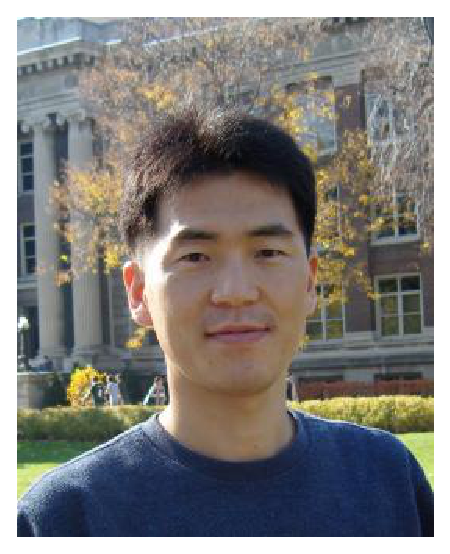
\includegraphics[width=1in,height=1.25in,clip]{figures/dongchul1.eps}}]{Dongchul Park}
is currently a research scientist in System Architecture Lab. (SAL) at Samsung R\&D Center in San Jose, California.  He received his Ph.D. and M.S. degrees in Computer Science and Engineering at the University of Minnesota, Twin Cities in 2012 and 2006 respectively. His research interests lie in storage system design and applications including in-storage computing, big data processing, Hadoop MapReduce, data deduplication, key-value store, non-volatile memories (Flash-based SSDs), hot/cold data identification, embedded systems, and shingled magnetic recording disks.



%is currently a research scientist in System Architecture Lab. (SAL) at Samsung R\&D Center in San Jose, California.  He received his Ph.D. and M.S. degrees in Computer Science and Engineering at the University of Minnesota, Twin Cities in 2012 and 2006 respectively. During his Ph.D., he was a member of Center for Research in Intelligent Storage (CRIS) group and advised by Professor David. H.C. Du. His research interests lie in storage system design and applications including non-volatile memories (Flash-based SSD), hot/cold data identification, embedded systems, shingled magnetic recording disks, data deduplication, home storage systems, and big data/Hadoop.


%is a currently Ph.D. candidate in Computer Science and Engineering at the University of Minnesota, Twin Cities. He received his M.S. degree in Computer Science and Engineering at the University of Minnesota, Twin Cities and at Seoul National University, Korea, in 2006 and 2003 respectively. His research interests include Solid State Drive(SSD) design and its applications, non-volatile memory, Shingled Write Disks, and file/storage systems including data deduplication and home storage systems.





%is a currently Ph.D. candidate in Computer Science and Engineering at the University of Minnesota, Twin Cities. He received his M.S. degree in Computer Science and Engineering at the University of Minnesota, Twin Cities and at Seoul National University, Korea, in 2006 and 2003 respectively. His research interests include Solid State Drive(SSD) design and its applications, non-volatile memory, and file/storage systems including home storage systems.

\end{IEEEbiography}

\vspace{-15mm}

% if you will not have a photo at all:
%\begin{IEEEbiographynophoto}{Biplob Debnath}
%\begin{IEEEbiography}[{\includegraphics[width=1in,height=1.25in,clip,keepaspectratio]{biplob.eps}}]{Biplob Debnath}
\begin{IEEEbiography}[{\includegraphics[width=1in,height=1.25in,clip]{figures/biplob.eps}}]{Kwanghyun Park}
is a research staff member at NEC Laboratories America, Princeton, New Jersey. He received the Ph.D. degree in Electrical and Computer Engineering from the University of Minnesota, Twin Cities in 2010, and the and B.S. degree in Computer Science and Engineering from Bangladesh University of Engineering and Technology, Bangladesh, in 2002. His research interests include Non-volatile memory, data deduplication, key-value store, and storage systems.
\end{IEEEbiography}
%\end{IEEEbiographynophoto}

% insert where needed to balance the two columns on the last page with
% biographies
%\newpage

\vspace{-15mm}

%\begin{IEEEbiographynophoto}{David H.C. Du}
%\begin{IEEEbiography}[{\includegraphics[width=1in,height=1.25in,clip,keepaspectratio]{du2.eps}}]{David H.C. Du}
\begin{IEEEbiography}[{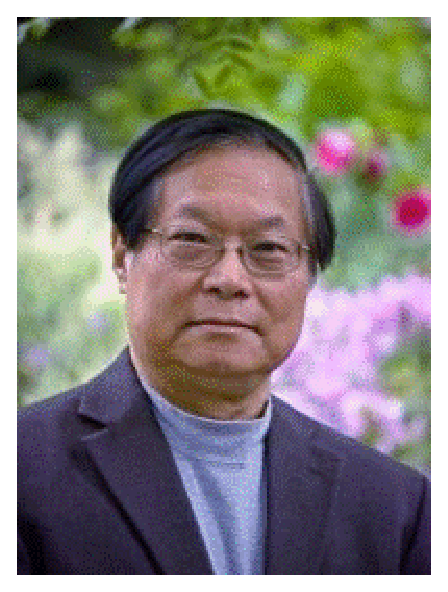
\includegraphics[width=1in,height=1.25in,clip]{figures/du.eps}}]{Yang-Suk Kee}
(Fellow, IEEE) is currently the Qwest Chair Professor in Computer Science and Engineering Department, University of Minnesota, Twin Cities. He received the B.S. degree in mathematics from National Tsing-Hua University, Taiwan, R.O.C. in 1974, and the M.S. and Ph.D.
degrees in computer science from the University of Washington, Seattle, in 1980 and 1981, respectively.  His research interests include storage systems, cyber security, sensor networks, multimedia computing, and high-speed networking.
\end{IEEEbiography}





\vspace{-15mm}

%\begin{IEEEbiographynophoto}{David H.C. Du}
%\begin{IEEEbiography}[{\includegraphics[width=1in,height=1.25in,clip,keepaspectratio]{du2.eps}}]{David H.C. Du}
\begin{IEEEbiography}[{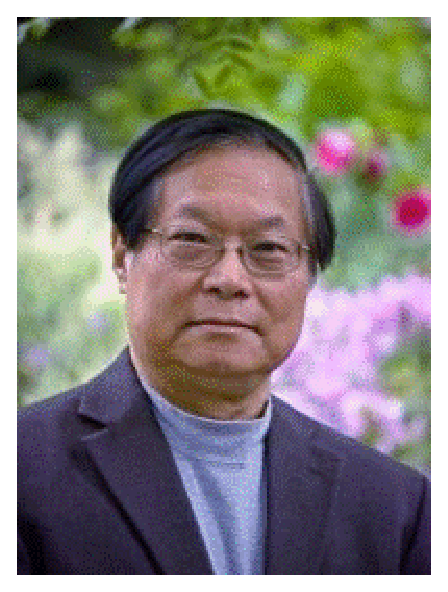
\includegraphics[width=1in,height=1.25in,clip]{figures/du.eps}}]{Jignesh M. Patel}
(Fellow, IEEE) is currently the Qwest Chair Professor in Computer Science and Engineering Department, University of Minnesota, Twin Cities. He received the B.S. degree in mathematics from National Tsing-Hua University, Taiwan, R.O.C. in 1974, and the M.S. and Ph.D.
degrees in computer science from the University of Washington, Seattle, in 1980 and 1981, respectively.  His research interests include storage systems, cyber security, sensor networks, multimedia computing, and high-speed networking.
\end{IEEEbiography}







%\vfill

% Can be used to pull up biographies so that the bottom of the last one
% is flush with the other column.
%\enlargethispage{-5in}



% that's all folks
\end{document}


